\documentclass[12pt,notitlepage]{report}
\usepackage{fullpage}
\usepackage{setspace}\doublespacing
\textfloatsep 0.75in
\usepackage[nottoc]{tocbibind}
\usepackage[super,sort&compress]{natbib}
\usepackage{amsmath}
\usepackage{pgfornament}
\usepackage[bindingoffset=6mm,twoside]{geometry}
\usepackage[toc]{appendix}
\usepackage[english]{babel}
\usepackage{cleveref}
\usepackage[version=3]{mhchem}
\usepackage{pdflscape}
\usepackage{threeparttable}
\usepackage{longtable}
\usepackage{capt-of}
\usepackage{afterpage}
\usepackage{xspace}
\usepackage{subfig}
\usepackage{graphicx}
\usepackage{algorithm}% http://ctan.org/pkg/algorithms
\usepackage{algpseudocode}% http://ctan.org/pkg/algorithmicx
\usepackage{url}

% Control header sizes
\usepackage{titlesec}
\usepackage{lmodern}
\newcommand{\chapfnt}{\fontsize{14}{16}}
\newcommand{\secfnt}{\fontsize{12}{14}}
\newcommand{\ssecfnt}{\fontsize{12}{14}}
\titleformat{\chapter}[display]
{\normalfont\chapfnt\bfseries}{\chaptertitlename\ \thechapter}{20pt}{\chapfnt}
\titleformat{\section}
{\normalfont\secfnt\bfseries}{\thesection}{1em}{}
\titleformat{\subsection}
{\normalfont\ssecfnt\bfseries}{\thesubsection}{1em}{}

% Use symbolic rather than numeric footnotes
\usepackage[symbol]{footmisc}
\renewcommand{\thefootnote}{\fnsymbol{footnote}}

% Reduce vertical spacing in tables and arrays
\renewcommand*{\arraystretch}{0.6}

% Define some macros
\newcommand{\hartree}{\ensuremath{E_\mathrm{h}}\xspace}
\newcommand{\mhartree}{\ensuremath{\mathrm{m}E_\mathrm{h}}\xspace}
\newcommand{\kcal}{\ensuremath{\mathrm{kcal}~\mathrm{mol}^{-1}}\xspace}
\newcommand{\eV}{\ensuremath{\mathrm{eV}}\xspace}
\newcommand{\au}{\ensuremath{\mathrm{a.u.}}\xspace}
\newcommand{\bohr}{\ensuremath{a_0}\xspace}
\newcommand{\std}{\ensuremath{\Delta_\mathrm{SD}}\xspace}
\newcommand{\mae}{\ensuremath{\Delta_\mathrm{MAE}}\xspace}
\newcommand{\rel}{\ensuremath{\Delta_\mathrm{rel}}\xspace}
\newcommand{\termsymbol}[1]{\ensuremath{\mathrm{#1}}\xspace}
\newcommand{\re}{\ensuremath{r_\mathrm{e}}\xspace}

% Title
\newcommand{\dissertationtitle}{%
    Density Cumulant Theory\\for Ground and Excited Electronic states}
\newcommand{\whoami}{Andreas Victor Copan}

\setcounter{tocdepth}{1}

\begin{document}

% Make the official abstract page
\newpage
\thispagestyle{empty}
\vspace*{15pt}
\begin{samepage}
\begin{center}
\textsc{\large{\dissertationtitle}}\\[15pt]
by\\[15pt]
\textsc{\whoami}\\[12pt]
(Under the Direction of Henry F. Schaefer III)\\[12pt]
\textsc{Abstract}
\end{center}
Density cumulant theory (DCT) describes the state of an electronic system by
variationally optimizing a parametrization of the two-particle density cumulant.
The cumulant is a statistical descriptor of the electronic density distribution
which naturally decouples independent subsystems, leading to desirable
properties like size-extensivity which have given the coupled-cluster methods
pride of place in electronic structure theory.
We present benchmarks calculations demonstrating the superior performance of
density cumulant theory relative to coupled-cluster theory for the description
of ground-state properties.
Next, we extend this method for the description of excited states using linear
response theory.
Finally, we develop algorithms for the new excited state model which enable us
to study larger systems such as hexatriene with this new model.
\thispagestyle{empty}
\begin{list}{\textsc{Index words:\hfill}}{\labelwidth 1.2in\leftmargin 1.4in\labelsep 0.2in}
\item 
\begin{flushleft}\singlespacing
    Electronic structure theory, cumulants, density matrices, linear response
    theory, excited states, coupled-cluster theory
\end{flushleft}
\end{list}
\end{samepage}

% Make the official title page
\newpage
\pagenumbering{roman}
\thispagestyle{empty}
\vspace*{18pt}
\begin{center}
\textsc{\large{\dissertationtitle}}\\[18pt]
by\\[18pt]
\textsc{\whoami}\\[12pt]
B.A., Bethel University, 2013\\
\vfill
A Dissertation Submitted to the Graduate Faculty \\
of The University of Georgia in Partial Fulfillment \\
of the \\
Requirements for the Degree \\[10pt]
\textsc{Doctor of Philosophy}\\[36pt]
\textsc{Athens, Georgia}\\[18pt]
2018
\end{center}

% Make the copyright page
\newpage
\thispagestyle{empty}
\vspace*{5.5in}
\begin{center}
\copyright 2018 \\
\whoami \\
All Rights Reserved
\end{center}

% Make the approval page
\newpage
\thispagestyle{empty}
\vspace*{18pt}
\begin{center}
\textsc{\large{\dissertationtitle}}\\[18pt]
by\\[18pt]
\textsc{\whoami}
\end{center}
\vfill
\begin{flushleft}\singlespacing
\hskip 200pt {Approved:}\\
\vspace{12pt}

\hspace*{200pt}\makebox[100pt][l]{Major Professor:}Henry F.~Schaefer III\\
\vspace{12pt}
\hspace*{200pt}\makebox[100pt][l]{Committee:}Gary E.~Douberly\\
\hspace*{200pt}\makebox[100pt][l]{}Henning Meyer\\
% Approval words
\vfill
Electronic Version Approved:\\[12pt]
Suzanne Barbour\\
Dean of the Graduate School\\
The University of Georgia\\
December 2018
\end{flushleft}

\newpage
\vspace*{1.5in}
\begin{center}
\emph{In memory of Valery Andreiyevich and Valtraut Kirsch Copan}\\
\vspace{6pt}
\pgfornament[width=4cm,color=black]{88}
\end{center}

%\chapter*{Acknowledgments}
\addcontentsline{toc}{chapter}{Acknowledgments}

All of your acknowledgments should go here.
\lipsum


\tableofcontents
\clearpage
\pagenumbering{arabic}

% Chapters. Organize and name as you wish, as long as these refer to files that exist.
%%%%%%%%%%%%%%%%
% INTRODUCTION %
%%%%%%%%%%%%%%%%
\chapter{Introduction}

% TODO: Include a second citation. Include \eg \ie examples. Include references. Include em dash.
Here is the introduction. My dissertation introduces \emph{widgets}. If I wish
to cite someone, I could refer to them in text as in \citet{zongker2006chicken},
or parenthetically \citep{zongker2006chicken}. I can also cite just the
year \citeyearpar{zongker2006chicken} or mention the author,
\citeauthor{zongker2006chicken}.


\begin{quote}
This dissertation template is handy. I like it and use it every time I write a
dissertation.\\
\hspace*{\fill} --- Abraham Lincoln \citeyearpar{zongker2006chicken}
\end{quote}


\section{Stuff}
\label{sec:stuff}

Here is a section on stuff.

\subsection{Artificial Neural Networks}
\label{sec:neuralnet}

See Figure~\ref{fig:neuralnet} for a neural network.

\begin{figure}[th]
	\begin{center}
	   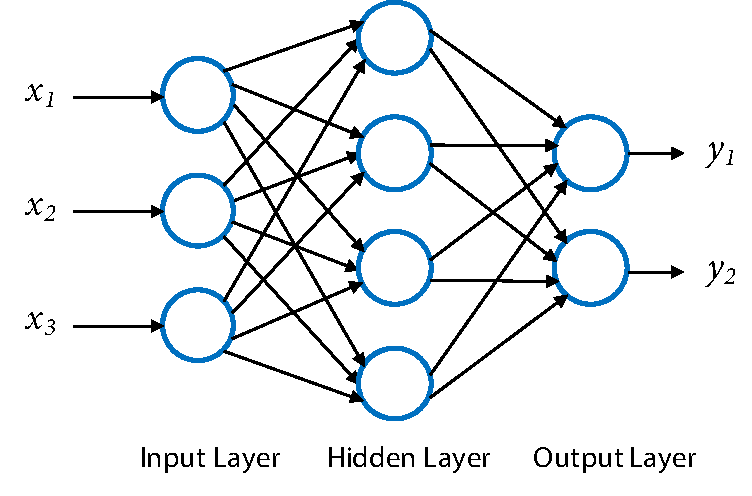
\includegraphics[width=0.8\linewidth]{figures/neuralnet}
	\end{center}
	\caption[An example neural network with two final outputs]
		{An example neural network with two final outputs. Notice how each
		neuron in one layer connects to each neuron in the following layer. This
		is called \emph{fully connected}.}
	\label{fig:neuralnet}
\end{figure}

Cool.

\chapter[%
	Ground-State Density Cumulant Theory:\\
	Thermochemical and Kinetic Benchmark Calculations
]{%
	Ground-State Density Cumulant Theory:\\
	Thermochemical and Kinetic Benchmark Calculations\footnote{%
        A.~V.~Copan, A.~Yu.~Sokolov, and H.~F.~Schaefer.,
        J.~Chem.~Theory~Comput.
        {\bfseries 10},
        2389
        (2014).
        Adapted with permission of the American Chemical Society.
    }
}
\label{ch:benchmark}

\section{Abstract}
We present an extensive benchmark study of density cumulant functional theory
(DCFT) for thermochemistry and kinetics of closed- and open-shell molecules. The
performance of DCFT methods (DC-06, DC-12, ODC-06, and ODC-12) is compared to
that of coupled-electron pair methods (CEPA$_0$ and OCEPA$_0$) and
coupled-cluster theory (CCSD and CCSD(T)) for the description of noncovalent
interactions (A24 database), barrier heights of hydrogen-transfer reactions
(HTBH38), radical stabilization energies (RSE30), adiabatic ionization energies
(AIE), and covalent bond stretching in diatomic molecules. Our results indicate
that out of four DCFT methods the ODC-12 method is the most reliable and
accurate DCFT formulation to date. Compared to CCSD, ODC-12 shows superior
results for all benchmark tests employed in our study. With respect to
coupled-pair theories, ODC-12 outperforms CEPA$_0$, and shows similar accuracy
to the orbital-optimized CEPA$_0$ variant (OCEPA$_0$) for systems at equilibrium
geometries. For covalent bond stretching, ODC-12 is found to be more reliable
than OCEPA$_0$. For the RSE30 and AIE datasets, ODC-12 shows competitive
performance with CCSD(T). In addition to benchmark results, we report new
reference values for the RSE30 dataset computed using coupled cluster theory
with up to perturbative quadruple excitations.


\section{Introduction}

Recent developments in {\itshape ab initio} quantum chemistry have resulted in a
variety of computational models for studying molecules.
Apart from concerns about efficiency and accuracy, several concepts have evolved
as criteria for judging the merits of a particular method.
Energy-based criteria typically define an ``ideal'' approximation as one
yielding correlation energies that are size-consistent,
extensive\cite{Nooijen:2005p2277},
well-defined (giving continuous, unique potential surfaces), and
variational.\cite{Pople:1976p1} 
While it has been argued that the practical benefits of variationality are
rather limited,\cite{Bartlett:1981p359} 
the efficiency of gradient computations, at least, is improved by formulating a
theory in terms of a Hermitian and stationary energy
functional.\cite{Szalay:1995p281}
With respect to scope and stability, methods that show consistent performance
for open-shell systems, strongly correlated states, and non-equilibrium
geometries are particularly valuable.\cite{Bartlett:1981p359}

The incorrect scaling of truncated configuration interaction (CI) energies with
system size has inspired the development of size-extensive alternatives. Among
the earliest formulations, the coupled electron pair approximations (CEPAs)
\cite{Kelly:1963p2091,Kelly:1964pA1450,Meyer:1973p1017,Ahlrichs:1979p31,Koch:1981p387}
attracted much attention in
1970s,\cite{Gelus:1970p503,Staemmler:1972p187,Ahlrichs:1975p1235,Kollmar:1977p3583,Wasilewski:1988p1289}
offering rigorous extensivity and size-consistency while retaining much of the
linearity\cite{Taube:2009p1441122} of CI in their equations.
CEPA methods, however, have been shown to rapidly deteriorate as the molecular
geometry deviates from equilibrium\cite{Taube:2009p1441122} and yield energies
that vary under the rotation of the occupied orbitals.\cite{Ahlrichs:1979p31}
Partly in light of such defects, CEPA has been largely displaced by
coupled-cluster (CC)
theory.\cite{Coester:1958p421,Coester:1960p477,Cizek:1966p4256,Bartlett:1978p561,Bartlett:1981p359,Crawford:2000p33,Bartlett:2007p291,Shavitt:2009}
In addition to size-extensivity, CC offers orbital invariance and improved
stability for non-equilibrium structures\cite{Taube:2009p1441122}, but has a
non-Hermitian energy functional and non-linear equations which are not readily
amenable to parallel implementation.
Although neither class of methods is strictly variational, VCEPA (variational
CEPA) has been shown to be effectively equivalent to its non-variational
counterpart.\cite{Kollmar:2010p2449}
Various other modifications to resolve the deficiencies of traditional CEPA have
been explored, including self-consistent size-consistent CI,
\cite{Daudey:1993p1240,Malrieu:2010p179} orbital-invariant CEPA,
\cite{Nooijen:2006p25,Kollmar:2011p084102} and orbital-optimized CEPA
formulations.
\cite{Kollmar:2010p311,Bozkaya:2013p054104,Soydas:2014p1073,Bozkaya:2013p154105}
Recently, the CEPA methods have been revived by Neese and
co-workers\cite{Wennmohs:2008p217,Neese:2009p114108,Kollmar:2010p2449} who
developed the local pair-natural-orbital CEPA (LPNO-CEPA) methods and have
implemented them for massively parallel computer architectures.

It has recently been
demonstrated\cite{Kutzelnigg:2006p171101,Mazziotti:2008p253002,Mazziotti:2010p062515,DePrince:2012p1917}
that CEPA methods naturally arise in the context of theories that obtain the
molecular energies from density cumulants, the connected and extensive
components of the reduced density matrices
(RDMs).\cite{Kutzelnigg:1997p432,Mazziotti:1998p419,Mazziotti:1998p4219,Kutzelnigg:1999p2800,Kong:2011p3541,Hanauer:2012p50}
The advantage of cumulant-based theories is that, unlike their RDM-based
counterparts,\cite{Nakata:2009p042109,vanAggelen:2010p114112,Verstichel:2010p114113}
they are naturally size-extensive and
size-consistent.\cite{Kutzelnigg:1999p2800,Herbert:2007p261}
We have recently achieved the first
implementation\cite{Simmonett:2010p174122,Sokolov:2012p054105} of density
cumulant functional theory (DCFT), proposed by Kutzelnigg in
2006.\cite{Kutzelnigg:2006p171101}
In DCFT, the molecular energy is obtained in terms of a mean-field one-particle
RDM and the two-particle density cumulant, constrained to be at least
approximately $N$-representable ({\it i.e.}\@ to correspond to a physical
$N$-electron wavefunction).
Like traditional CC theory, DCFT is size-extensive and orbital-invariant, but it
has the additional advantage of a stationary and Hermitian energy functional,
which simplifies the computation of molecular properties.
In the original DCFT formulation
(DC-06)\cite{Kutzelnigg:2006p171101,Simmonett:2010p174122,Sokolov:2012p054105}
$N$-representability conditions derived from second-order M\o ller-Plesset
perturbation theory (MPPT) were used,\cite{Kutzelnigg:2004p7350} yielding
equations similar to those of the simplest CEPA model
(CEPA$_0$),\cite{Meyer:1973p1017,Koch:1981p387} but including higher-order terms
in the description of one-particle correlation effects.
Using the same set of conditions, we have developed new formulations of DCFT
that take advantage of an improved description of the one-particle density
matrix (DC-12)\cite{Sokolov:2013p024107} and full orbital optimization (ODC-06
and ODC-12 methods).\cite{Sokolov:2013p204110}

Our previous
studies\cite{Simmonett:2010p174122,Sokolov:2012p054105,Sokolov:2013p024107,Sokolov:2013p204110}
demonstrated for a limited set of systems that the DC-06, DC-12, ODC-06 and
ODC-12 methods generally yield molecular energies and properties competitive
with those obtained by CCSD and CCSD(T), but may exhibit unstable performance
due to imbalances in the description of electron correlation.
Herein, we present an extensive benchmark of the DCFT methods with respect to
thermochemical and kinetic molecular properties, including noncovalent
interactions, barrier heights in hydrogen-transfer reactions, radical
stabilization energies, and adiabatic ionization energies for challenging
electron-dense systems.
We conclude our benchmark study by testing the performance of DCFT for covalent
bond stretching in diatomic molecules.


\section{Overview of DCFT}
In this section a short overview of DCFT is presented. For details on the theory
the reader is referred to our earlier
publications.\cite{Simmonett:2010p174122,Sokolov:2013p024107,Sokolov:2013p204110}
In the RDM methods\cite{Mazziotti:2007} the exact molecular energy is expressed
as a functional of the one- and two-particle reduced density matrices,
$\boldsymbol{\gamma}_1$ and $\boldsymbol{\gamma}_2$ (1-RDM and 2-RDM):
\begin{equation}
	\label{e-rdm}
	E
    = 
	h_p^q
    \gamma_q^p
    +
    \tfrac{1}{2}
    g_{pq}^{rs}
    \gamma_{rs}^{pq} \ ,
	\qquad
	[\boldsymbol{\gamma}_1]_q^p
    \equiv
    \gamma_q^p \ , 
	\qquad
	[\boldsymbol{\gamma}_2]_{rs}^{pq}
    \equiv
    \gamma_{rs}^{pq}\,.
\end{equation}
In \cref{e-rdm}, $h_p^q$ and $g_{pq}^{rs}$ are the usual one- and two-electron
integrals in the orthonormal spin-orbital basis $\{\psi_p\}$ and summation over
the repeated indices is implied.
Expressing $\boldsymbol{\gamma}_1$ through $\boldsymbol{\gamma}_2$ via
the partial trace relation $\sum_r\gamma_{qr}^{pr}=(N-1)\gamma_q^p$, the energy
functional \eqref{e-rdm} can be minimized by varying $\boldsymbol{\gamma}_2$
subject to $N$-representability constraints.
This is the essence of the variational 2-RDM approach.\cite{Mazziotti:2007}


In DCFT, some of the challenges of the 2-RDM approach are circumvented by
expanding $\boldsymbol{\gamma}_2$ in terms of its irreducible components -- the 1-RDM and
the two-particle cumulant (denoted by $\boldsymbol{\lambda}_2$):
\begin{equation}
	\label{lambda}
	\gamma_{rs}^{pq}
    =
	\gamma_r^p
    \gamma_s^q
    -
    \gamma_r^q
    \gamma_s^p
	+
    \lambda_{rs}^{pq}\,.
\end{equation}
In \cref{lambda}, $\boldsymbol{\lambda}_2$ describes the correlated part of $\boldsymbol{\gamma}_2$ that
cannot be expressed via $\boldsymbol{\gamma}_1$. The cumulant also determines the correlation
contribution to $\boldsymbol{\gamma}_1$, allowing the 1-RDM to be decomposed as the sum of an
idempotent 1-RDM ($\boldsymbol{\kappa}$) and a correlation correction ($\boldsymbol{\tau}$):
\begin{equation}
	\label{tau}
	\boldsymbol{\gamma}_1
    =
    \boldsymbol{\kappa}
    +
    \boldsymbol{\tau}\,.
\end{equation}
The correlation component $\boldsymbol{\tau}$ is fully specified by $\boldsymbol{\lambda}_2$, whereas
$\boldsymbol{\kappa}$ is independent of $\boldsymbol{\lambda}_2$. \Cref{lambda,tau} allow us to write an
equivalent energy expression with $\boldsymbol{\kappa}$ and $\boldsymbol{\lambda}_2$ as independent
functional parameters:
\begin{equation}
	\label{e-dcft}
    \begin{array}{c}
        E[\boldsymbol{\kappa},\boldsymbol{\lambda}_2]
        =
        \tfrac{1}{2}
        (h_p^q+f_p^q)
        (\kappa_q^p+\tau_q^p)
        +
        \tfrac{1}{4}
        \overline{g}_{pq}^{rs}
        \lambda_{pq}^{rs}
        ,
        \\
        f_p^q
        =
        h_p^q
        +
        \overline{g}_{pr}^{qs}
        (\kappa_s^r+\tau_s^r)
        ,
        \quad
        \overline{g}_{rs}^{pq}
        =
        g_{rs}^{pq}
        -
        g_{rs}^{qp}\,.
    \end{array}
\end{equation}
Here, the generalized Fock operator $\boldsymbol{f}$ differs from that of
Hartree-Fock theory by the presence of an external potential
$\overline{g}_{pr}^{qs}\tau_s^r$ due to electron
correlation.\cite{Kutzelnigg:2006p171101}


To date, all DCFT formulations make the energy (\ref{e-dcft}) stationary with
respect to variations of $\boldsymbol{\lambda}_2$, subject to cumulant
$N$-representability constraints derived from second-order M\o ller-Plesset
perturbation theory (MPPT).\cite{Kutzelnigg:2004p7350}
To account for orbital relaxation effects, the two earliest DCFT methods,
DC-06\cite{Kutzelnigg:2006p171101,Simmonett:2010p174122,Sokolov:2012p054105} and
DC-12\cite{Sokolov:2013p024107}, determined the orbitals by diagonalizing the
generalized Fock operator $\boldsymbol{f}$ defined in \cref{e-dcft}.
These two methods differ in their description of 1-RDM $N$-representability.
Whereas DC-06 employs an approximate expression for $\boldsymbol{\tau}$ in terms
of $\boldsymbol{\lambda}_2$, DC-12 uses the exact relationship.
Recently, we proposed orbital-optimized variants of DC-06 and DC-12 (ODC-06 and
ODC-12),\cite{Sokolov:2013p204110} which fully account for orbital relaxation
effects.


\section{Computational Details}


All computations were performed using the Psi4
package.\cite{Turney:2012p556}
The results were benchmarked against coupled cluster theory with single and
double excitations (CCSD)\cite{Crawford:2000p33,Bartlett:2007p291,Shavitt:2009},
CCSD with perturbative triple excitations
[CCSD(T)],\cite{Raghavachari:1989p479,Stanton:1997p130} coupled electron pair
approximation zero (CEPA$_0$),\cite{Meyer:1973p1017,Koch:1981p387} and the
orbital-optimized variant of CEPA$_0$ (OCEPA$_0$)\cite{Bozkaya:2013p054104}.
All electrons were correlated in all computations.
The cc-pCVXZ\cite{Dunning:1989p1007,Woon:1995p4572} and
aug-cc-pVXZ\cite{Kendall:1992p6796} basis sets (X = T, Q) were used (see text
for details).
Noncovalent interaction energies, hydrogen-transfer barrier heights, and radical
stabilization energies were computed using geometries from the
A24\cite{Rezac:2013p2151}, HTBH38\cite{Zhao:2005p43}, and
RSE30\cite{Soydas:2013p1452} benchmark databases, respectively, available in
Psi4.
Adiabatic ionization energies were computed from neutral and cation geometries
optimized at each level of theory, with added harmonic zero-point vibrational
energy corrections.
Harmonic frequencies were computed by numerical differentiation of analytic
energy gradients.
Single-point energies were converged to $10^{-8}$~\hartree, while the root mean
square of the energy gradient was converged to $10^{-6}$~\hartree/\bohr for
geometry optimizations. 


\section{Results}

\subsection{Noncovalent Interactions}

\afterpage{%
    \clearpage
    \centering
    \begin{landscape}
        \vspace*{\fill}
        \captionof{table}{%
            \label{a24-t}
            Errors in interaction energies (\kcal) for 24 noncovalently
            bound molecular dimers comprising the A24
            database\cite{Rezac:2013p2151} computed using seven methods with
            the aug-cc-pVTZ basis set.
            The errors are relative to CCSD(T) reference values (\kcal)
            shown in the rightmost column.
            For each method the mean absolute deviations from CCSD(T) (\mae,
            \kcal) and the standard deviations from the mean signed error
            (\std, \kcal) are also shown.
        }
        \small
        \renewcommand\arraystretch{0.6}
        \begin{tabular}{c@{}rrrrrrrr}
            \hline
            \hline
            Complex (Sym.) &
            $\Delta$CEPA$_0$ &  $\Delta$DC-06 & $\Delta$DC-12 &
            $\Delta$CCSD & $\Delta$OCEPA$_0$ & $\Delta$ODC-06 &
            $\Delta$ODC-12 &
            CCSD(T)
            \\
            \hline
            \ce{H2O\bond{...}NH3} (\termsymbol{C_{s}}) &
            0.26 & 0.24 & 0.22 &  0.36 & 0.19 & 0.20 & 0.18 & 
            -7.18\\
            \ce{H2O\bond{...}H2O} (\termsymbol{C_{s}}) &
            0.19 & 0.18 & 0.16 &  0.25 & 0.13 & 0.14 & 0.12 & 
            -5.71\\
            \ce{HCN\bond{...}HCN} (\termsymbol{C_{s}}) &
            0.21 & 0.27 & 0.16 &  0.15 & 0.18 & 0.26 & 0.14 & 
            -7.12\\
            \ce{HF\bond{...}HF} (\termsymbol{C_{s}}) &
            0.14 & 0.13 & 0.11  & 0.16 & 0.08 & 0.09 & 0.07 & 
            -5.20\\
            \ce{NH3\bond{...}NH3} (\termsymbol{C_{2h}}) &
            0.15 & 0.13 & 0.14 &  0.26 & 0.12 & 0.12 & 0.12 & 
            -3.43\\
            \ce{HF\bond{...}CH4} (\termsymbol{C_{3v}}) &
            0.17 & 0.16 & 0.20 &  0.23 & 0.12 & 0.12 & 0.16 & 
            -2.30\\
            \ce{NH3\bond{...}CH4} (\termsymbol{C_{3v}}) &
            0.07 & 0.05 & 0.05 &  0.13 & 0.05 & 0.05 & 0.04 & 
            -1.08\\
            \ce{H2O\bond{...}CH4} (\termsymbol{C_{s}}) &
            0.06 & 0.05 & 0.04 &  0.11 & 0.05 & 0.05 & 0.04 & 
            -1.03\\
            \ce{CH2O\bond{...}CH2O} (\termsymbol{C_{s}}) &
            0.89 & 0.99 & 0.65 &  0.46 & 0.62 & 0.87 & 0.46 & 
            -5.23\\
            \ce{H2O\bond{...}C2H4} (\termsymbol{C_{s}}) &
            0.15 & 0.16 & 0.15 &  0.31 & 0.20 & 0.26 & 0.21 & 
            -3.33\\
            \ce{CH2O\bond{...}C2H4} (\termsymbol{C_{s}}) &
            0.21 & 0.18 & 0.14 &  0.27 & 0.19 & 0.24 & 0.16 & 
            -2.24\\
            \ce{HCCH\bond{...}HCCH} (\termsymbol{C_{2v}}) &
            0.07 & 0.05 & 0.05 &  0.20 & 0.10 & 0.12 & 0.10 & 
            -2.57\\
            \hline
            \hline
        \end{tabular}
        \vspace*{\fill}
        \newpage
        \vspace*{\fill}
        \begin{tabular}{c@{}rrrrrrrr}
            \hline
            \hline
            Complex (Sym.) &
            $\Delta$CEPA$_0$ &  $\Delta$DC-06 & $\Delta$DC-12 &
            $\Delta$CCSD & $\Delta$OCEPA$_0$ & $\Delta$ODC-06 &
            $\Delta$ODC-12 &
            CCSD(T)
            \\
            \hline
            \ce{NH3\bond{...}C2H4} (\termsymbol{C_{s}}) &
            0.09 & 0.06 & 0.08 &  0.24 & 0.12 & 0.15 & 0.13 & 
            -2.07\\
            \ce{C2H4\bond{...}C2H4} (\termsymbol{C_{2v}}) &
            0.10 & 0.02 & 0.07 &  0.33 & 0.14 & 0.13 & 0.15 & 
            -1.81\\
            \ce{CH4\bond{...}C2H4} (\termsymbol{C_{s}}) &
            0.02 & -0.02 & 0.01 &  0.14 & 0.05 & 0.04 & 0.06 & 
            -0.92\\
            \ce{BH3\bond{...}CH4} (\termsymbol{C_{s}}) &
            0.23 & 0.18 & 0.24 &  0.37 & 0.18 & 0.16 & 0.22 & 
            -2.52\\
            \ce{CH4\bond{...}C2H4} (\termsymbol{C_{s}}) &
            0.13 & 0.09 & 0.13 &  0.23 & 0.10 & 0.09 & 0.09 & 
            -1.37\\
            \ce{CH4\bond{...}C2H6} (\termsymbol{C_{s}}) &
            0.09 & 0.06 & 0.09 &  0.17 & 0.07 & 0.06 & 0.09 & 
            -1.14\\
            \ce{CH4\bond{...}CH4} (\termsymbol{D_{3d}}) &
            0.08 & 0.06 & 0.08 &  0.14 & 0.06 & 0.05 & 0.08 & 
            -0.93\\
            \ce{Ar\bond{...}CH4} (\termsymbol{C_{3v}}) &
            0.07 & 0.05 & 0.07 &  0.10 & 0.05 & 0.05 & 0.06 & 
            -0.78\\
            \ce{Ar\bond{...}C2H4} (\termsymbol{C_{2v}}) &
            0.03 & -0.01 & 0.02 &  0.11 & 0.05 & 0.03 & 0.05 & 
            -0.63\\
            \ce{C2H4\bond{...}HCCH} (\termsymbol{C_{2v}}) &
            -0.02 & -0.19 & -0.01 &  0.38 & 0.07 & -0.06 & 0.11 & 
            0.43\\
            \ce{C2H4\bond{...}C2H4} (\termsymbol{D_{2h}}) &
            -0.05 & -0.30 & -0.03 &  0.43 & 0.04 & -0.16 & 0.11 & 
            0.41\\
            \ce{HCCH\bond{...}HCCH} (\termsymbol{D_{2h}}) &
            0.01 & -0.09 & 0.02 &  0.34 & 0.10 & 0.02 & 0.12 & 
            0.91\\
            \hline
            \mae: &
            0.14 & 0.16 & 0.12 & 0.25 & 0.13 & 0.15 & 0.13 &
            \\
            \std: &
            0.18 & 0.23 & 0.13 & 0.11 & 0.12 & 0.18 & 0.09 &
            \\
            \hline
            \hline
        \end{tabular}
        \vspace*{\fill}
    \end{landscape}
    \newpage
    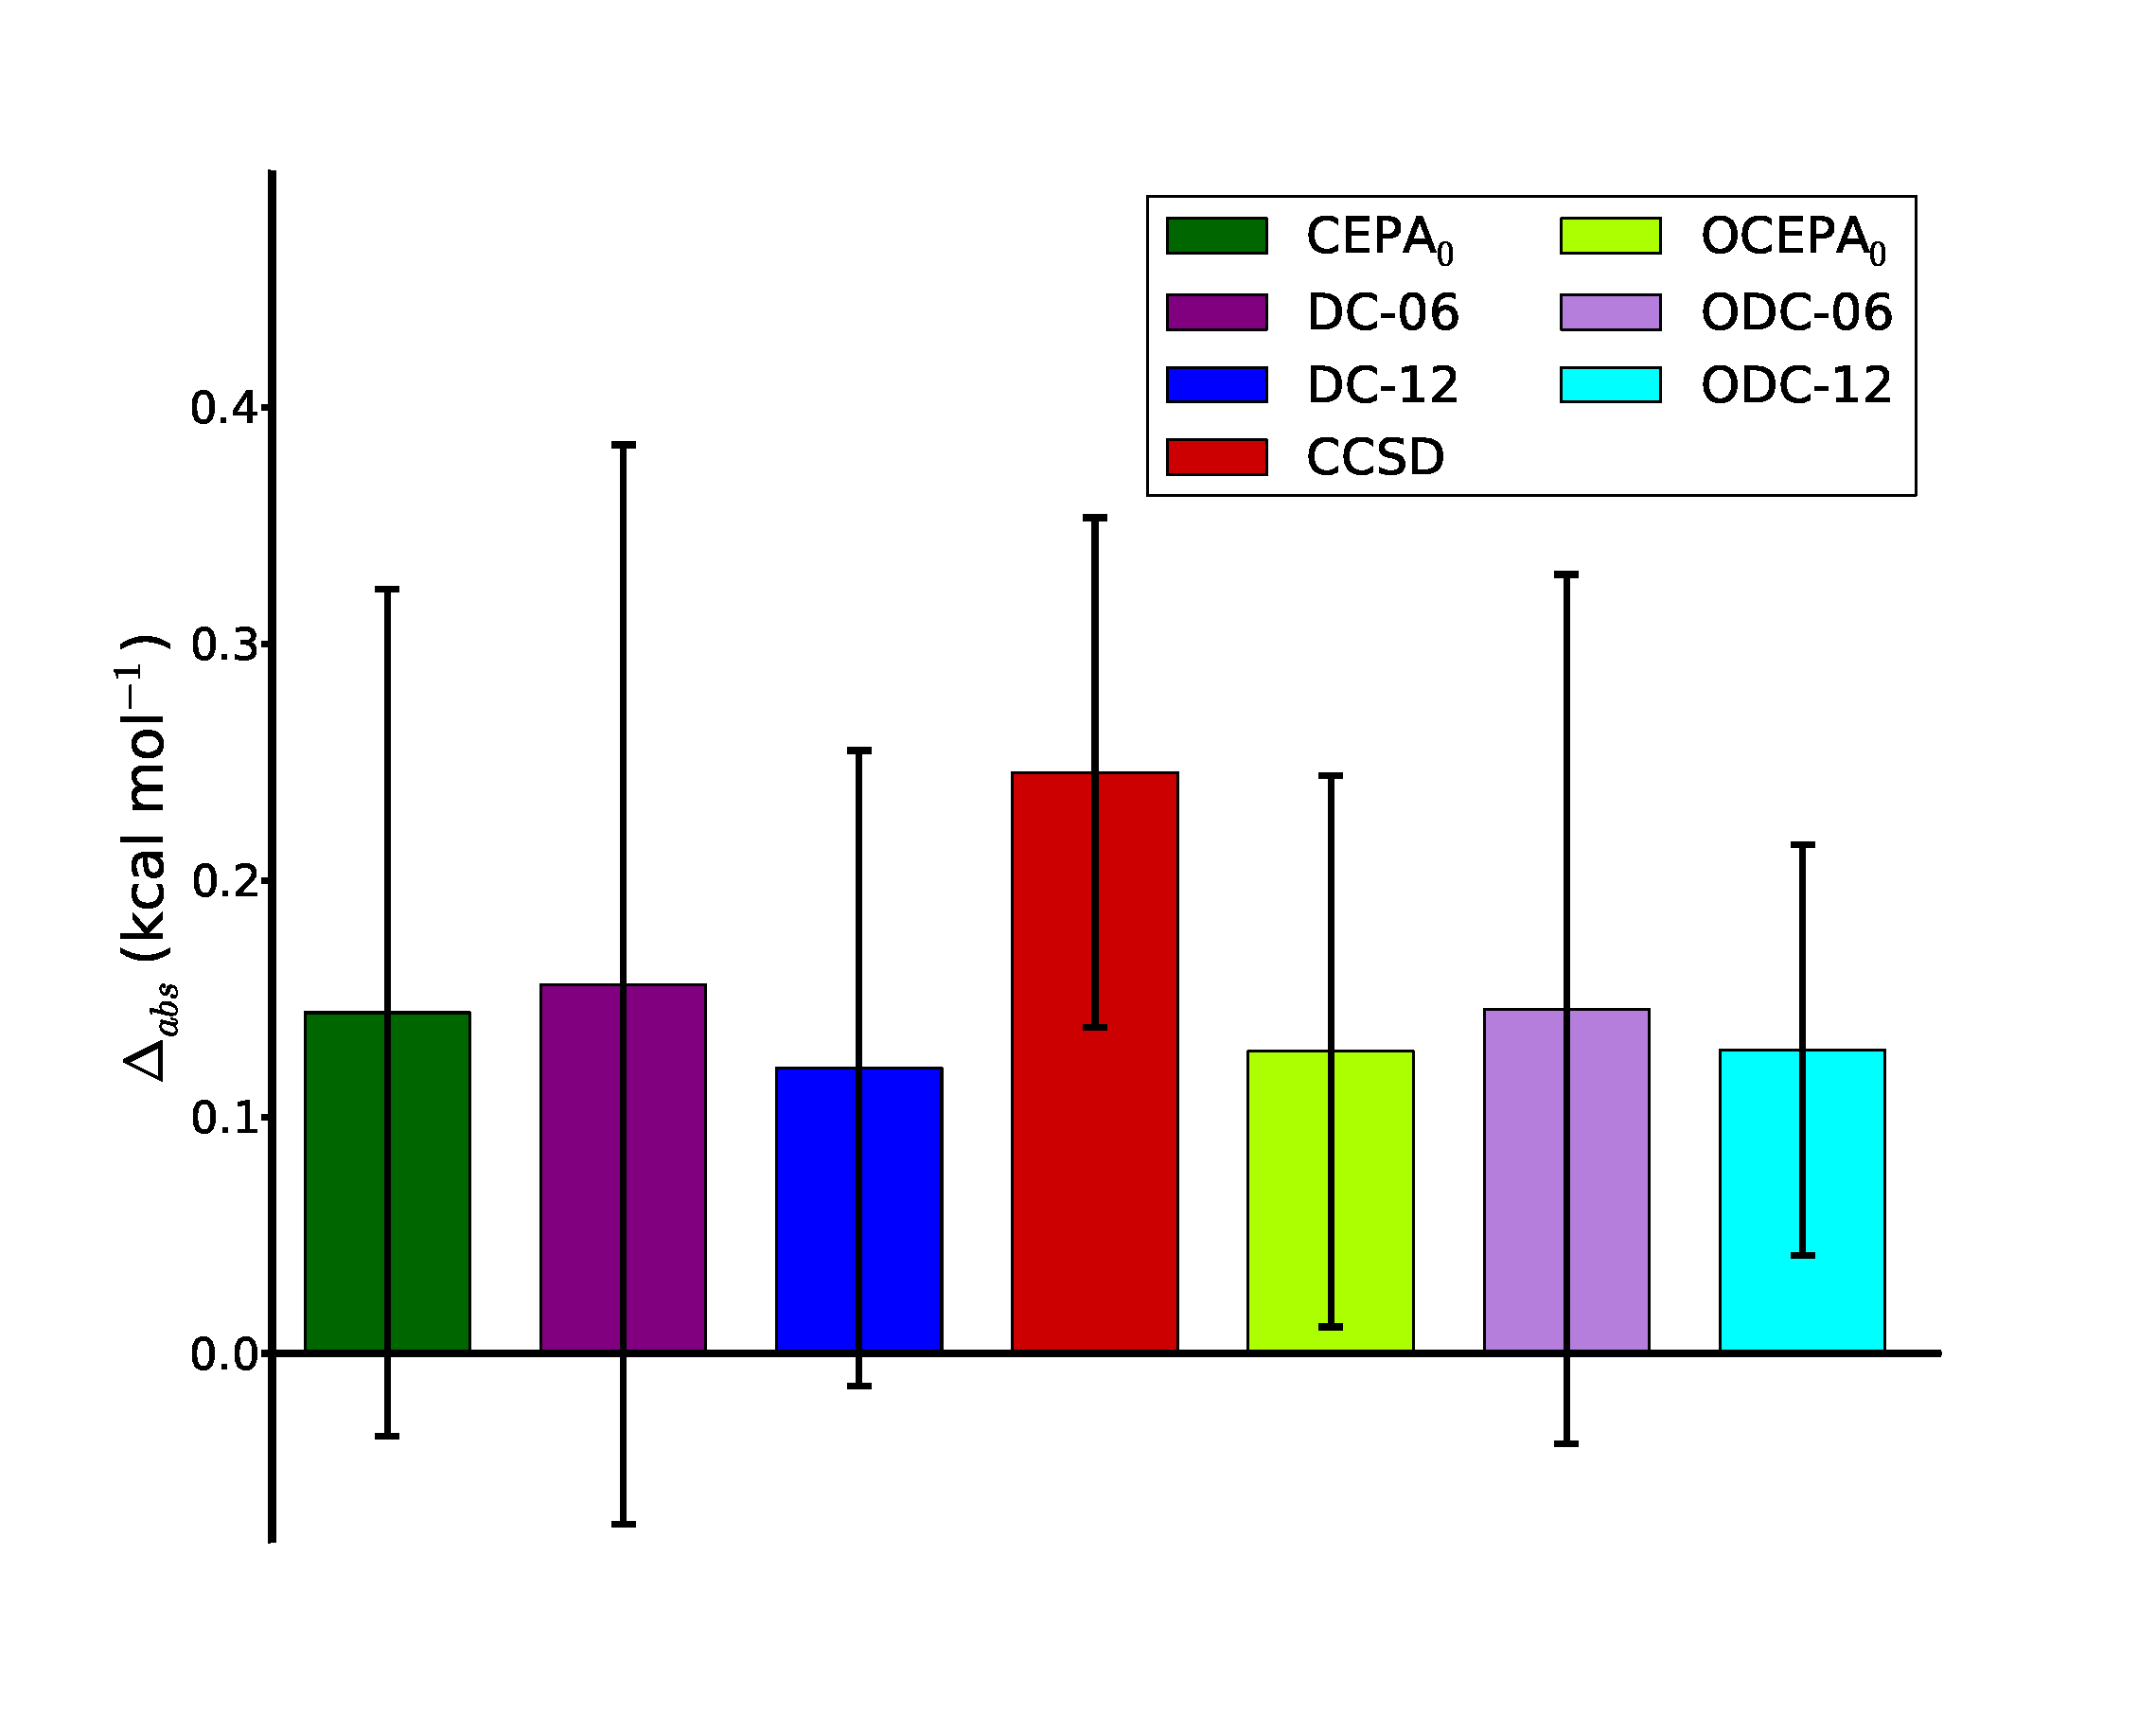
\includegraphics[width=0.8\textwidth]{figures/a24.pdf}
    \captionof{figure}{%
        \label{a24-f}
        Mean absolute deviations (\mae, \kcal) and the standard deviations
        from the mean signed error (\std, \kcal) of the interaction energies
        for 24 noncovalently bound molecular dimers (A24 database) computed
        using seven methods with the aug-cc-pVTZ basis set.
        The errors are relative to CCSD(T)/aug-cc-pVTZ reference values.
        The \mae value is represented as a height of each colored box, while
        the \std value is depicted as a radius of the black vertical bar.
        See \cref{a24-t} for data on individual database members.
    }
}


We begin by testing the accuracy of DCFT methods for the description of
noncovalent interactions in 24 closed-shell molecular dimers, which are listed
in \cref{a24-t}.
These molecular complexes comprise the A24 dataset\cite{Rezac:2013p2151}
developed by \v{R}ez\'a\v{c} and Hobza to include a variety of noncovalent
interactions, including hydrogen bonding and $\pi$-$\pi$ stacking.
Although \v{R}ez\'a\v{c} and Hobza reported the interaction energies at the
CCSD(T) complete basis set (CBS) limit, we use CCSD(T)/aug-cc-pVTZ energies as
reference values in order to effectively exclude basis-set incompleteness error
from the comparison.

\Cref{a24-f} depicts mean absolute error (\mae) relative to CCSD(T) in the
binding energies of CEPA$_0$, OCEPA$_0$, CCSD, and the four DCFT methods (DC-06,
DC-12, ODC-06, and ODC-12), as well as the root mean square deviation from the
average signed error (\std).
All methods but CCSD give similar \mae values ($0.14\pm 0.02$~\kcal), and a
comparison between CEPA$_0$, DC-06, and DC-12 and their orbital-optimized
variants (OCEPA$_0$, ODC-06, and ODC-12) shows negligible 0.01~\kcal differences
in each case.
CCSD gives a significantly larger \mae (0.25~\kcal) than the other methods,
exceeding the DC-12 \mae by a factor of two (0.12~\kcal).
The \std values are much more sensitive to the choice of method than the \mae
values, and are noticeably affected by orbital optimization.
ODC-12 gives the smallest standard deviation (\std = 0.09~\kcal), while the
largest \std value was found for DC-06 (0.23~\kcal). The OCEPA$_0$, ODC-06, and
ODC-12 methods (\std = 0.12, 0.18, and 0.09~\kcal, respectively) exhibit much
more consistent performance than their non-orbital-optimized analogues, with
\std smaller by $0.05\pm 0.01$~\kcal in each case.
CCSD also exhibits a relatively small \std value ($0.11$~\kcal), possibly due to
its inclusion of single excitations which partly account for orbital relaxation.

Errors in interaction energy and CCSD(T) reference values for each molecular
complex are shown in \cref{a24-t}.
The largest deviations from CCSD(T) were obtained for the formaldehyde dimer
($\mathrm{CH_2O }\cdots\mathrm{CH_2O }$, complex 9 in \cref{a24-t}), for which
DC-06, CEPA$_0$, and OCEPA$_0$ yield errors of 0.99, 0.89, and 0.87~\kcal,
respectively.
For this system, the best performance is shown by CCSD and ODC-12, both of which
give an error of 0.46~\kcal.
For systems with $\pi$-stacking interactions (complexes 22-24 in \cref{a24-t}),
CCSD shows large errors (0.38, 0.43, 0.34~\kcal) relative to the magnitude of
the interaction energy (0.43, 0.41, 0.91~\kcal, respectively).
Here CEPA$_0$, DC-12, and their orbital-optimized variants offer much better
agreement with CCSD(T), with errors ranging from 0.01 to 0.15 \kcal.


\subsection{Hydrogen-Transfer Reaction Barrier Heights}

\afterpage{%
    \clearpage
    \centering
    \begin{landscape}
        \vspace*{\fill}
        \captionof{table}{%
            \label{htbh-t}
            Errors in barrier heights (\kcal) for 18 hydrogen-transfer
            reactions (\ce{R1 + R2H $\rightarrow$ R1H + R2}) comprising the
            HTBH38 database\cite{MN-Database} computed using five methods
            with the aug-cc-pVTZ basis set.
            The errors are relative to CCSD(T) reference values (\kcal)
            shown in the rightmost column.
            Each reaction includes barrier heights in the forward (\ce{R1 +
            R2H $\rightarrow$ [R1R2H]^*}) and reverse (\ce{[R1R2H]^*
            $\leftarrow$ R1H + R2}) directions, respectively, except in the
            case of \(\ce{R1} = \ce{R2} = H\) where they are the same.
            The mean absolute (\mae, \kcal) and the mean percent (\rel, \%)
            errors with respect to CCSD(T), as well as the standard
            deviations from the mean signed error (\std, \kcal) are also
            shown.
        }
        \vspace{1em}
        \renewcommand\arraystretch{0.6}
        \begin{tabular}{lcrrrrrr}
            \hline
            \hline
            &
            Reaction Barrier &
            $\Delta$CEPA$_0$ &  $\Delta$DC-12 &   $\Delta$CCSD &
            $\Delta$OCEPA$_0$ & $\Delta$ODC-12 &
            CCSD(T)
            \\
            \hline
            1 & \ce{H + HCl  $\rightarrow$ [HHCl]^*} &
            0.74 & 0.49 & 0.09 & -0.41 & -0.28 & 5.22 \\
            2 &\ce{OH + H2  $\rightarrow$ [OHH2]^*} &
            3.77 & 3.38 & 1.82 & 0.88 & 1.24 & 4.99 \\
            3 &\ce{CH3 + H2  $\rightarrow$ [CH3H2]^*} &
            1.60 & 1.46 & 1.37 & 0.46 & 0.70 & 11.29 \\
            4 &\ce{OH + CH4  $\rightarrow$ [OHCH4]^*} &
            4.26 & 3.85 & 2.61 & 1.22 & 1.65 & 5.64 \\
            5 &\ce{H + H2  $\rightarrow$ [HH2]^*} &
            0.80 & 0.69 & 0.30 & -0.27 & -0.05 & 9.77 \\
            6 &\ce{OH + NH3  $\rightarrow$ [OHNH3]^*} &
            6.02 & 5.25 & 3.54 & 1.18 & 1.82 & 3.17 \\
            7 &\ce{HCl + CH3  $\rightarrow$ [HClCH3]^*} &
            1.93 & 1.78 & 1.79 & 0.68 & 0.92 & 0.10 \\
            8 &\ce{OH + C2H6  $\rightarrow$ [OHC2H6]^*}
            & 4.66 & 4.21 & 2.69 & 1.28 & 1.72 & 2.69 \\
            9 &\ce{F + H2  $\rightarrow$ [FH2]^*} &
            3.40 & 3.14 & 1.20 & 0.52 & 0.78 & 1.13 \\
            10 &\ce{O + CH4  $\rightarrow$ [OHCH3]^*} &
            3.40 & 3.12 & 2.37 & 0.70 & 1.20 & 13.62 \\
            11 &\ce{H + PH3  $\rightarrow$ [HPH3]^*} &
            0.93 & 0.86 & 0.59 & -0.16 & 0.10 & 2.29 \\
            12 &\ce{H + HO  $\rightarrow$ [OHH]^*} &
            2.03 & 1.59 & 0.44 & -0.61 & -0.26 & 10.25 \\
            13 &\ce{H + H2S  $\rightarrow$ [HH2S]^*} &
            1.01 & 0.92 & 0.65 & -0.11 & 0.14 & 3.17 \\
            14 &\ce{O + HCl  $\rightarrow$ [OHCl]^*} &
            6.33 & 6.01 & 3.58 & 0.79 & 1.51 & 9.74 \\
            15 &\ce{NH2 + CH3  $\rightarrow$ [CH3NH2]^*} &
            2.48 & 2.22 & 1.99 & 0.49 & 0.86 & 7.66 \\
            16 &\ce{NH2 + C2H5  $\rightarrow$ [NH2C2H5]^*} &
            2.48 & 2.22 & 2.09 & 0.55 & 0.92 & 8.21 \\
            17 &\ce{C2H6 + NH2  $\rightarrow$ [C2H6NH2]^*} &
            3.30 & 3.00 & 2.73 & 1.23 & 1.62 & 10.39 \\
            18 &\ce{NH2 + CH4  $\rightarrow$ [NH2CH4]^*} &
            2.98 & 2.72 & 2.55 & 1.11 & 1.48 & 13.23 \\
            \hline
        \end{tabular}
        \vspace*{\fill}
        \newpage
        \vspace*{\fill}
        \begin{tabular}{lcrrrrrr}
            \hline
            \hline
            &
            Reaction Barrier &
            $\Delta$CEPA$_0$ &  $\Delta$DC-12 &   $\Delta$CCSD &
            $\Delta$OCEPA$_0$ & $\Delta$ODC-12 &
            CCSD(T)
            \\
            \hline
            1 & \ce{[HHCl]^* $\leftarrow$  H2 + Cl} &
            1.44 & 1.31 & 1.61 & 0.53 & 0.77 & 7.39 \\
            2 &\ce{[OHH2]^* $\leftarrow$  H + H2O} &
            2.09 & 1.66 & 0.09 & -0.91 & -0.58 & 21.07 \\
            3 &\ce{[CH3H2]^* $\leftarrow$  H + CH4} &
            0.95 & 0.80 & 0.38 & -0.38 & -0.11 & 14.91 \\
            4 &\ce{[OHCH4]^* $\leftarrow$  CH3 + H2O} &
            3.23 & 2.80 & 1.87 & 0.27 & 0.65 & 18.09 \\
            6 &\ce{[OHNH3]^* $\leftarrow$  H2O + NH2} &
            5.46 & 4.62 & 3.14 & 0.79 & 1.33 & 13.17 \\
            7 &\ce{[HClCH3]^* $\leftarrow$  Cl + CH4} &
            1.97 & 1.94 & 2.31 & 0.78 & 1.16 & 5.89 \\
            8 &\ce{[OHC2H6]^* $\leftarrow$  H2O + C2H5} &
            3.34 & 2.89 & 1.85 & 0.28 & 0.64 & 18.49 \\
            9 &\ce{[FH2]^* $\leftarrow$  HF + H} &
            1.27 & 0.88 & -0.78 & -1.47 & -1.33 & 32.95 \\
            10 &\ce{[OHCH3]^* $\leftarrow$  OH + CH3} &
            2.62 & 2.29 & 1.82 & 0.32 & 0.68 & 7.43 \\
            11 &\ce{[HPH3]^* $\leftarrow$  PH2 + H2} &
            1.14 & 1.11 & 1.37 & 0.39 & 0.63 & 23.21 \\
            12 &\ce{[OHH]^* $\leftarrow$  H2 + O} &
            3.47 & 3.08 & 1.99 & 0.62 & 1.07 & 12.81 \\
            13 &\ce{[HH2S]^* $\leftarrow$  H2 + HS} &
            1.51 & 1.51 & 1.88 & 0.65 & 0.97 & 16.41 \\
            14 &\ce{[OHCl]^* $\leftarrow$  OH + Cl} &
            5.59 & 5.35 & 3.55 & 0.51 & 1.24 & 9.35 \\
            15 &\ce{[CH3NH2]^* $\leftarrow$  CH4 + NH} &
            2.77 & 2.49 & 2.26 & 0.73 & 1.12 & 21.32 \\
            16 &\ce{[NH2C2H5]^* $\leftarrow$  C2H6 + NH} &
            3.06 & 2.75 & 2.46 & 0.85 & 1.26 & 18.52 \\
            17 &\ce{[C2H6NH2]^* $\leftarrow$  NH3 + C2H5} &
            2.54 & 2.30 & 2.30 & 0.63 & 1.02 & 16.20 \\
            18 &\ce{[NH2CH4]^* $\leftarrow$  CH3 + NH3} &
            2.51 & 2.29 & 2.21 & 0.56 & 0.96 & 15.69
            \\
            \hline
            &
            \mae: &
            2.77 & 2.49 & 1.84 & 0.67 & 0.94 &
            \\
            &
            \std: &
            1.51 & 1.39 & 1.06 & 0.62 & 0.71 &
            \\
            &
            \rel \%: &
            99 & 90 & 77 & 29 & 40
            \\
            \hline
            \hline
        \end{tabular}
        \vspace*{\fill}
    \end{landscape}
    \newpage
    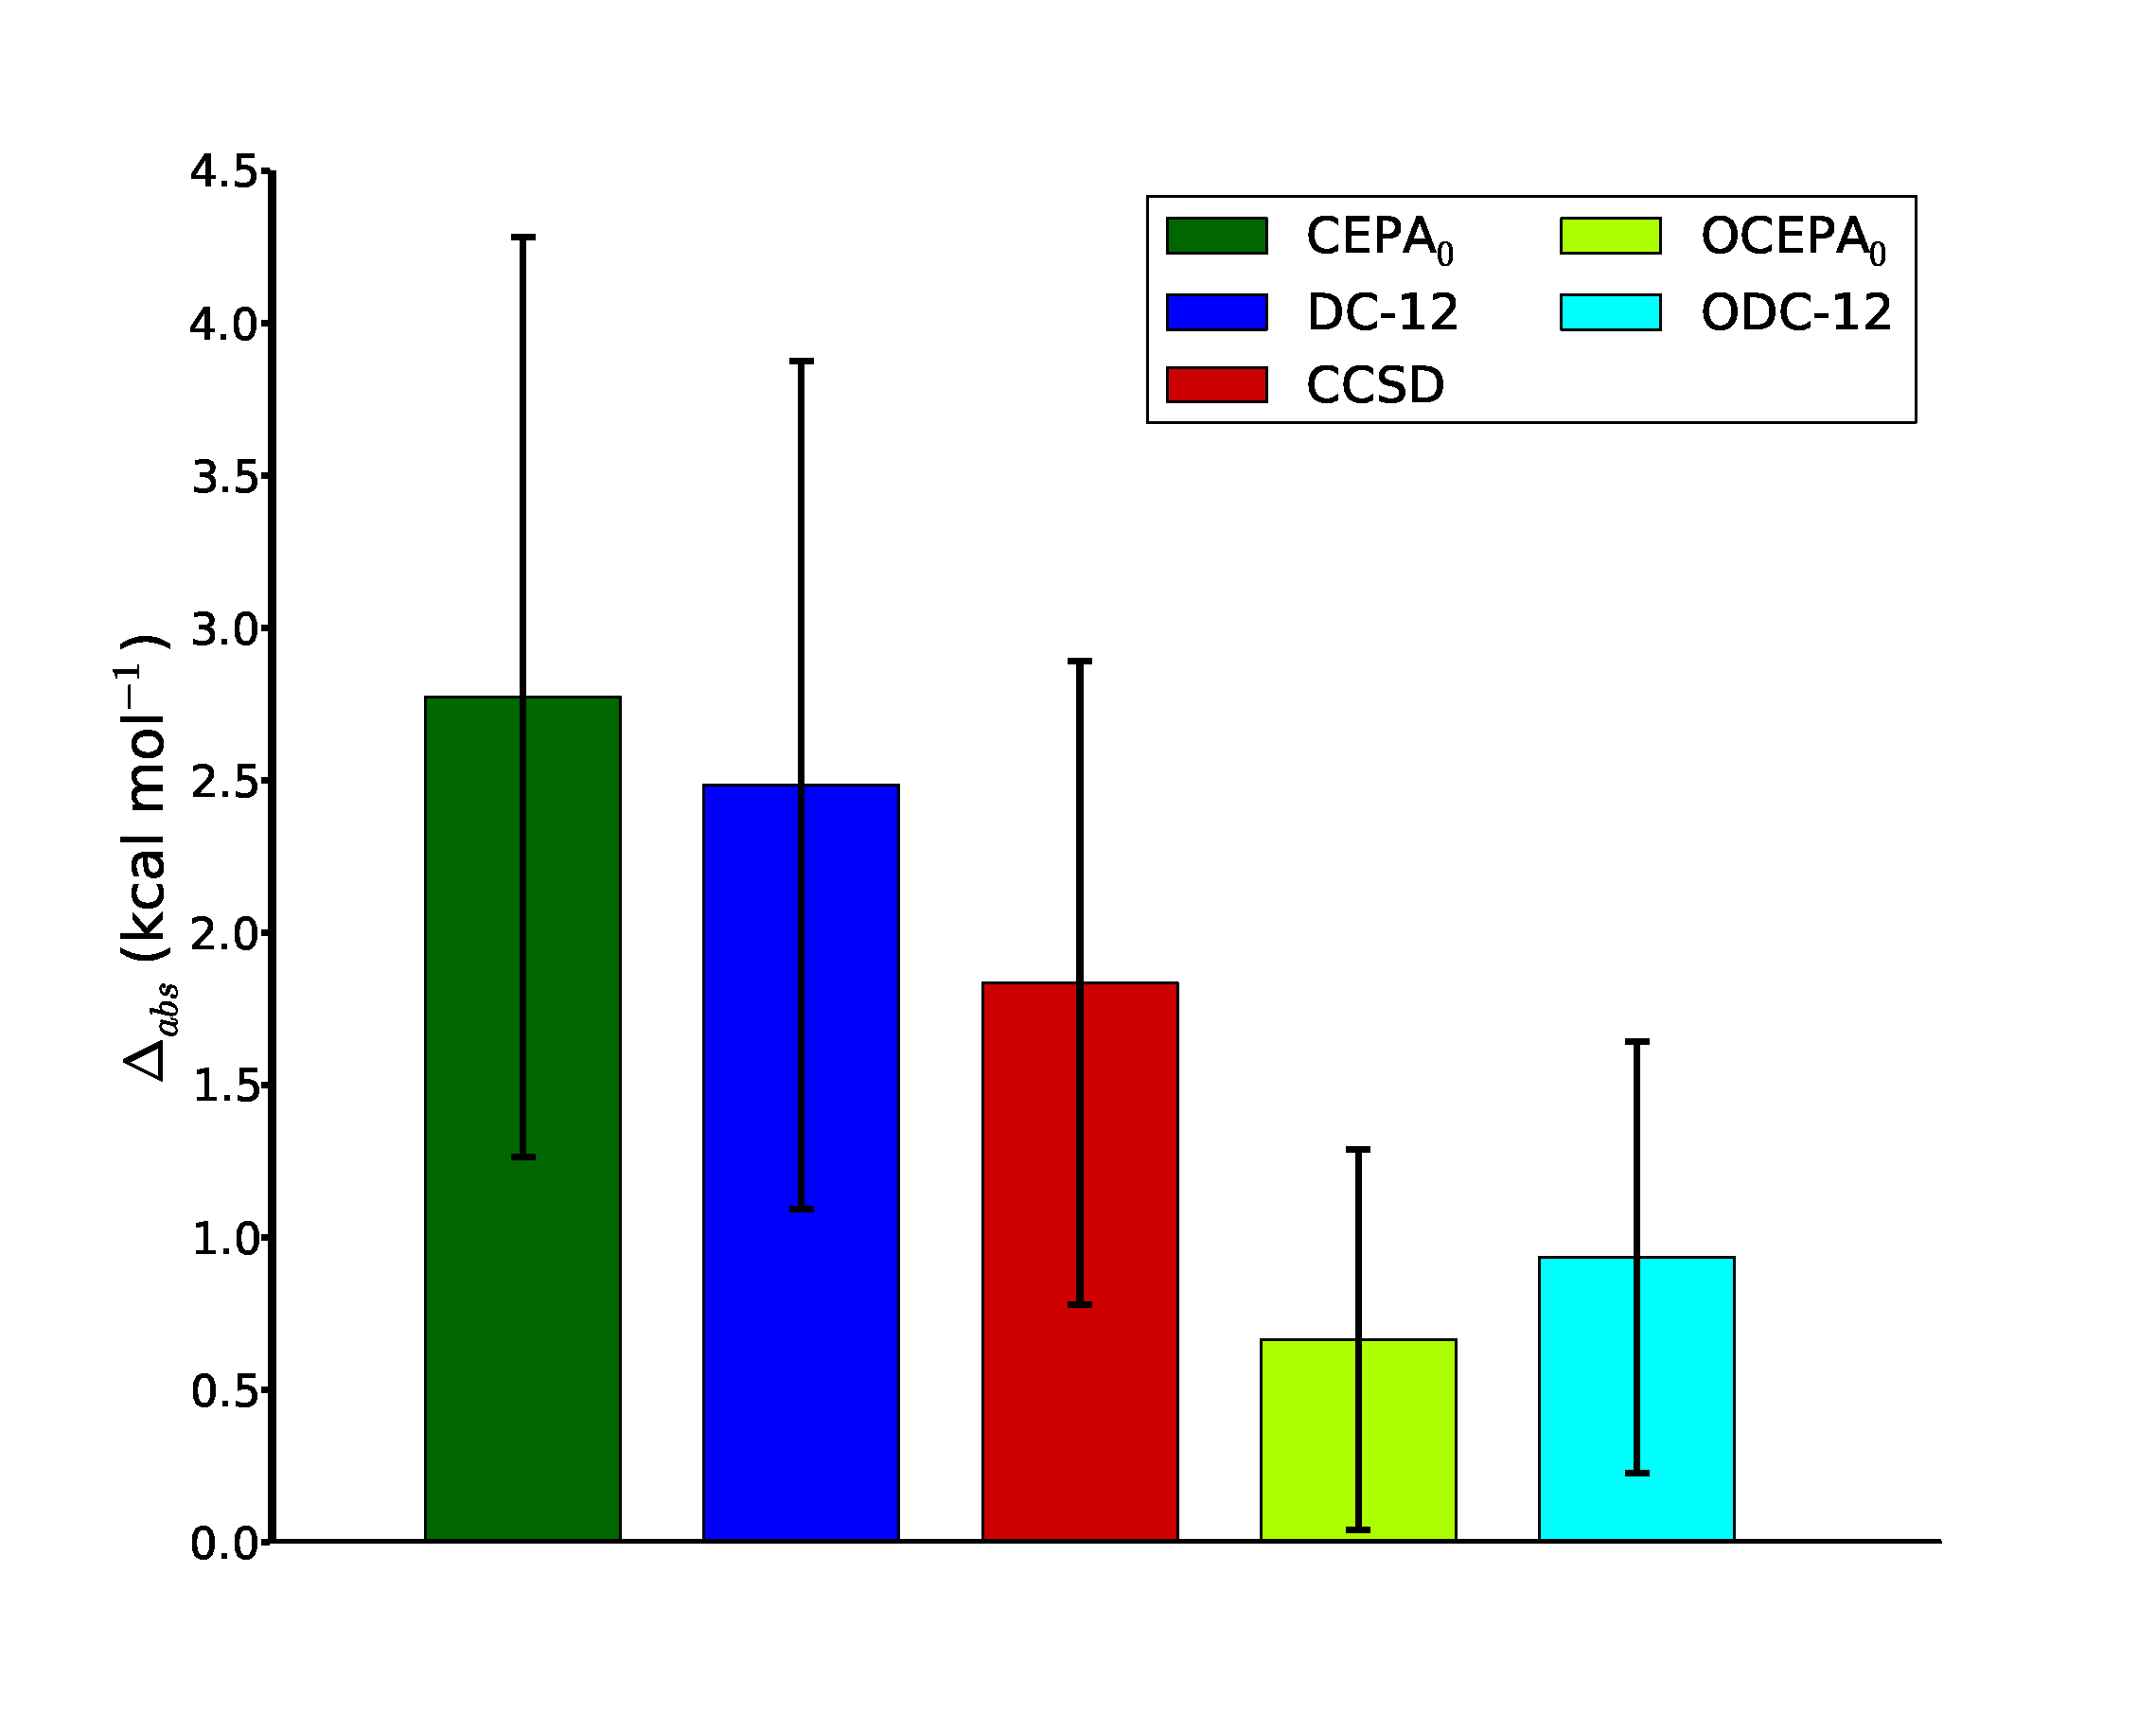
\includegraphics[width=0.8\textwidth]{figures/htbh.pdf}
    \captionof{figure}{%
        \label{htbh-f}
        Mean absolute deviations (\mae, \kcal) and the standard deviations
        from the mean signed error (\std, \kcal) of barrier heights for 18
        hydrogen-transfer reactions (\ce{R1 + R2H $\rightarrow$ R1H + R2},
        HTBH38 database) computed using five methods with the aug-cc-pVTZ
        basis set.
        The errors are relative to CCSD(T)/aug-cc-pVTZ reference values.
        The \mae value is represented as a height of each colored box, while
        the \std value is depicted as a radius of the black vertical bar.
        See \cref{htbh-t} for data on individual database members.
    }
}

We continue by assessing the performance of DCFT methods in predicting barrier
heights for 18 hydrogen-transfer reactions from the HTBH38
database:\cite{Zhao:2005p43}
\begin{equation}
    \ce{R1 + R2H -> [R1R2H]^* -> R1H + R2}
\end{equation}
These reactions\footnote{Reaction 19 in HTBH38, the cis-trans isomerization of
piperylene, is omitted in the present study.} involve molecules ($\mathrm{R_1}$
and $\mathrm{R_2}$) and transition states ($\mathrm{[R_1R_2H]^*}$) with
open-shell character, making their properties more sensitive to electron
correlation effects. 
We employ barrier heights computed at the CCSD(T)/aug-cc-pVTZ level of theory as
our reference rather than the values provided by Lynch\cite{MN-Database} in
order to effectively exclude basis-set incompleteness effects. We also omit the
DC-06 and ODC-06 methods, which encounter frequent convergence problems due to
the poor description of $N$-representability (see Supporting Information for
incomplete DC-06 results).

Mean absolute deviations (\mae) and standard deviations (\std) for the
hydrogen-transfer barrier heights are presented in \cref{htbh-t} and plotted in
\cref{htbh-f}.
The largest \mae values come from CEPA$_0$ and DC-12 (2.77 and 2.49~\kcal,
respectively).
Orbital optimization greatly improves the accuracy of these methods, resulting
in \mae values of just 0.67 and 0.94~\kcal for OCEPA$_0$ and ODC-12,
respectively.
The CCSD method shows intermediate performance with \mae = 1.84~\kcal.
A similar trend is observed for the \std values, with OCEPA$_0$ (0.62~\kcal) and
ODC-12 (0.71~\kcal) significantly improving upon CEPA$_0$ (1.51~\kcal), DC-12
(1.39~\kcal), and CCSD (1.06~\kcal).
In addition to \mae and \std, \cref{htbh-t} includes mean percent error (\rel)
values, which are commonly used to benchmark performance for reaction kinetics.
The smallest \rel values are 29\% and 40\% for OCEPA$_0$ and ODC-12,
respectively.

Turning to barrier heights for individual hydrogen-transfer reactions
(\cref{htbh-t}), the largest errors are observed for reactions 6 and 14, both
involving the OH radical, for which CEPA$_0$ and DC-12 give errors of $\sim$
5-6~\kcal.
The best results for these reactions are obtained from OCEPA$_0$, with errors
ranging from 0.51 to 1.18~\kcal.
The ODC-12 method tends to predict larger barrier heights than OCEPA$_0$,
yielding smaller errors only when OCEPA$_0$ underestimates the barrier heights.

\subsection{Radical Stabilization Energies}

\afterpage{%
    \clearpage
    \centering
    \begin{landscape}
        \vspace*{\fill}
        \captionof{table}{%
            \label{rse-t}
            Errors in radical stabilization energies (RSEs, \kcal) for 30
            open-shell doublet species (\ce{{}^.R}) comprising the RSE30
            database \cite{Soydas:2013p1452} computed using six methods with
            the cc-pCVTZ basis set.
            The errors are relative to CCSD(T) with an added quadruples
            correction ($\delta Q = E_\mathrm{CCSDT(Q)}-E_\mathrm{CCSD(T)}$)
            shown in the rightmost column in \kcal.
            The $\delta$Q correction was computed using the cc-pCVDZ basis
            set.  RSE is defined as the reaction enthalpy for the
            homodesmotic reaction \ce{{}^.CH3 + RH $\rightarrow$ CH4 +
            {}^.R}.
            To indicate the degree of spin-contamination in the UHF
            reference, the spin expectation values
            ($\langle\hat{\mathsf{S}}^2\rangle_{\text{SCF}}$) are also shown
            in units of $\hbar^2$.
            For each method the mean absolute deviations from
            CCSD(T)${+}\delta$Q (\mae, \kcal) and the standard deviations
            from the mean signed error (\std, \kcal) are also presented.
        }
        \vspace{1em}
        \renewcommand\arraystretch{0.6}
        \small
        \begin{tabular}{llrrrrrrrr}
            \hline
            \hline
            \ce{{}^.R} & \(\langle\hat{S}^2\rangle_\mathrm{SCF}\) &
            \(\Delta\)CEPA$_0$ & \(\Delta\)DC-12 & \(\Delta\)CCSD &
            \(\Delta\)OCEPA$_0$ & \(\Delta\)ODC-12 & \(\Delta\)CCSD(T) &
            CCSD(T){+}\(\delta\)Q
            \\
            \hline
            \ce{{}^.CH2NO2} &
            0.78  & 1.24 & 0.95 & 0.66 & 0.16 & 0.27 & 0.32 &
            -3.50 \\ 
            \ce{{}^.CH2OCHO} &
            0.76  & 1.16 & 1.12 & 0.63 & 0.40 & 0.48 & 0.10 &
            -4.84 \\
            \ce{{}^.CH2SCH3} &
            0.76  & 1.89 & 1.70 & 0.81 & 0.63 & 0.72 & 0.15 &
            -11.01 \\
            \ce{{}^.CF\bond{2}CH2} &
            0.94  & 6.12 & 3.71 & 0.96 & 0.42 & 0.64 & 0.46 &
            6.26 \\
            \ce{{}^.CH2CH2F} &
            0.76  & 0.30 & 0.27 & 0.13 & 0.08 & 0.10 & 0.04 &
            -1.53 \\
            \ce{{}^.CH2CHO} &
            0.93  & 5.01 & 2.86 & 0.32 & -0.16 & 0.02 & 0.46 &
            -10.11\\
            \ce{{}^.CH2CN} &
            0.94  & 6.36 & 3.52 & 0.65 & -0.02 & 0.21 & 0.46 &
            -8.66 \\
            \ce{{}^.CH2F} &
            0.76  & 1.03 & 1.00 & 0.52 & 0.55 & 0.57 & 0.06 &
            -4.22 \\
            \ce{{}^.CH2NH2} &
            0.76  & 1.28 & 1.18 & 0.59 & 0.50 & 0.52 & 0.06 &
            -12.06\\
            \ce{{}^.CH2NH3+} &
            0.76  & 0.16 & 0.10 & 0.08 & 0.06 & 0.03 & 0.02 &
            4.58 \\
            \ce{{}^.CH2NHOH} &
            0.77  & 1.76 & 1.57 & 0.78 & 0.58 & 0.64 & 0.15 &
            -8.81 \\
            \ce{{}^.CH2OH} &
            0.76  & 1.29 & 1.23 & 0.62 & 0.57 & 0.60 & 0.07 &
            -9.27 \\
            \ce{{}^.CH2PH3+} &
            0.76 & 0.21 & 0.14 & 0.01 & 0.01 & -0.02 & 0.05 &
            0.49 \\
            \ce{{}^.CH2SH2+} &
            0.77 & 0.41 & 0.30 & 0.12 & 0.11 & 0.08 & 0.06 &
            2.29 \\
            \ce{{}^.CH2SH} &
            0.76 & 1.60 & 1.43 & 0.68 & 0.57 & 0.63 & 0.12 &
            -9.68 \\
            \hline
        \end{tabular}
        \vspace*{\fill}
        \newpage
        \vspace*{\fill}
        \begin{tabular}{lllrrrrrrr}
            \hline
            \hline
            \ce{{}^.R} & \(\langle\hat{S}^2\rangle_\mathrm{SCF}\) &
            \(\Delta\)CEPA$_0$ & \(\Delta\)DC-12 & \(\Delta\)CCSD &
            \(\Delta\)OCEPA$_0$ & \(\Delta\)ODC-12 & \(\Delta\)CCSD(T) &
            CCSD(T){+}\(\delta\)Q
            \\
            \hline
            \ce{{}^.CH2C\bond{3}CH} &
            1.00  & 6.23 & 3.47 & 0.82 & -0.03 & 0.23 & 0.52 &
            -13.17\\
            \ce{{}^.CH2CH3} &
            0.76  & 0.30 & 0.26 & 0.11 & 0.08 & 0.10 & 0.03 &
            -3.36 \\
            \ce{{}^.CH2Cl} &
            0.77 & 1.13 & 1.02 & 0.50 & 0.48 & 0.51 & 0.09 &
            -5.67 \\
            \ce{{}^.CH2BH2} &
            0.76 & 0.17 & 0.17 & 0.05 & 0.03 & 0.04 & 0.05 &
            -11.66\\
            \ce{{}^.CHO} &
            0.77  & 2.26 & 2.24 & 1.48 & 1.55 & 1.56 & 0.20 &
            -17.61\\
            \ce{{}^.CH2PH2} &
            0.76 & 1.17 & 1.02 & 0.39 & 0.36 & 0.39 & 0.12 &
            -6.50 \\
            \ce{{}^.CHClF} &
            0.76  & 1.61 & 1.52 & 0.76 & 0.78 & 0.81 & 0.13 &
            -6.61 \\
            \ce{{}^.CHFCH3} &
            0.76 & 1.07 & 1.01 & 0.50 & 0.51 & 0.53 & 0.08 &
            -5.87 \\
            \ce{{}^.CH(OH)2} &
            0.76 & 1.30 & 1.22 & 0.60 & 0.60 & 0.61 & 0.08 &
            -6.67 \\
            \ce{{}^.CHCl2} &
            0.77 & 1.78 & 1.57 & 0.72 & 0.72 & 0.75 & 0.15 &
            -9.56 \\
            \ce{{}^.CHF2} &
            0.76 & 1.50 & 1.48 & 0.78 & 0.83 & 0.85 & 0.10 &
            -4.07 \\
            \ce{CH2\bond{2}C^.\bond{1}CN} &
            1.39 & 19.10 & 11.50 & 2.36 & -0.31 & 0.29 & 1.80 &
            1.98 \\
            \ce{{}^.C\bond{3}CH} &
            1.15 & 11.20 & 6.51 & 0.77 & -0.78 & -0.07 & 0.82 &
            26.25 \\
            \ce{{}^.CH\bond{2}CH2} &
            0.94 & 5.42 & 3.01 & 0.58 & 0.11 & 0.31 & 0.40 &
            5.49 \\
            \ce{{}^.CH2\bond{1}CH\bond{2}CH2} &
            0.97 & 4.98 & 3.17 & 0.51 & 0.11 & 0.31 & 0.48 &
            -17.53 \\
            \hline
            &&
            \mae: &
            2.97 & 2.01 & 0.62 & 0.40 & 0.43 & 0.25	&
            \\
            &&
            \std: &
            3.97 & 2.27 & 0.45 & 0.43 & 0.35 & 0.35	&
            \\
            \hline
            \hline
        \end{tabular}
        \vspace*{\fill}
    \end{landscape}
    \newpage
    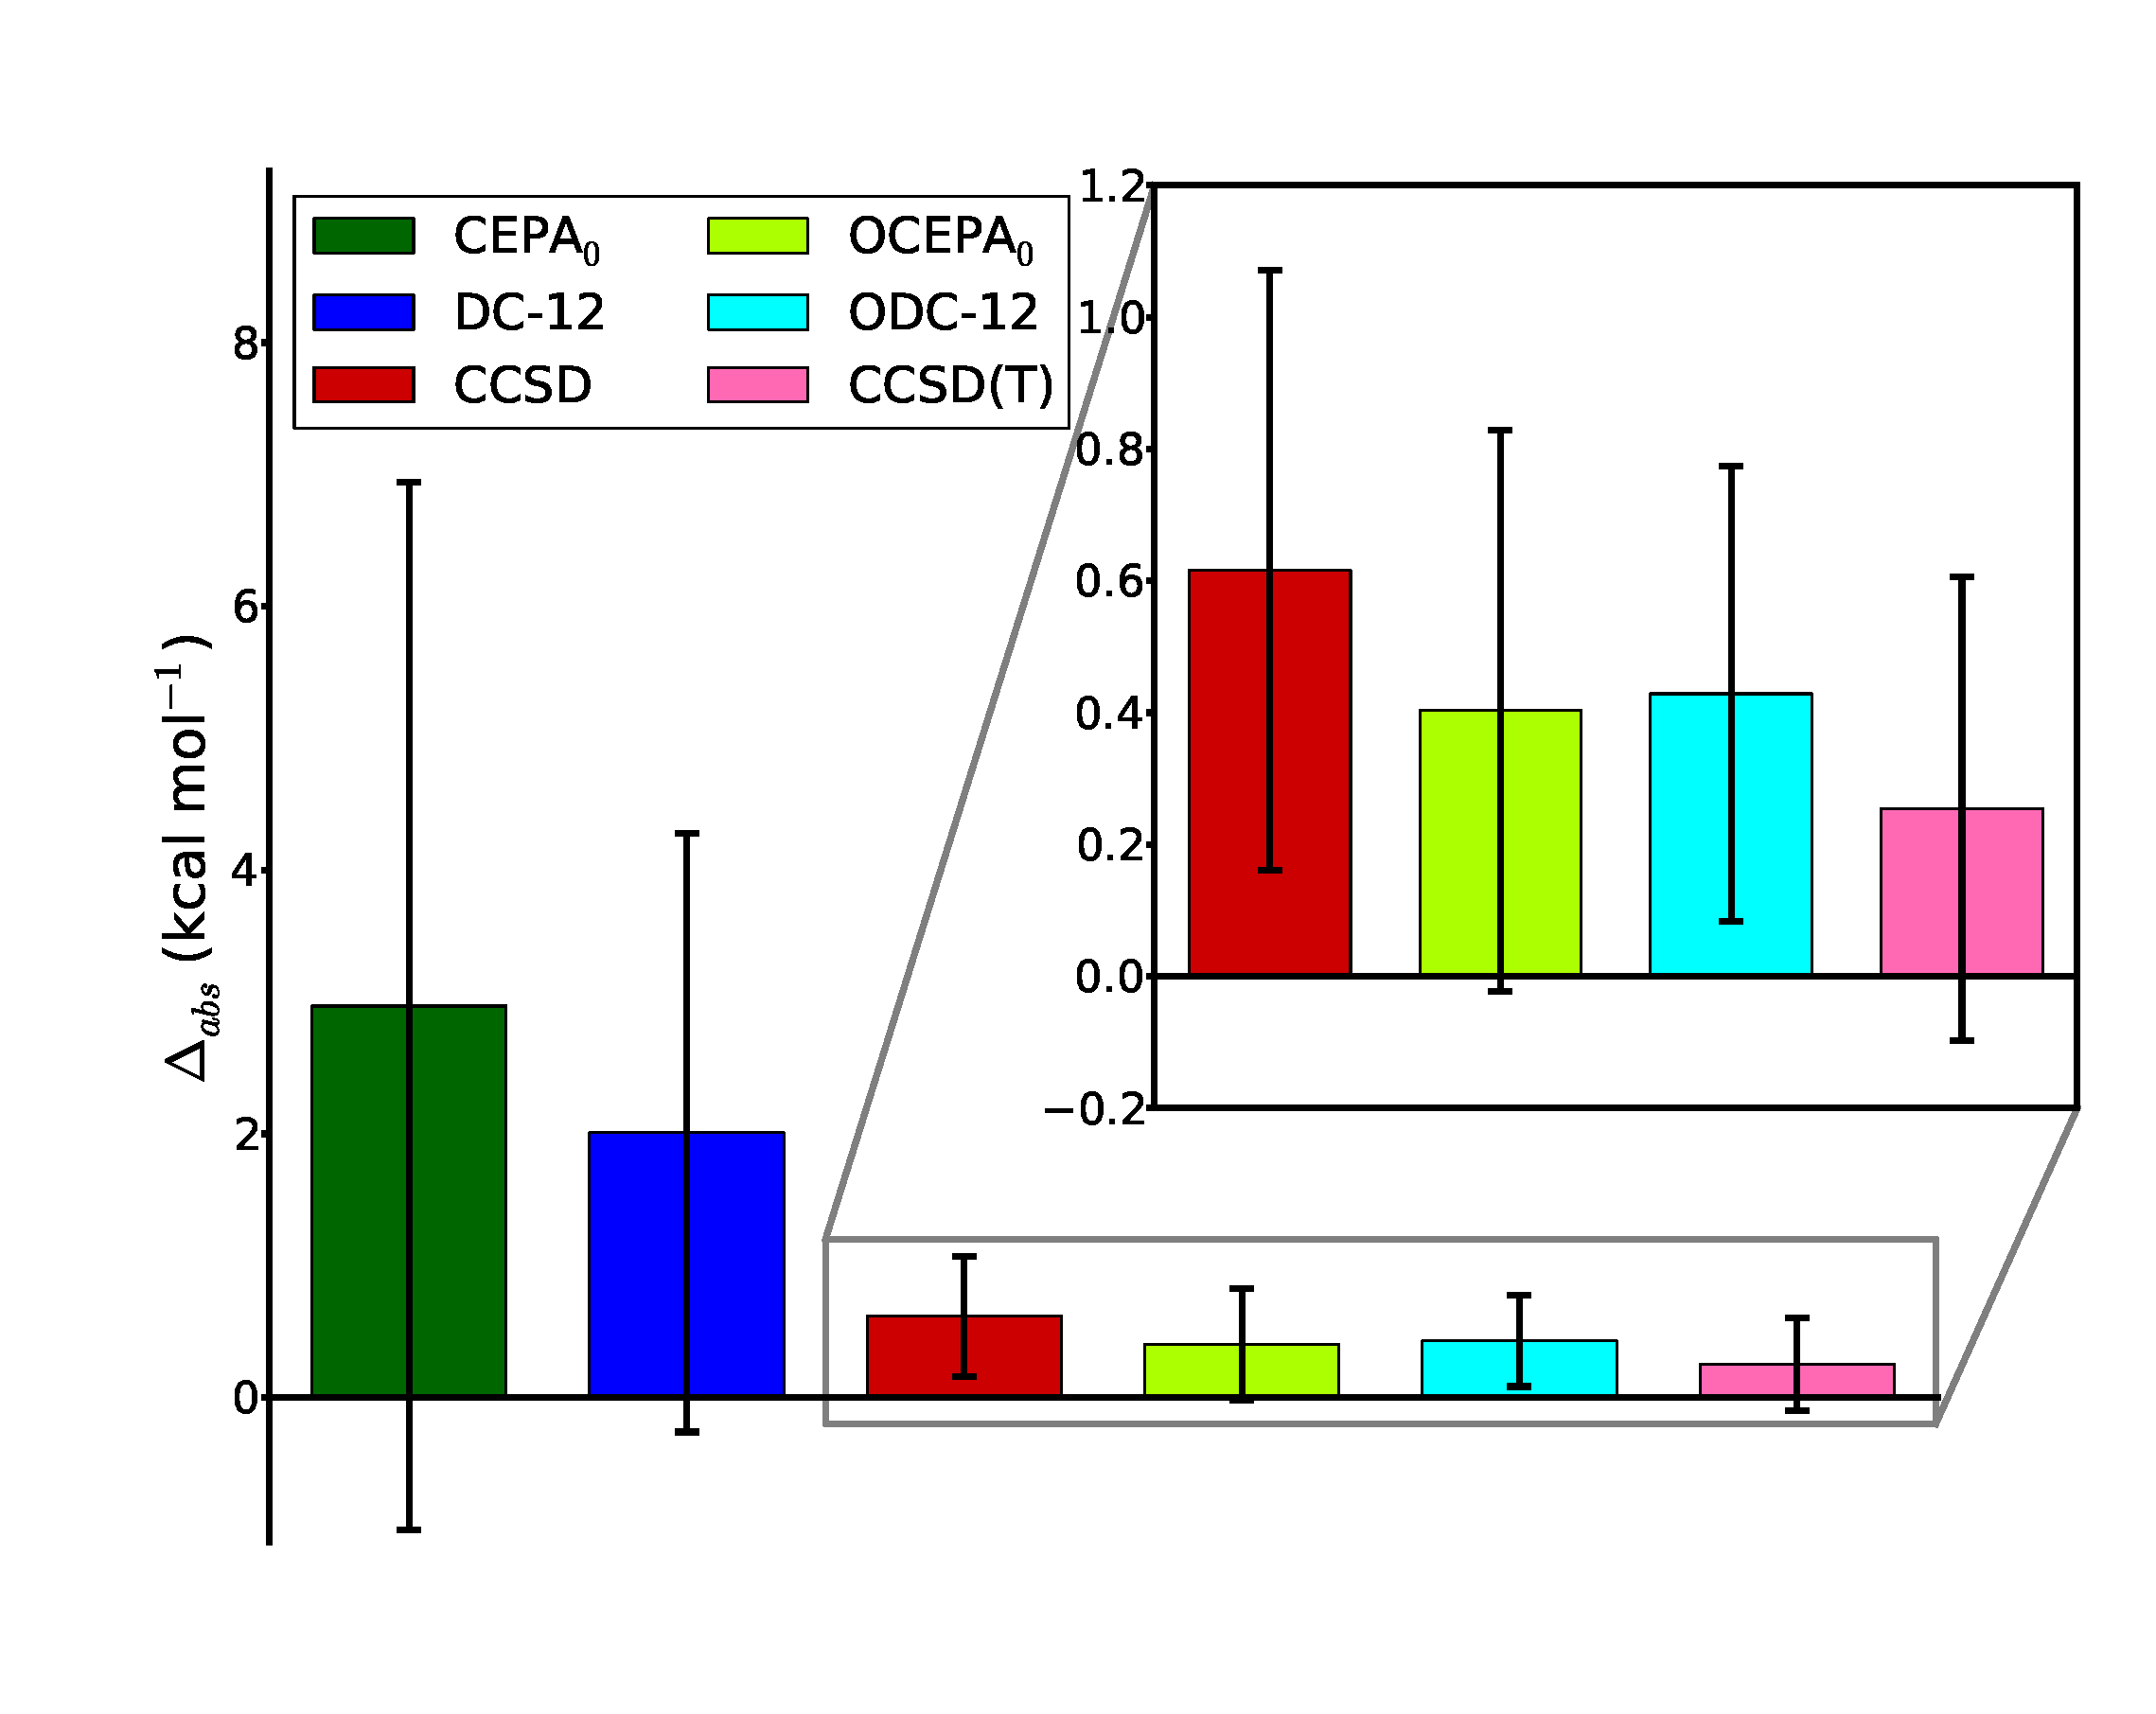
\includegraphics[width=0.8\textwidth]{figures/rse.pdf}
    \captionof{figure}{%
        \label{rse-f}
        Mean absolute deviations (\mae, \kcal) and the standard deviations
        from the mean signed error (\std, \kcal) of the radical
        stabilization energies (RSEs) for 30 open-shell doublet species
        (RSE30 database) computed using six methods with the cc-pCVTZ basis
        set.
        The errors are relative to CCSD(T) with an added quadruples
        correction ($\delta$Q  $= E_\mathrm{CCSDT(Q)}-E_\mathrm{CCSD(T)}$).
        The $\delta$Q correction was computed using the cc-pCVDZ basis set.
        RSE is defined as the reaction enthalpy for the homodesmotic
        reaction \ce{{}^.CH3 + RH $\rightarrow$ CH4 + {}^.R}.
        The \mae value is represented as a height of each colored box, while
        the \std value is depicted as a radius of the black vertical bar.
        See \cref{rse-t} for data on individual database members.
    }
}

In this section we study the performance of DCFT methods for predicting radical
stabilization energies (RSEs). An R-group's RSE is defined as the enthalpy of a
homodesmotic reaction
\begin{equation}
    \ce{%
        RH
        +
        {}^.CH3
        ->
        {}^.R
        +
        CH4
    }
\end{equation}
where exothermic (negative) values indicate that the radical \ce{{}^.R} is more
thermodynamically stable than \ce{{}^.CH3}.\cite{Zipse:2006p163}
For our benchmark we use the RSE30 dataset\cite{Soydas:2013p1452}, which
provides a diverse variety of \ce{{}^.R} species (listed in \cref{rse-t}).
Since the performance of CCSD(T) is known to deteriorate for strongly
spin-contaminated UHF
references,\cite{Byrd:2001p9736,Beran:2003p2488,Lochan:2007p164101,Kurlancheek:2009p1223,Bozkaya:2011p224103}
we augment CCSD(T) energies with a quadruples correction ($\Delta$Q  =
$E_\mathrm{CCSDT(Q)}-E_\mathrm{CCSD(T)}$) and use these as our benchmark.
CBS-extrapolated CCSD(T) reference values have been published for this
dataset,\cite{Soydas:2014p1073} but we use CCSD(T) values computed with the
cc-pCVTZ basis set to avoid basis-set incompleteness effects. 
The $\delta$Q correction was evaluated using the cc-pCVDZ basis set. 
As in the previous Section, DC-06 and ODC-06 computations cannot be converged
for all database members and are omitted in the analysis below (see Supporting
Information for incomplete DC-06 and ODC-06 data).


The relative performance of the DCFT, CEPA, and CC methods for the RSE30 dataset
is shown in \cref{rse-f}.
The effect of orbital-optimization on accuracy is now even more pronounced,
reducing the large \mae errors of CEPA$_0$ (2.97~\kcal) and DC-12 (2.01~\kcal)
to 0.40 and 0.43~\kcal for OCEPA$_0$ and ODC-12, respectively. CCSD has a
slightly larger \mae value (0.62~\kcal), while CCSD(T) has the smallest overall
\mae (0.25~\kcal).
Both CEPA$_0$ and DC-12 show large standard deviations again (3.97 and
2.27~\kcal, respectively).
For OCEPA$_0$, the standard deviation (0.43~\kcal) is similar to that of CCSD
(0.45~\kcal). ODC-12 and CCSD(T) exhibit the most consistent performance with
the same \std value of 0.35~\kcal.

Deviations from CCSD(T){+}\(\delta\)Q for individual RSEs predicted by each
method are tabulated in \cref{rse-t}.
In addition, \cref{rse-t} includes expectation values of the square-norm spin
operator computed for the UHF wavefunction of \ce{{}^.R}
($\langle\hat{S}^2\rangle_\mathrm{SCF}$).
The largest errors in computed RSEs were obtained for \ce{{}^.R} species with
\(
    \langle\hat{S}^2\rangle_\mathrm{SCF}
    >
    0.9\
    \hbar^2
\)
(radicals 4, 6, 7, 16, and 27-30 in \cref{rse-t}).
For these systems, the average CEPA$_0$ and DC-12 errors are 8.05 and
4.72~\kcal, and the average CCSD(T) error is 0.68~\kcal.
OCEPA$_0$ and ODC-12 offer remarkably better performance for this subset, with
average errors of 0.24~\kcal and 0.26~\kcal.


\afterpage{%
    \clearpage
    \centering
    \begin{landscape}
        \vspace*{\fill}
        \captionof{table}{%
            \label{ip-t}
            Errors in adiabatic ionization energies (AIEs, \eV) for 10 di-
            and triatomic molecules computed using six methods with the
            cc-pCVQZ basis set.
            The errors are relative to experimental values
            (\(\mathrm{IE}_\mathrm{ref}\), \eV) from
            Ref.~\citenum{Lias:1988p1}, unless noted otherwise.
            For all AIEs the harmonic zero-point vibrational energy
            corrections were included.
            For each method the mean absolute deviations from
            \(\mathrm{IE}_\mathrm{ref}\) (\mae, \eV) and the standard
            deviations from the mean signed error (\std, \eV) are also
            shown.
        }
        \vspace{1em}
        \renewcommand\arraystretch{0.6}
        \small
        \begin{threeparttable}
            \begin{tabular}{ccrrrrrrc}
                \hline
                \hline
                Molecule & Transition &
                $\Delta$CEPA$_0$ &
                $\Delta$DC-12 &
                $\Delta$CCSD &
                $\Delta$OCEPA$_0$ &
                $\Delta$ODC-12 &
                $\Delta$CCSD(T) &
                $\mathrm{IE}_\mathrm{ref}$
                \\
                \hline
                \ce{N2} &
                \(\termsymbol{{}^1\Sigma_g^+}\rightarrow\termsymbol{{}^2\Sigma_g^+}\) &
                0.08 & 0.17 & 0.12 &-0.05 & 0.07 &-0.03 &
                15.581  $\pm$ 0.008 \tnote{a} \\
                \ce{O2} &
                \(\termsymbol{{}^3\Sigma_g^-}\rightarrow\termsymbol{{}^2\Pi_g}\) &
                -0.11 &-0.03 & 0.04 &-0.09 &-0.02 &-0.04 &
                12.0697 $\pm$ 0.0002 \\
                \ce{F2} &
                \(\termsymbol{{}^1\Sigma_g^+}\rightarrow\termsymbol{{}^2\Pi_g}\) &
                0.06 & 0.06 & 0.04 & 0.08 & 0.01 &-0.03	&
                15.697 $\pm$ 0.003 \\
                \ce{NO} &
                \(\termsymbol{{}^2\Pi}\rightarrow\termsymbol{{}^1\Sigma^+}\) &
                -0.15 &-0.05 &-0.05 &-0.05 &-0.02 &-0.09 &
                9.26438 $\pm$ 0.00005 \\
                \ce{OF} &
                \(\termsymbol{{}^2\Pi}\rightarrow\termsymbol{{}^3\Sigma^-}\) &
                0.11 & 0.12 &-0.10 &-0.03 &-0.02 &-0.11	&
                12.77 $\pm$ 0.01 \tnote{b} \\
                \ce{HNC} &
                \(\termsymbol{{}^1\Sigma_g^+}\rightarrow\termsymbol{{}^2\Sigma^+}\) &
                0.27 & 0.14 &-0.12 &-0.14 &-0.08 &-0.04	&
                12.04 $\pm$ 0.01 \tnote{c} \\
                \ce{HOF} &
                \(\termsymbol{{}^1A'}\rightarrow\termsymbol{{}^2A''}\) &
                0.20 & 0.17 &-0.10 &-0.03 &-0.04 &-0.07	&
                12.71 $\pm$ 0.01 \\
                \ce{FNO} &
                \(\termsymbol{{}^1A'}\rightarrow\termsymbol{{}^2A''}\) &
                0.51 & 0.10 &-0.02 &-0.02 &-0.00 & 0.04	&
                12.63 $\pm$ 0.03 \\
                \ce{F2N} &
                \(\termsymbol{{}^2B_1}\rightarrow\termsymbol{{}^1A_1}\) &
                0.07 & 0.10 & 0.07 & 0.01 & 0.03 &-0.08	&
                11.63$\pm$ 0.01 \\
                \ce{F2O} &
                \(\termsymbol{{}^1A_1}\rightarrow\termsymbol{{}^2B_1}\) &
                0.49 & 0.37 &-0.01 & 0.05 & 0.04 &-0.04	&
                13.11 $\pm$ 0.01 \\
                \hline
                & \mae: & 0.21 & 0.13 & 0.06 & 0.05 & 0.03 & 0.06 & \\
                & \std: & 0.22 & 0.12 & 0.08 & 0.06 & 0.04 & 0.04 & \\
                \hline
                \hline
            \end{tabular}
            \begin{tablenotes}
                \item[a]
                    Reference \citenum{Trickl:1989p6006}.
                \item[b]
                    Reference \citenum{Zhang:1994p377}.
                \item[c]
                    Reference \citenum{Hansel:1998p1748}.
            \end{tablenotes}
        \end{threeparttable}
        \vspace*{\fill}
    \end{landscape}
    \newpage
	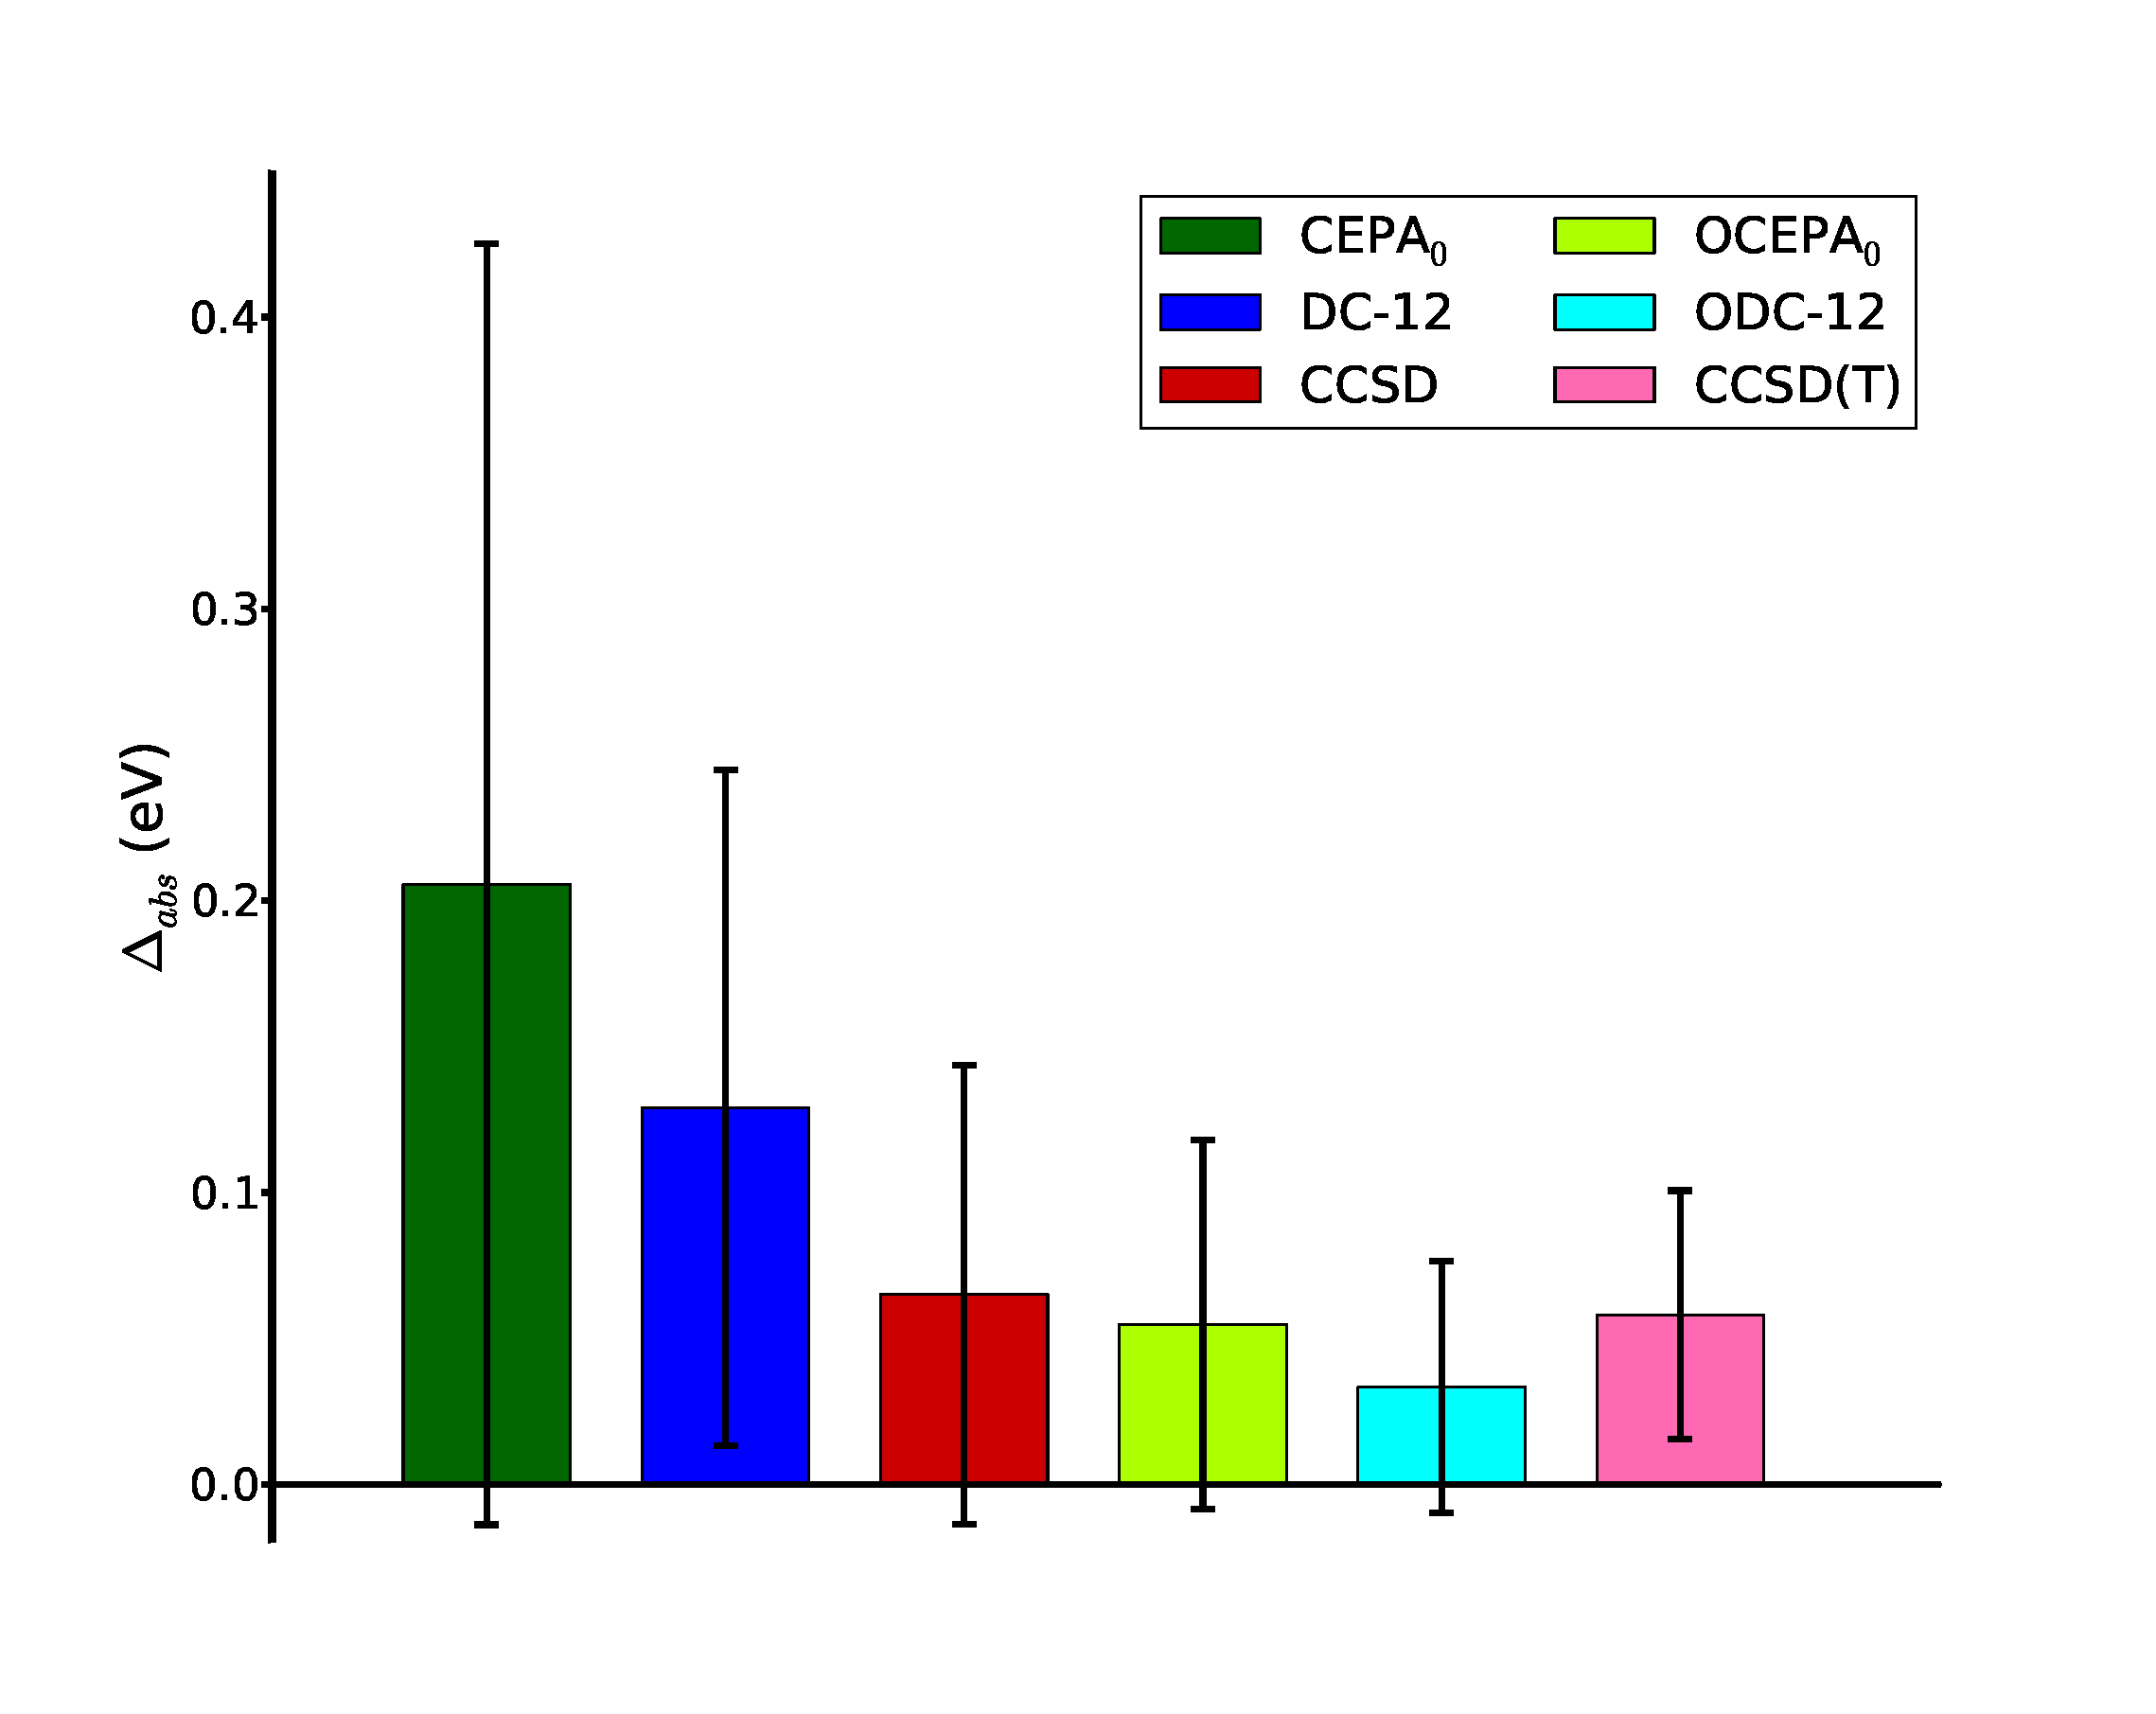
\includegraphics[width=0.8\textwidth]{figures/ip.pdf}
    \captionof{figure}{%
        \label{ip-f}
        Mean absolute deviations (\mae, \eV) and the standard deviations from
        the mean signed error (\std, \eV) of adiabatic ionization energies for
        10 di- and triatomic molecules computed using six methods with the
        cc-pCVQZ basis set.
        The errors are relative to experimental
        values.\cite{Lias:1988p1,Trickl:1989p6006,Zhang:1994p377,Hansel:1998p1748}
        The \mae value is represented as a height of each colored box, while the
        \std value is depicted as a radius of the black vertical bar.
        See \cref{ip-t} for data on individual molecules.
	}
}

\subsection{Adiabatic Ionization Energies in Electron-Dense Molecules}

We conclude the assessment of DCFT methods for the description of thermodynamic
properties by computing adiabatic ionization energies (AIEs) for a set of 10 di-
and triatomic electron-dense molecules (\cref{ip-t}), i.e.\ those that
are composed of elements with small atomic radius, high electron affinity, and
high electronegativity (N, O, F), in order to increase the magnitude of electron
correlation effects.
We use experimentally measured ionization energies reported to high precision
($\sim$0.01~\eV)\cite{Lias:1988p1,Trickl:1989p6006,Zhang:1994p377,Hansel:1998p1748}
as reference values for our benchmark (\(\mathrm{IE}_\mathrm{ref}\),
\cref{ip-t}).
The AIEs were computed using the cc-pCVQZ basis set, with harmonic ZPVE
corrections applied to each neutral and cationic system.

The \mae and \std values for our computed AIEs relative to experiment are
plotted in \cref{ip-f}.
Of the six methods, CEPA$_0$ and DC-12 exhibit the largest \mae values (0.21 and
0.13~\eV, respectively).
The closest agreement with experiment is given by ODC-12, with \mae = 0.03~\eV.
OCEPA$_0$, CCSD, and CCSD(T) show somewhat poorer performance (\mae = 0.05, 0.06
and 0.06~\eV, respectively). 
The \std for ODC-12 matches that of CCSD(T) (0.04~\eV).
For the other methods, the \std values decrease in the order CEPA$_0$ (0.22~\eV)
$>$ DC-12 (0.12) $>$ CCSD (0.08) $>$ OCEPA$_0$ (0.06).

Individual errors for each system are shown in \cref{ip-t}.
Both DC-12 and CEPA$_0$ exhibit large deviations for $\mathrm{F_2O}$ (0.49 and
0.37~\eV), and CEPA$_0$ also gives a large error for FNO (0.51~\eV) which is the
maximum error for this dataset.
Both DC-12 and CEPA$_0$ give errors exceeding 0.1~\eV for seven of the ten
systems, whereas CCSD exhibits errors in excess of 0.1~\eV for only three
systems (OF, HNC, and HOF).
CCSD(T) has only one such error (0.11~\eV for OF), as does OCEPA$_0$ (0.14~\eV
for HNC).
ODC-12 does the best of the methods considered, with a maximum error of
0.08~\eV, found for the AIE of HNC.


\begin{figure}
	\centering
	\caption{%
        \label{bh-f}
        Error in the total energy (\mhartree), relative to full CI, as a
        function of B--H internuclear separation (\AA) computed using six
        methods with the DZP basis set.
        The full CI reference is depicted with a horizontal dotted line.
        The dashed vertical line indicates the full CI equilibrium bond
        distance.
	}
	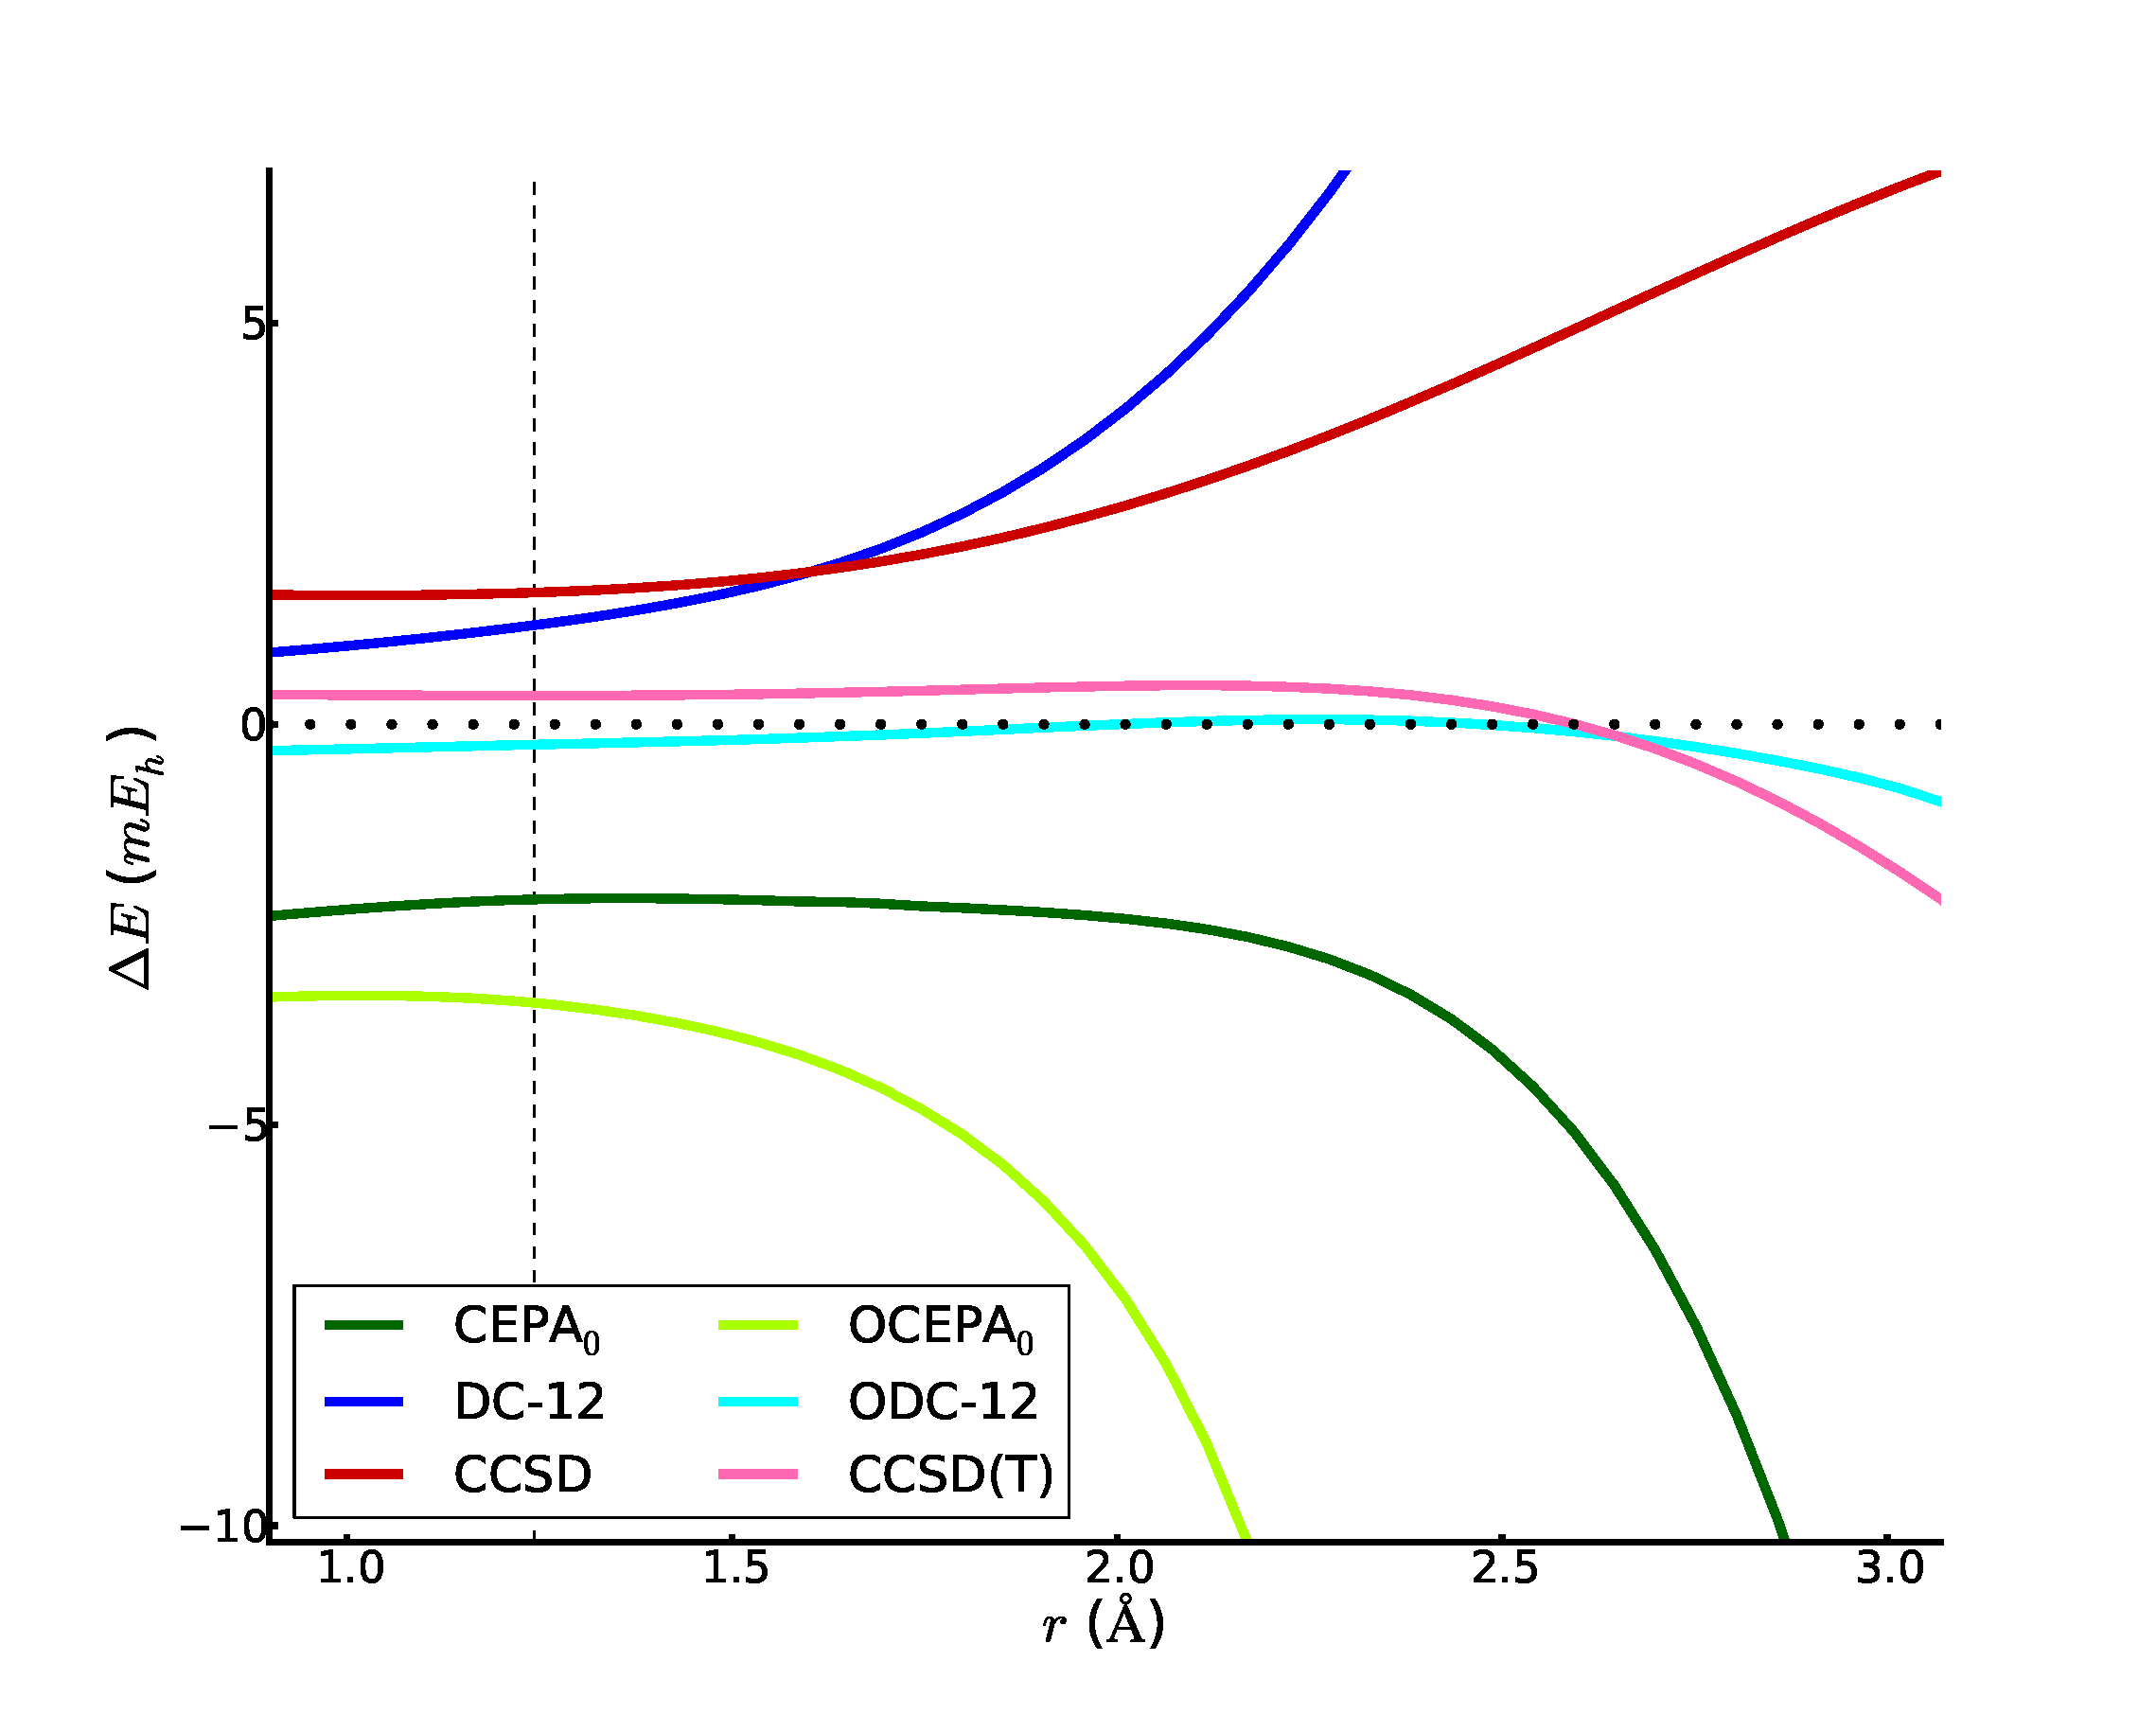
\includegraphics[width=0.8\textwidth]{figures/bh.pdf}
\end{figure}

\begin{figure}
	\centering
	\caption{%
        \label{hf-f}
        Error in the total energy (\mhartree), relative to full CI, as a
        function of H--F internuclear separation (\AA) computed using six
        methods with the DZP basis set.
        The full CI reference is depicted with a horizontal dotted line.
        The dashed vertical line indicates the full CI equilibrium bond
        distance.
	}
	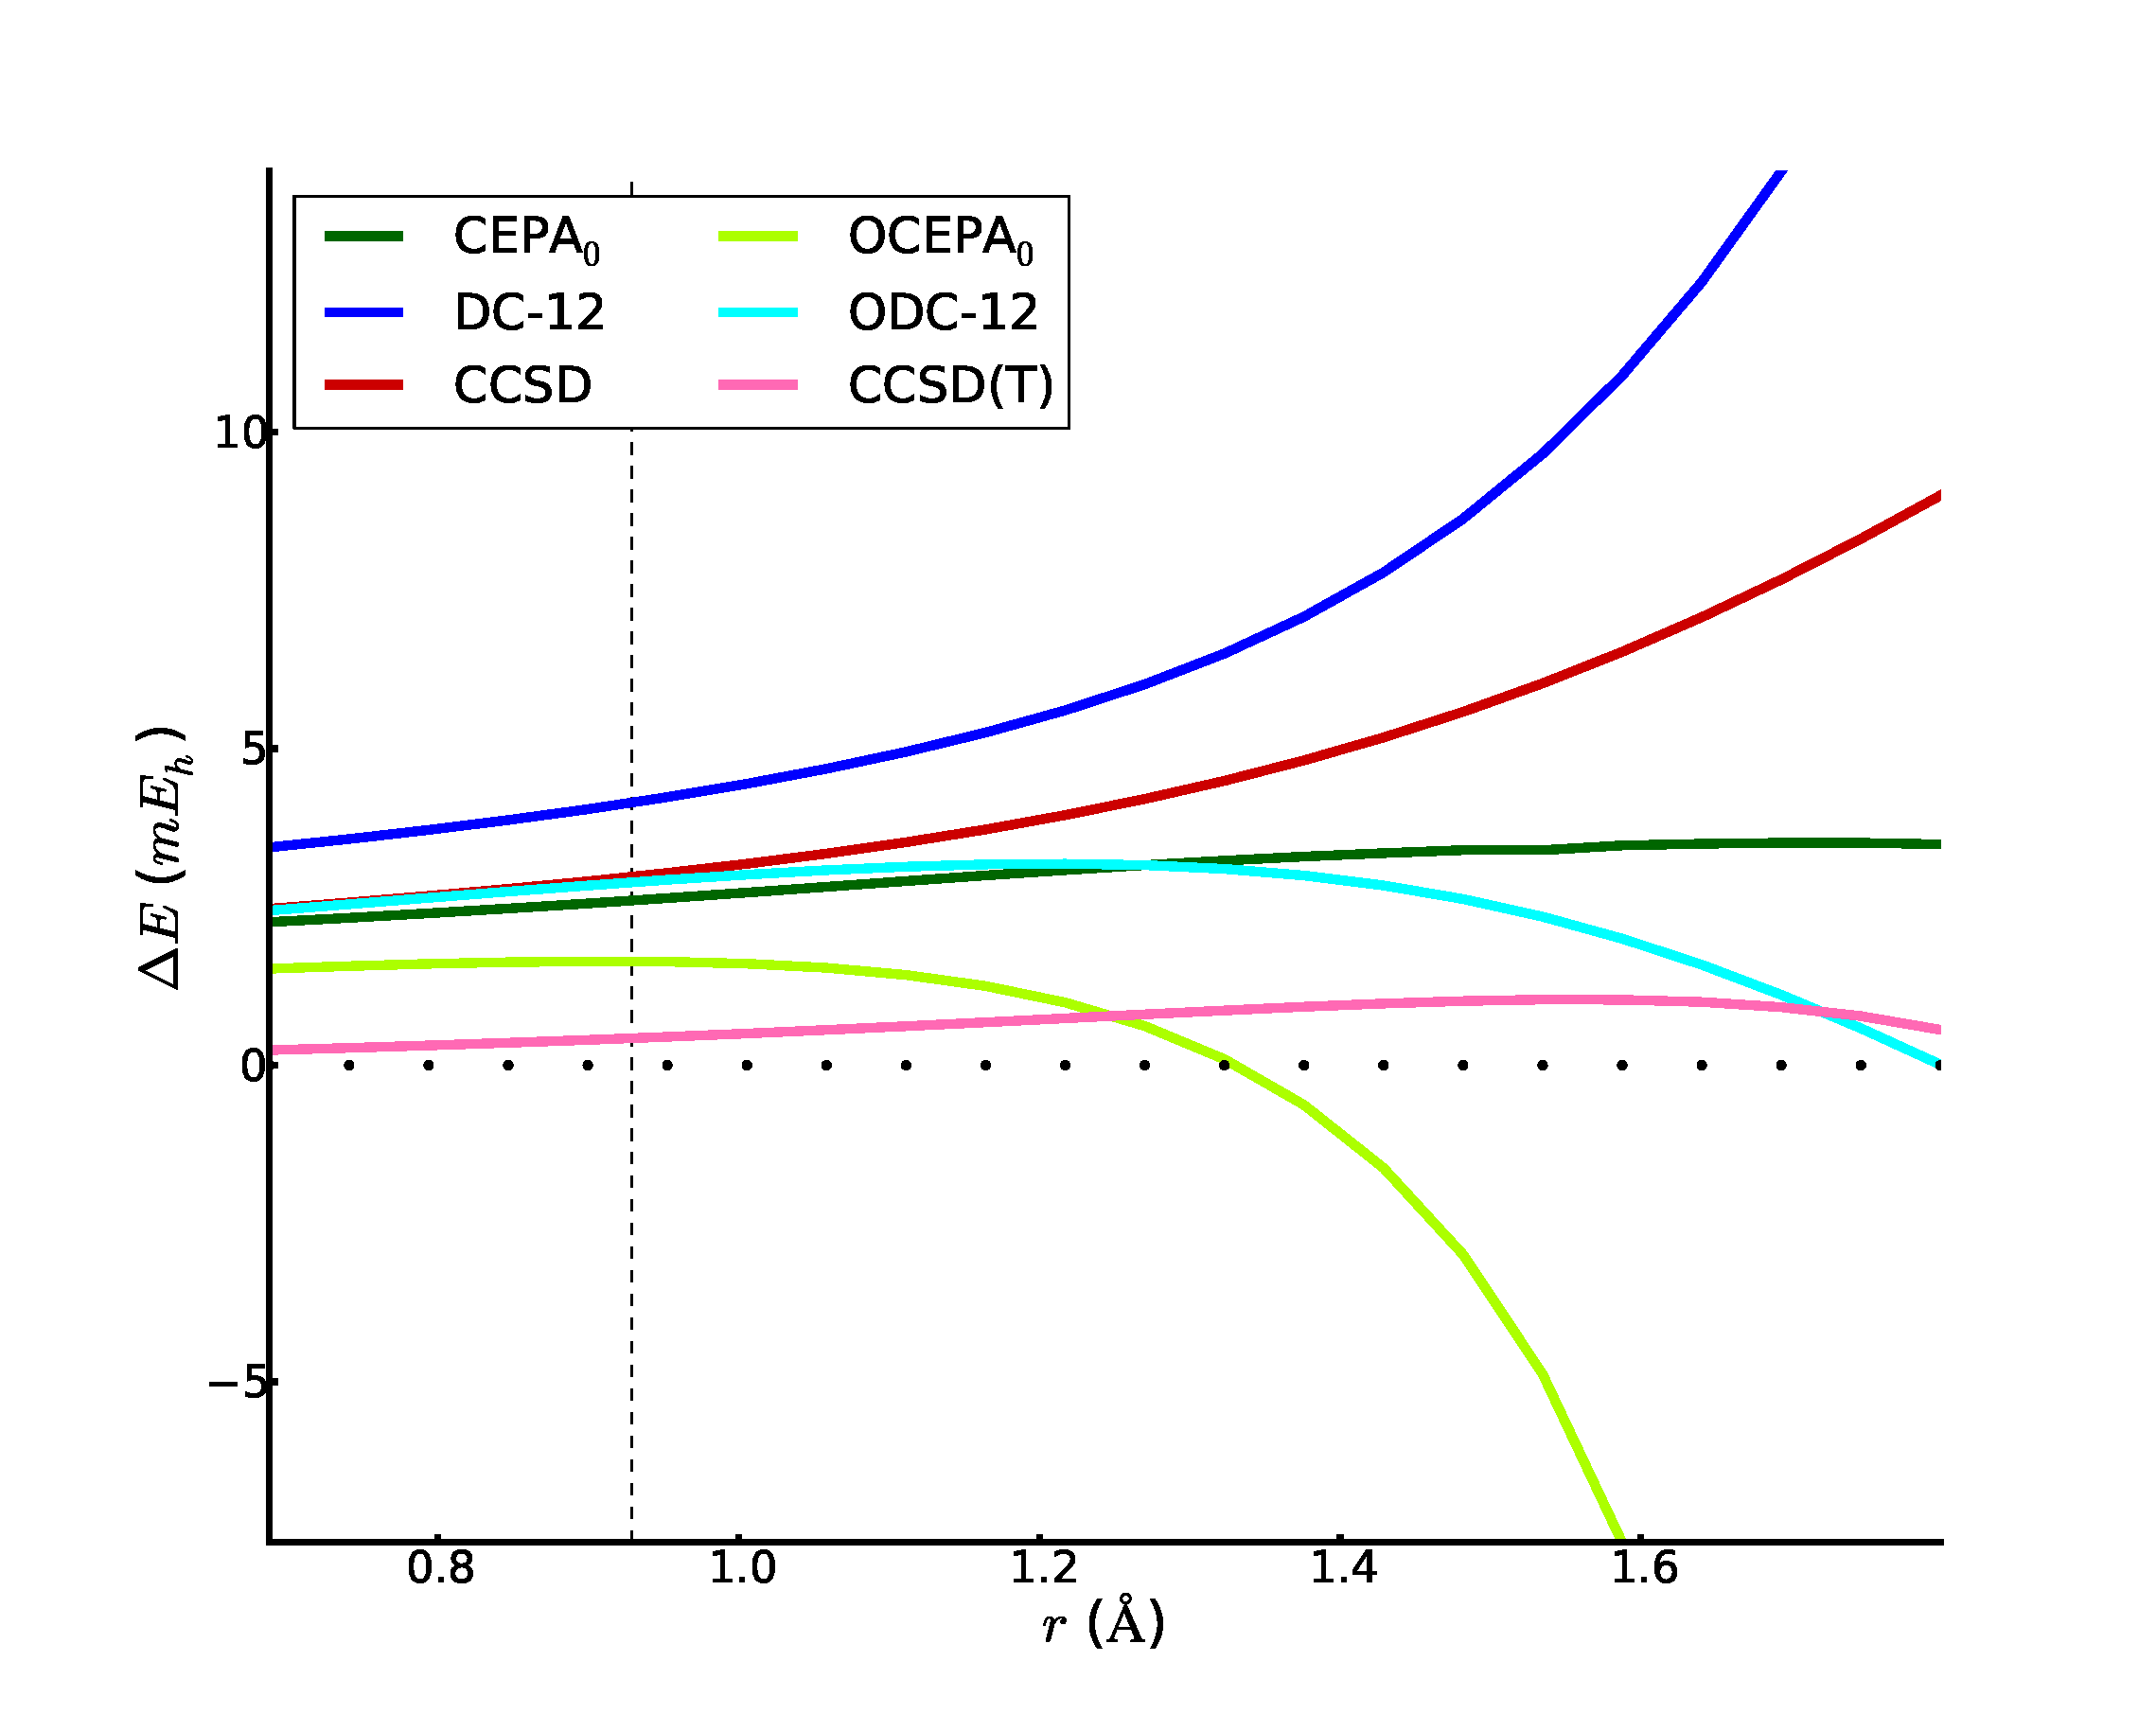
\includegraphics[width=0.8\textwidth]{figures/hf.pdf}
\end{figure}

\begin{figure}
	\centering
	\caption{%
        \label{beo-f}
        Error in the total energy (\mhartree), relative to full CI, as a
        function of Be--O internuclear separation (\AA) computed using six
        methods with the 6-31G basis set.
        The full CI reference is depicted with a horizontal dotted line.
        The dashed vertical line indicates the full CI equilibrium bond
        distance.
	}
	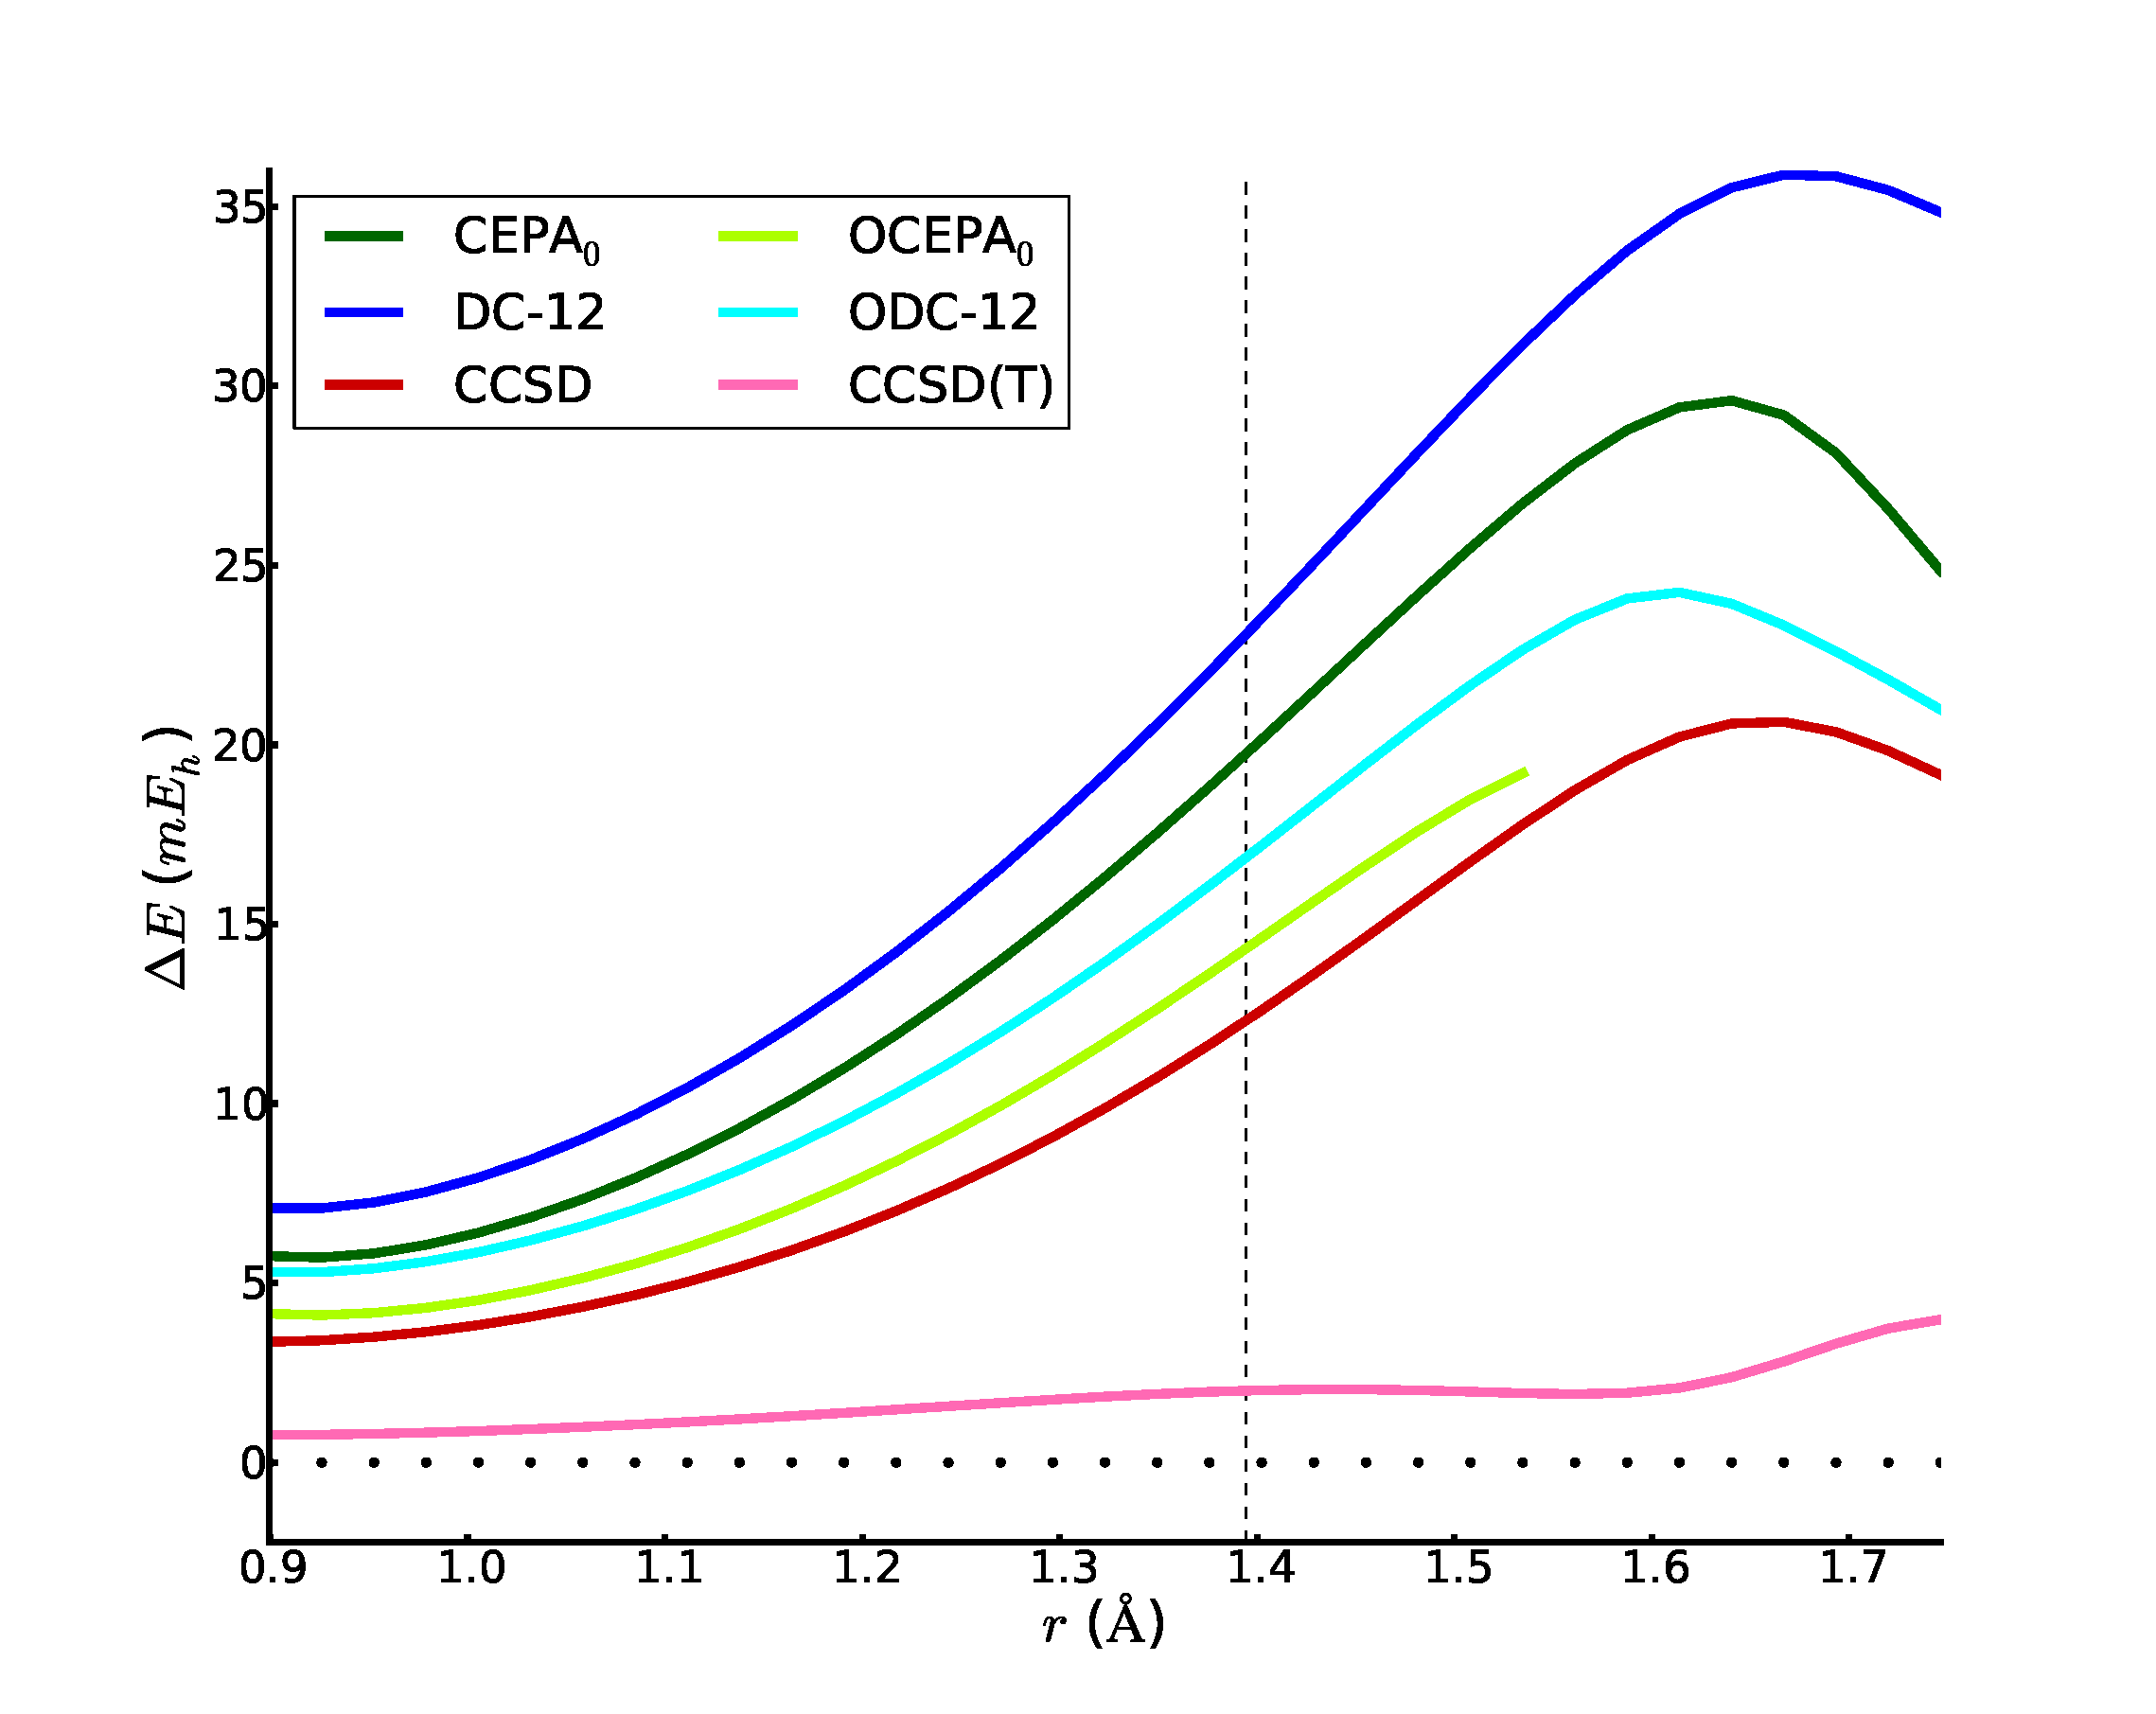
\includegraphics[width=0.8\textwidth]{figures/beo.pdf}
\end{figure}

\begin{figure}
	\centering
	\caption{%
        \label{n2-f}
        Error in the total energy (\mhartree), relative to full CI, as a
        function of N--N internuclear separation (\AA) computed using six
        methods with the 6-31G basis set.
        The full CI reference is depicted with a horizontal dotted line.
        The dashed vertical line indicates the full CI equilibrium bond
        distance.
	}
	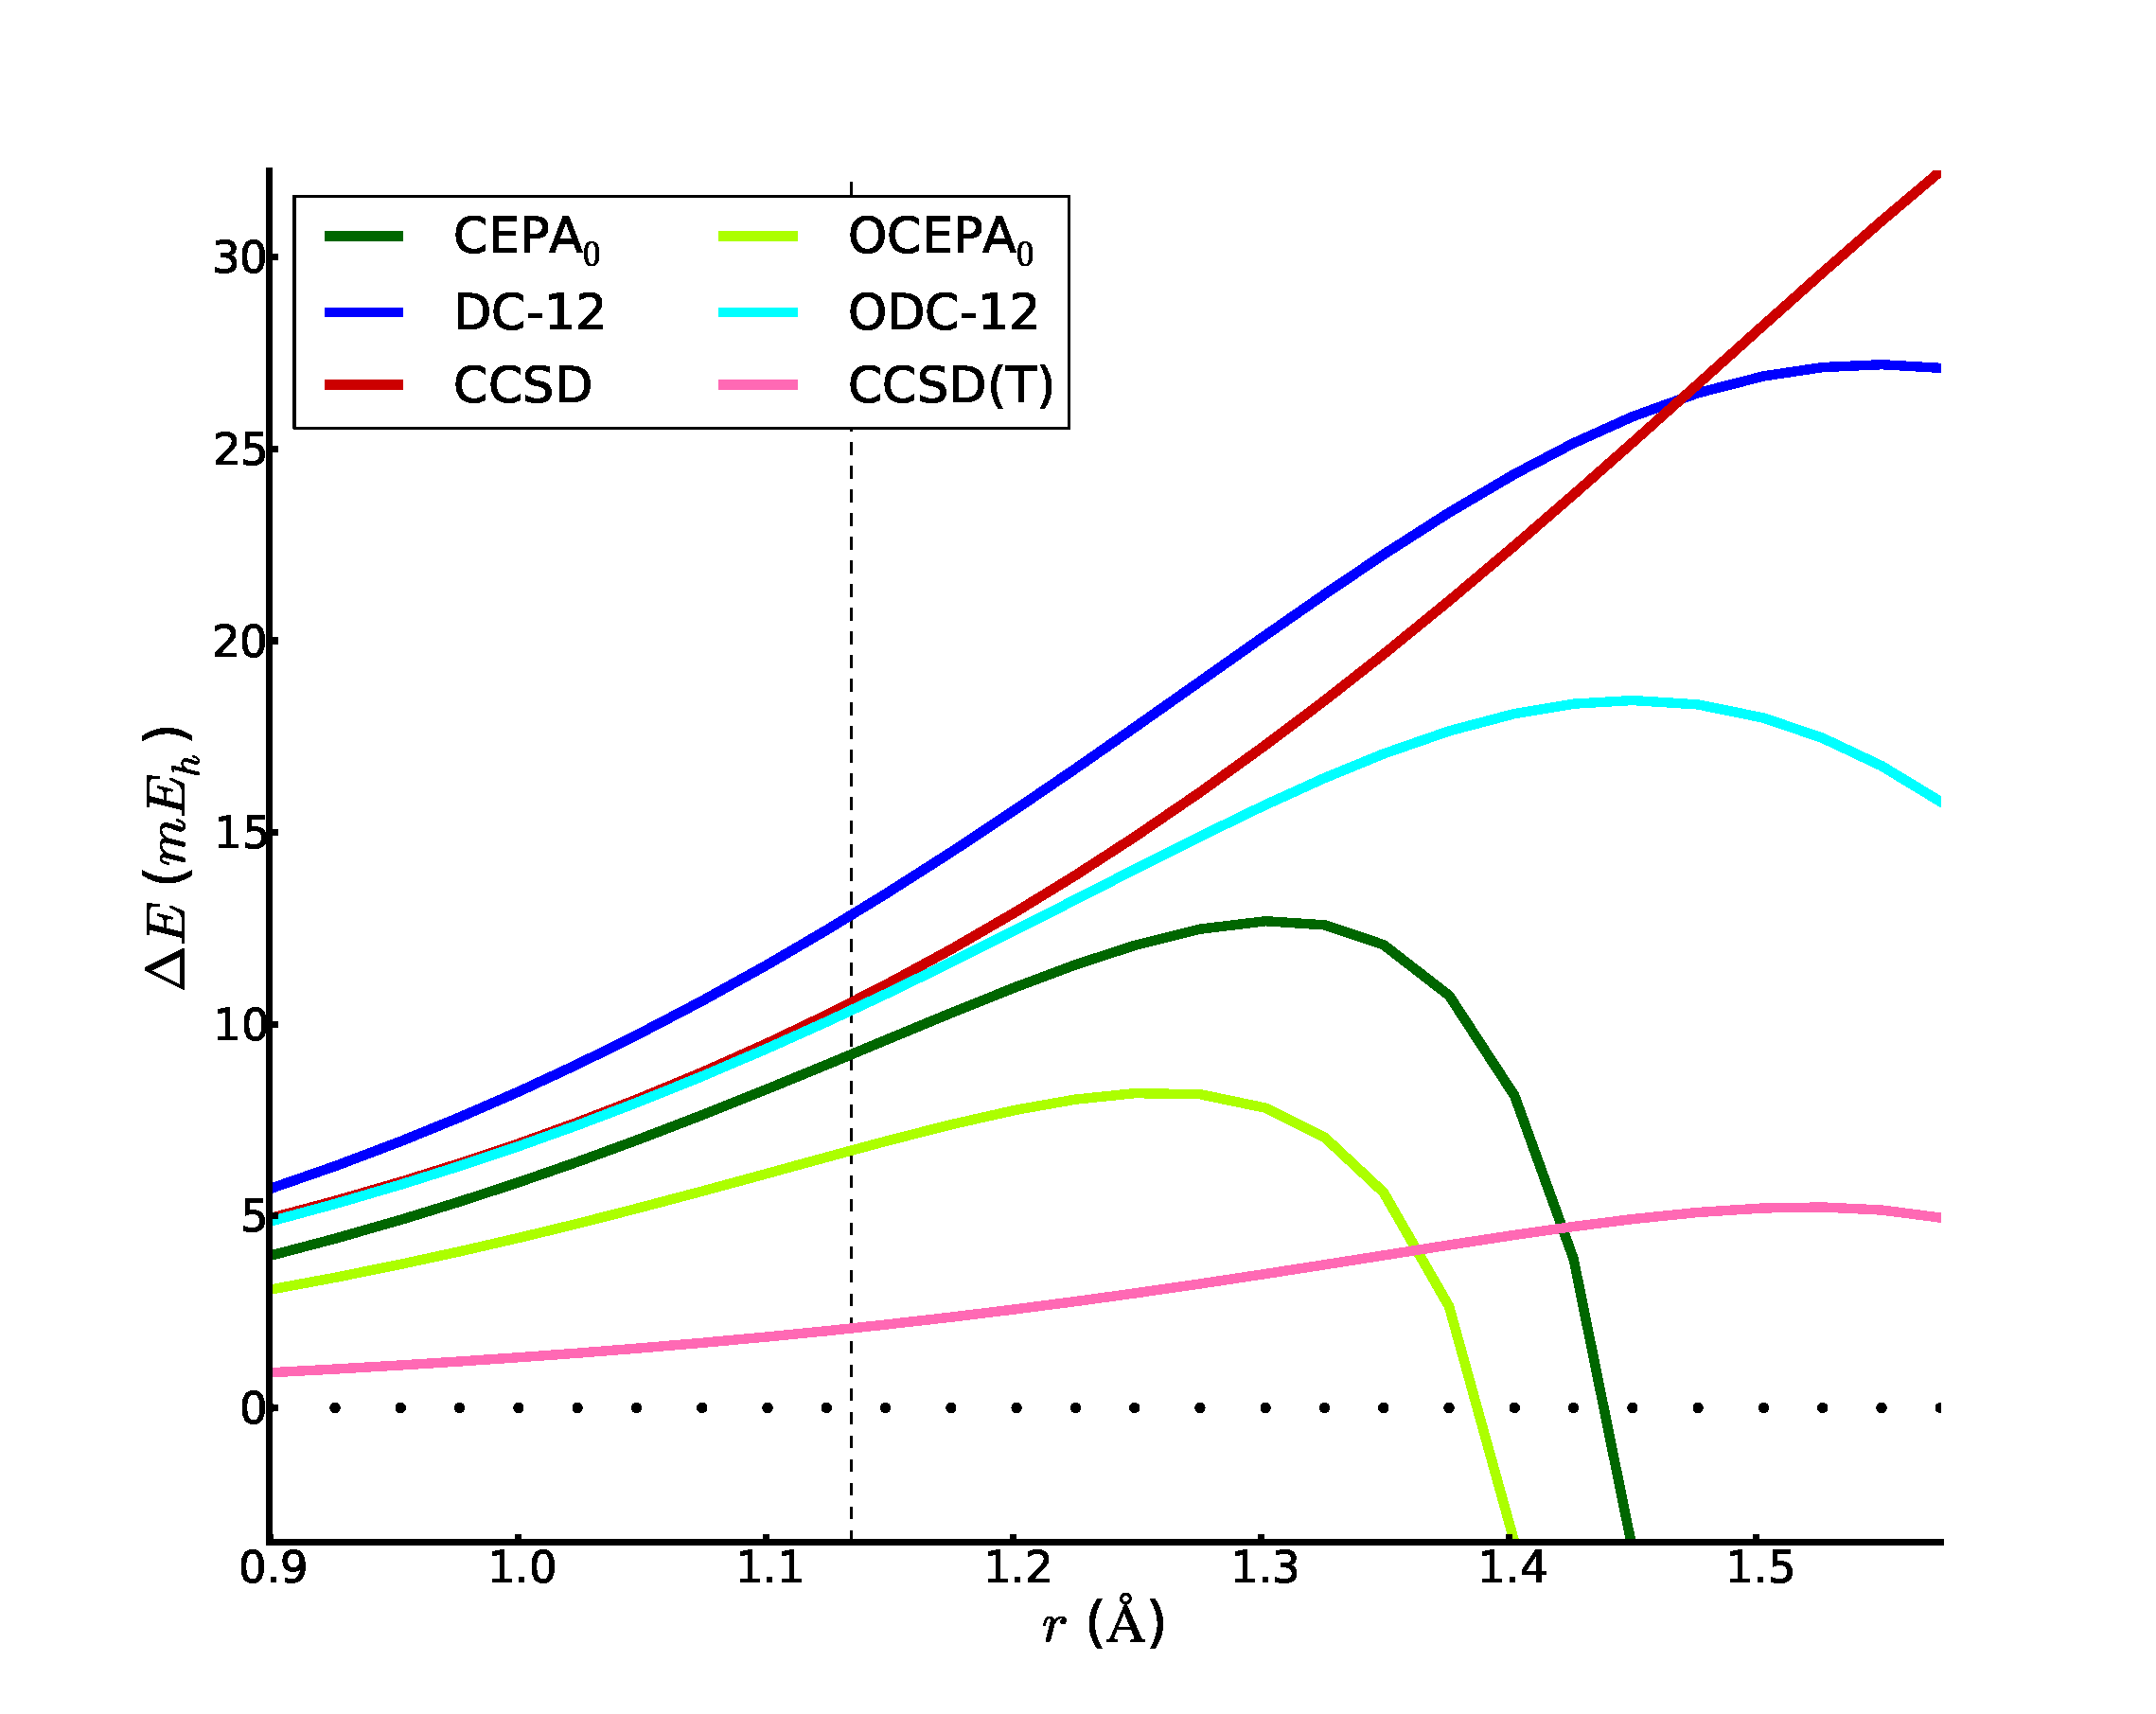
\includegraphics[width=0.8\textwidth]{figures/n2.pdf}
\end{figure}



\subsection{Covalent Bond Stretching in Diatomic Molecules}

Finally, we benchmark DCFT methods for covalent bond stretching.
Although accurate description of bond stretching demands the use of
multireference methods, our aim here is to explore the limits of DCFT away from
equilibrium.
For this purpose, we compute the energy as a function of bond distance for
diatomic molecules with single (HF and BH), double (BeO), and triple (\ce{N2})
bonds using the CEPA$_0$, OCEPA$_0$, DC-12, ODC-12, CCSD, and CCSD(T) methods.
We restrict ourselves to modest basis sets in order to use full CI (FCI) as a
reference, and plot the errors with respect to FCI ($\Delta E$) as a function of
internuclear distance for each molecule.
The relative performance of the methods is described below using non-parallelity
errors (NPE $=\Delta E_\mathrm{max}-\Delta E_\mathrm{min}$, \mhartree) computed
for specific bond distance ranges.


\paragraph{BH}

\Cref{bh-f} shows errors relative to FCI for the BH molecule.
DC-12 and CCSD increasingly overestimate the energy at larger internuclear
distances, whereas the CEPA$_0$ error curve is concave down.
Orbital optimization lowers the binding energy for OCEPA$_0$ even further
compared to CEPA$_0$, leading to large errors with respect to FCI for $r$(B--H)
> 1.5 \re, where \re is the FCI equilibrium bond distance (\re$=1.244$~\AA). At
1.87 \re, OCEPA$_0$ encounters convergence problems, which originate from
numerical instabilities due to the method's deficiencies in the description of
$N$-representability.
The ODC-12 method exhibits much more stable behavior with respect to bond
stretching in this case, fortuitously showing smaller errors and better
parallelity than CCSD(T).
For the range $[0.72\ \re, 2.47\ \re]$, the NPEs decrease in the order 
DC-12    (24~\mhartree) $>$
CEPA$_0$ (15) $>$
CCSD     (5) $>$
CCSD(T)  (3) $>$
ODC-12   (1).


\paragraph{HF}
Errors for HF bond stretching are plotted in \cref{hf-f}.
The $\Delta E$ values of CCSD and DC-12 increase as a function of $r$(H--F),
while CEPA$_0$ fortuitously maintains parallelity similar to CCSD(T) over the
range $[0.74\ \re, 1.94\ \re]$ ($\re = 0.929$~\AA).
OCEPA$_0$ increasingly overestimates the HF binding energy away from
equilibrium, failing to converge past 1.82 \re.
The ODC-12 method exhibits larger NPE than was observed for BH, and encounters
convergence problems past 1.94 \re.
CCSD(T) shows the best overall performance, with errors between 0 and
1~\mhartree.
In the range $[0.74\ \re, 1.94\ \re]$ the computed NPE values are:
DC-12    (15~\mhartree) $>$
CCSD     (7) $>$
ODC-12   (3) $>$
CEPA$_0$ (1) $\approx$
CCSD(T)  (1).
Recently, the orbital-optimized variants of CCSD(T) have been shown to yield
good performance for HF bond stretching.\cite{Bozkaya:2012p204114}

\paragraph{BeO}
The double bond of BeO presents a more challenging test for the single-reference
methods under consideration (\cref{beo-f}).
All methods but CCSD(T) show qualitatively similar error curves, with inflection
points near the FCI equilibrium ($\re=1.394$~\AA) and valleys/peaks around 0.6
\re/1.2 \re.
OCEPA$_0$ encounters convergence problems past 1.10 \re.
The ODC-12 method performs similarly to CCSD\@.
Overall, the NPEs for the range $[0.65\ \re, 1.10\ \re]$ decrease in the
following order:
DC-12    (29~\mhartree) $>$ 
CEPA$_0$ (24) $>$
ODC-12   (19) $>$
CCSD     (17) $>$
CCSD(T)  (3).

\paragraph{\ce{N2}}
\Cref{n2-f} depicts the errors relative to FCI for triple bond stretching in
\ce{N2}.
Here, OCEPA$_0$ fails to converge past 1.24 \re ($\re = 1.135$~\AA).
The ODC-12 method significantly overestimates the binding energy, possibly due
to the lack of three-body correlation effects, but shows much more stable
performance compared to methods other than CCSD(T).
NPEs in the range $[0.79\ \re, 1.39\ \re]$ decrease in the order:
CEPA$_0$ (802~\mhartree)\footnotemark $>$
\footnotetext{%
    CEPA$_0$ exhibits a vertical asymptote at 1.36 \re for N$_2$ stretching.
}
CCSD     (27) $>$
DC-12    (21) $>$
ODC-12   (14) $>$
CCSD(T)  (4).


\section{Conclusions}

We have presented the benchmark study of four density cumulant functional theory
(DCFT) methods (DC-06, DC-12, ODC-06, and ODC-12) developed recently in our
group.\cite{Simmonett:2010p174122,Sokolov:2012p054105,Sokolov:2013p024107,Sokolov:2013p204110}
Specifically we have compared the performance of DCFT to that of coupled
electron pair methods (CEPA$_0$ and OCEPA$_0$), as well as coupled-cluster
theory [CCSD and CCSD(T)] for predicting a variety of chemical properties
relevant to thermochemistry and kinetics, with a particular focus on open-shell,
electron-dense, and non-equilibrium systems.

Our results indicate that among the four DCFT methods, the best agreement with
available reference data is obtained for the ODC-12 method.
While all four DCFT formulations yield similar results for the description of
noncovalent interactions, DC-06, DC-12, and ODC-06 exhibit worse performance
than ODC-12 for thermodynamic and kinetic properties of reactions involving
open-shell molecules.
In particular, DC-06 and ODC-06 frequently encounter convergence problems that
originate from poor description of $N$-representability.
In comparing ODC-12 to other methods, several trends can be observed: 

(i) For all benchmark datasets, ODC-12 outperforms CCSD with errors smaller by
almost a factor of two, on average.
ODC-12 is also superior to CCSD for the description of single bond stretching in
BH and HF, although it does not converge for all bond distances.

(ii) The performance of ODC-12 and OCEPA$_0$ is comparable.
In particular, for hydrogen-transfer reaction barrier heights, the OCEPA$_0$
method yields smaller percent errors than ODC-12, whereas, for the radical
stabilization energies (RSE) and adiabatic ionization energies (AIE) in
electron-dense molecules, the ODC-12 method smaller standard deviations than
OCEPA$_0$.
For AIEs, ODC-12 gives smaller mean absolute deviations by almost a factor of
two.
ODC-12 also shows significantly smaller non-parallelity errors than OCEPA$_0$
for covalent bond stretching, and can be converged for a larger range of
distances for all diatomic molecules studied.

(iii) For the two most challenging datasets, RSE and AIE, the standard deviation
of ODC-12 and CCSD(T) are similar.
While CCSD(T) yields smaller mean absolute errors for the RSE database, the
ODC-12 method significantly outperforms CCSD(T) for the AIE test case.
However, for bond stretching ODC-12 is competitive with CCSD(T) only for the BH
dissociation and shows worse results for other molecules.

Overall, the data presented herein indicates that the ODC-12 method can be used
as an efficient $\mathcal{O}(n^6)$ alternative to CCSD, capable of predicting
thermodynamic and kinetic quantities that are competitive in accuracy with the
``gold-standard'' $\mathcal{O}(n^7)$ CCSD(T).
Although our current implementation of ODC-12 is far from optimal, the ODC-12
equations have reduced non-linearities compared to CCSD, which makes them more
amenable to parallel implementation.
The efficiency of ODC-12 can also greatly benefit from
spin-adaptation,\cite{Kutzelnigg:1999p2800,Kutzelnigg:2002p4787,Kutzelnigg:2010p433}
local
approximations,\cite{Werner:2003p8149,Taube:2005p837,Neese:2009p064103,Neese:2009p114108}
and density
fitting.\cite{Vahtras:1993p514,Hetzer:2000p9443,Schutz:2001p661,Werner:2003p8149}
Another important advantage of ODC-12 over CCSD is its stationarity, which makes
the computation of first-order properties and analytic gradients more efficient
and easily accessible.
In particular, ODC-12 has potential to be used for computing accurate response
properties which do not suffer from a lack of
gauge-invariance.\cite{Pedersen:1999p8318,Pedersen:2001p6983}

\chapter[%
    Linear-Response Density Cumulant Theory for Excited States:\\
	First Implementation and Benchmark Calculations
]{%
    Linear-Response Density Cumulant Theory for Excited States:\\
	First Implementation and Benchmark Calculations\footnote{%
        A.~V.~Copan and A.~Yu.~Sokolov (to be submitted in
        J.~Chem.~Theory~Comput).
    }
}
\label{ch:response}


\section{Abstract}

We present a linear-response formulation of density cumulant functional theory
(DCT) that provides accurate access to many electronic states.
DCT expresses the electronic energy as a Hermitian, size-extensive, and
stationary functional of the one-particle density matrix and the two-particle
density cumulant.
In the original DCT formulation only the information about a single electronic
state (usually, the ground state) is obtained.
In this research, we combine DCT with linear response theory to obtain
information about many electronic states simultaneously.
We discuss the derivation of linear-response DCT, present its implementation for
the ODC-12 method (LR-ODC-12), and benchmark its performance against highly
accurate equation-of-motion coupled cluster theory with up to full triple
excitations (EOM-CCSDT).
Our results for a set of small molecules demonstrate that LR-ODC-12 vertical
excitation energies are in closer agreement with EOM-CCSDT than those obtained
from equation-of-motion coupled cluster theory with up to double excitations
(EOM-CCSD).
In addition, we report a linear-response formulation of the orbital-optimized
linearized coupled cluster theory with double excitations (LR-OLCCD), which we
obtain by neglecting the non-linear terms in the LR-ODC-12 equations.


\section{Introduction}

Accurate simulation of excited electronic states remains one of the major
challenges in modern electronic structure theory. 
{\it Ab initio}\/ methods for excited states can be divided into
single-reference and multi-reference categories, based on their ability to
treat static electron correlation.
Multi-reference methods can correctly describe static correlation in
near-degenerate valence orbitals and electronic states with multiple-excitation
character, but often lack accurate treatment of important dynamic correlation
effects (e.g., multi-configurational self-consistent field or multi-reference
perturbation theories)
\cite{Knowles:1985p259,Werner:1985p5053,Wolinski:1987p225,Hirao:1992p374,Finley:1998p299,Andersson:1990p5483,Andersson:1992p1218,Werner:1996p645,Angeli:2001p10252,Angeli:2001p297}
or become very costly when the number of near-degenerate orbitals is large
(e.g., multi-reference configuration interaction or coupled cluster theories).
\cite{Mukherjee:1977p955,Lindgren:1978p33,Siegbahn:1980p1647,Jeziorski:1981p1668,Werner:1988p5803,Mahapatra:1998p157,Mahapatra:1999p6171,Pittner:2003p10876,Evangelista:2007p024102,Datta:2011p214116,Evangelista:2011p114102,Kohn:2013p176,Nooijen:2014p081102}
Meanwhile,
single-reference methods
\cite{Foresman:1992p135,Sherrill:1999p143,Geertsen:1989p57,Comeau:1993p414,Stanton:1993p7029,Krylov:2008p433,Crawford:2000p33,Shavitt:2009,Sekino:1984p255,Koch:1990p3345,Koch:1990p3333,Nooijen:1997p6441,Nooijen:1997p6812,Nakatsuji:1978p2053,Nakatsuji:1979p329}
often provide a compromise between the computational
cost and accuracy, and can be used to reliably compute properties of molecules
in low-lying electronic states near the equilibrium geometries. In these
situations, single-reference equation-of-motion coupled cluster theory
(EOM-CC)
\cite{Geertsen:1989p57,Comeau:1993p414,Stanton:1993p7029,Krylov:2008p433,Crawford:2000p33,Shavitt:2009}
is usually the method of choice, especially when high accuracy
is desired. 

The EOM-CC methods yield size-intensive excitation energies
\cite{Koch:1990p3345,Koch:1990p3333}
and can be
systematically improved by increasing the excitation rank of the cluster
operator in the exponential parametrization of the wavefunction. Although EOM-CC
is usually formulated in the context of a similarity-transformed Hamiltonian,
its excitation energies are equivalent to those obtained from linear-response
coupled cluster theory (LR-CC).
\cite{Sekino:1984p255,Koch:1990p3345,Koch:1990p3333}
Both EOM-CC and LR-CC are based on non-Hermitian eigenvalue problems,
complicating the computation of molecular properties (e.g., transition dipoles)
by requiring evaluation of left and right eigenvectors.
\cite{Stanton:1993p8840,Stanton:1994p4695,Stanton:1994p8938,Levchenko:2005p224106}
% may result in an incorrect description of potential energy surfaces in the
% vicinity of conical intersections where complex excitation energies may be
% obtained.  \cite{Hattig:2005p37,Kohn:2007p044105,Kjonstad:2017p164105}
Several Hermitian alternatives to EOM-CC and LR-CC have been
proposed to avoid these problems, such as  
algebraic diagrammatic construction
\cite{Schirmer:1982p2395,Schirmer:1991p4647,Schirmer:2004p11449,Harbach:2014p064113,Dreuw:2014p82}, 
unitary and variational LR-CC,
\cite{Taube:2006p3393,Kats:2011p062503,Walz:2012p052519}
similarity-constrained CC,
\cite{Kjonstad:2017p4801}
and propagator-based LR-CC.
\cite{Moszynski:2005p1109,Korona:2010p14977}

In this work, we present the development of linear-response density cumulant
functional theory (LR-DCT), a size-intensive approach for excited
electronic states. In density cumulant functional theory (DCT),
\cite{Kutzelnigg:2006p171101,Simmonett:2010p174122,Sokolov:2012p054105,Sokolov:2013p024107,Sokolov:2013p204110,Sokolov:2014p074111,Wang:2016p4833}
the
electronic energy is obtained by optimizing the energy functional directly in
terms of the one-particle reduced density matrix and the two-particle density
cumulant, a fully connected part of the two-particle reduced density matrix
(2-RDM).
\cite{Fulde:1991,Ziesche:1992p597,Kutzelnigg:1997p432,Mazziotti:1998p419,Mazziotti:1998p4219,Kutzelnigg:1999p2800,Ziesche:2000p33,Herbert:2007p261,Kong:2011p214109,Hanauer:2012p50}
In this regard, DCT is related to approaches that are based on
the variational optimization
\cite{Colmenero:1993p979,Nakatsuji:1996p1039,Mazziotti:1998p4219,Mazziotti:2006p143002,Kollmar:2006p084108,DePrince:2007p042501,DePrince:2016p164109}
or parametrization
\cite{Mazziotti:2008p253002,Mazziotti:2010p062515,DePrince:2012p1917}
of 2-RDM\@. On
the other hand, DCT has a close relationship
\cite{Sokolov:2013p024107,Sokolov:2013p204110}
with wavefunction-based electronic
structure theories, such as linearized, unitary, and variational coupled
cluster theory.
\cite{Kutzelnigg:1991p349,Kutzelnigg:1998p65,VanVoorhis:2000p8873,Kutzelnigg:1982p3081,Bartlett:1989p133,Watts:1989p359,Szalay:1995p281,Cooper:2010p234102,Evangelista:2011p224102}
In contrast to variational 2-RDM theory
\cite{Nakata:2009p042109,vanAggelen:2010p114112,Verstichel:2010p114113}
and traditional
coupled cluster methods [e.g., CCSD and CCSD(T)],
\cite{Crawford:2000p33,Shavitt:2009}
DCT naturally combines
size-extensivity and a Hermitian energy functional. In addition, the DCT
electronic energy is fully relaxed with respect to all of its parameters, which
greatly simplifies computation of the first-order molecular properties.
\cite{Scheiner:1987p5361,Salter:1989p1752,Gauss:1991p2623,Gauss:1991p207}
We have successfully applied DCT to a variety of chemical systems with
different electronic structure effects (e.g., open-shell, symmetry-breaking,
and multi-reference).
\cite{Sokolov:2013p204110,Sokolov:2014p074111,Wang:2016p4833,Copan:2014p2389,Mullinax:2015p2487}
One limitation of the original DCT formulation is
that it can only obtain information about the lowest-energy state of a
particular symmetry (usually, the ground state). By combining DCT with linear
response theory, we remove this limitation, providing access to many electronic
states simultaneously.

We begin with a brief overview of DCT (\cref{sec:dct}) and linear response
theory (\cref{sec:lr}). We then discuss the derivation of linear-response
theory for the ODC-12 method (LR-ODC-12, \cref{sec:lr_odc12}).
% and the details of its implementation (\cref{sec:implementation}). 
In section \cref{sec:olccd}, 
we derive equations for the linear-response orbital-optimized linearized
coupled cluster theory with double excitations (LR-OLCCD), which we obtain by
neglecting the non-linear terms in the LR-ODC-12 equations. 
We outline the
computational details in \cref{sec:comp_details}.
In section \cref{sec:results}, we demonstrate that the LR-ODC-12 excitation
energies are size-intensive (\cref{sec:size_intensivity}), test the performance
of LR-ODC-12 for the dissociation of \ce{H2} (\cref{sec:two_electron}), and
benchmark the accuracy of LR-ODC-12 for vertical
excitation energies of small molecules (\cref{sec:vert_excit}).
Finally, we present our conclusions in section \cref{sec:conclusions}. 

\chapter[%
    Algorithms for Linear-Response Density Cumulant Theory
]{%
    Algorithms for Linear-Response Density Cumulant Theory
}
\label{ch:davidson}

\cref{ch:response} presented the LR-ODC-12 model for electronic excited states,
where excitation energies and transition properties are computed by
diagonalizing the parameter Hessian of the ODC-12 energy functional, with
respect to a metric that arises from the time-dependence of the parameter
responses.
Since number of parameters in the ODC-12 model scales as
\(
    \mathcal{O}(o^2v^2)
\)
with the number of occupied (\(o\)) and virtual (\(v\)) orbitals, the
memory requirement for the Hessian matrix scales with the fourth power
of \(o\) and \(v\), and the number of floating point operations needed
to diagonalize it scales with the sixth power of these dimensions.
Such a brute-force approach will rapidly overwhelm available computing
resources even for relatively small molecules.
For the common scenario in which we only care about states within a narrow
energy range, the cost of diagonalization can be drastically reduced through the
use of so-called {\itshape direct algorithms} which enable the determination of
subsets of eigenvectors and eigenvalues without explicitly constructing the
Hessian matrix in computer memory.
This chapter will explore the use of the Davidson
algorithm\cite{Liu:1978p49,Davidson:1975p87} in solving the LR-ODC-12 model.
\cref{sec:davidson:davidson} describes the Davidson algorithm in general terms
and describes strategies employed in the present implementation to reduce memory
usage for large calculations.
\cref{sec:davidson:eig} discusses the structure of the LR-ODC-12 eigenvalue
equations, which is followed by a comparison of several alternative strategies
for solving the LR-ODC-12 model in section \cref{sec:davidson:strategies}.


\section{The Davidson Algorithm}
\label{sec:davidson:davidson}

Direct algorithms represent linear transformations as functions mapping vectors
\(
    \mathbf{v}
\)
in their domain to vectors
\(
    \mathbf{L}(\mathbf{v})
\)
in their codomain, rather than as coefficient arrays
\(
    [L_{ij}]
    =
    [\mathbf{e}_i \cdot \mathbf{L}(\mathbf{e}_j)]
\)
over a complete basis.
That is, the result of the transformation is determined {\itshape directly},
without explicitly forming its matrix representation in computer memory.
The Davidson algorithm applies this technique in the context of a matrix
diagonalization, by progressively growing a basis
\(
    \{\mathbf{u}_1, \ldots,\mathbf{u}_d\}
\)
to span the lowest or highest eigenvectors of a matrix to some threshold of
accuracy.
For a transformation on \(\mathbb{R}^n\), this allows us to reduce our
computational effort from \(\mathcal{O}(n^3)\) to \(\mathcal{O}(n^2 d)\) or even
less when \(\mathbf{L}\) is constructed from lower-dimensional arrays.
Memory requirements are reduced from \(\mathcal{O}(n^2)\) to \(\mathcal{O}(nd)\)
in the Davidson algorithm, so that, as long as the dimension of the
transformation is large relative to the desired number of roots, we can gain
considerable savings.

\begin{algorithm}
    \caption{%
        Canonical multiroot Davidson algorithm for a generic eigenvalue problem,
        $\mathbf{L}\mathbf{v}_j=\lambda_j\mathbf{G}\mathbf{v}_j$, with periodic
        subspace collapse.
        Requires linear transformation functions and diagonal approximations
        (indicated by tildes) for \(\mathbf{L}\) and \(\mathbf{G}\)
        and solves for the lowest \(k\) eigenvalues and eigenvectors.
    }
    \label{algo:davidson}
    \begin{algorithmic}[1]
        \Procedure{Davidson}{%
            $
            \mathbf{L}(\cdot),
            \mathbf{G}(\cdot),
            \tilde{\mathbf{L}},
            \tilde{\mathbf{G}},
            \mathbf{U}^{(0)},
            k,
            d_\mathrm{max},
            i_\mathrm{max},
            r_\mathrm{tol}
            $%
        }
        \State
        Initialize the expansion space with a set of guess vectors,
        \(\mathbf{U}\leftarrow\mathbf{U}^{(0)}\).
        \For{$1\leq i\leq i_\mathrm{max}$}{}
            \State
            Construct subspace representation and solve the lowest \(k\)
            eigenvalues.
            \[
                \mathbf{L}^\mathrm{sub}
                =
                \mathbf{U}^\dagger
                \mathbf{L}(\mathbf{U})
            \]
            \[
                \mathbf{G}^\mathrm{sub}
                =
                \mathbf{U}^\dagger
                \mathbf{G}(\mathbf{U})
            \]
            \[
                \mathbf{L}^\mathrm{sub}
                \mathbf{v}_j^\mathrm{sub}
                =
                \lambda_j
                \mathbf{G}^\mathrm{sub}
                \mathbf{v}_j^\mathrm{sub}
            \]
            \State
            Calculate the eigenvector residuals over the full space.
            \[
                \mathbf{r}_j
                =
                (
                    \mathbf{L}(\mathbf{U})
                    -
                    \lambda_j
                    \mathbf{G}(\mathbf{U})
                )
                \mathbf{v}_j^\mathrm{sub}
            \]
            \If{$\max(\mathbf{r}_j) < r_\mathrm{tol}$ for all $j$}
                \State
                Set
                \(\mathbf{v}_j\leftarrow\mathbf{U}\mathbf{v}_j^\mathrm{sub}\)
                and quit the loop.  The eigenvectors are converged.
            \EndIf
            \State
            Determine new direction vectors by preconditioning the residual.
            \[
                \mathbf{d}_j^{(i)}
                =
                -
                (
                    \tilde{\mathbf{L}}
                    -
                    \lambda_j
                    \tilde{\mathbf{G}}
                )^{-1}
                \mathbf{r}_j
            \]
            \State
            Project out the span of \(\mathbf{U}\) and orthogonalize via
            SVD compression.
            \[
                \widehat{\mathbf{U}}^{(i)}
                =
                (\mathbf{1} - \mathbf{U}^\dagger \mathbf{U})
                \mathbf{D}^{(i)}
            \]
            \[
                \widehat{\mathbf{U}}^{(i)}
                \approx
                \mathbf{U}^{(i)}
                \mathbf{\Sigma}^{(i)}
                \mathbf{W}^{(i)\dagger}
            \]
            \If{%
                $
                \mathrm{rank}(\mathbf{U})
                +
                \mathrm{rank}(\mathbf{U}^{(i)})
                <
                d_\mathrm{max}
                $%
            }
                \State
                Extend the expansion space,
                \(
                    \mathbf{U}
                    \leftarrow
                    (\mathbf{U}\ \mathbf{U}^{(i)})
                \)
            \Else
                \State
                Collapse the expansion space,
                \(
                    \mathbf{U}
                    \leftarrow
                    (
                        \mathbf{U}
                        \mathbf{v}_1^\mathrm{sub}\ 
                        \cdots\ 
                        \mathbf{U}
                        \mathbf{v}_k^\mathrm{sub}
                    )
                \).
            \EndIf
        \EndFor
        \State
        {\bfseries return}
        \(
            \lambda_j,
            \mathbf{v}_j
        \)
        \EndProcedure
    \end{algorithmic}
\end{algorithm}

The procedure for the generalized Davidson algorithm is presented in
\cref{algo:davidson}, which solves for the eigenvalues and right eigenvectors of
a generalized eigenvalue problem, which may or may not be symmetric.
The strategy of the algorithm is as follows.
We expand our transformations in the reduced expansion space,
\(
    [L_{ij}^\mathrm{sub}]
    =
    [\mathbf{u}_i\cdot \mathbf{L}(\mathbf{u}_j)]
\),
and solve the eigenvalue equation in this subspace.
\begin{equation}
    \mathbf{L}^\mathrm{sub}
    \mathbf{v}_j^\mathrm{sub}
    =
    \lambda_j^\mathrm{trial}
    \mathbf{G}^\mathrm{sub}
    \mathbf{v}_j^\mathrm{sub}
\end{equation}
This trial solution is expressed in the full space as
\(
    \mathbf{v}_j^\mathrm{trial}
    =
    \mathbf{U}\mathbf{v}_j^\mathrm{sub}
\).
The correction vector
\(
    \mathbf{d}_j
    =
    \mathbf{v}_j^\mathrm{trial}
    -
    \mathbf{v}_j
\)
taking us to the exact solution can be approximated as
\begin{equation}
    \label{eq:davidson:davidson-step}
    \mathbf{d}_j
    \approx
    -
    (
        \tilde{\mathbf{L}}
        -
        \lambda_j^\mathrm{trial}
        \tilde{\mathbf{G}}
    )^{-1}
    \mathbf{r}_j
\end{equation}
where
\(
    \mathbf{r}_j
    \equiv
    (\mathbf{L} - \lambda_j^\mathrm{trial}\mathbf{G})
    \mathbf{v}_j^\mathrm{trial}
\)
is the residual vector and
\(
    (
        \tilde{\mathbf{L}} - \lambda^\mathrm{trial}\tilde{\mathbf{G}}
    )^{-1}
\)
is called the preconditioner, which is constructed from diagonal
approximations to \(\mathbf{L}\) and \(\mathbf{G}\).
This correction vector can be motivated as an approximate solution to the
following identity.
\begin{equation}
    \mathbf{0}
    =
    (\mathbf{L} - \lambda_j\mathbf{G})
    \mathbf{v}_j
    =
    (\mathbf{L} - \lambda_j\mathbf{G})
    (
        \mathbf{v}_j^\mathrm{trial}
        +
        \mathbf{d}_j
    )
\end{equation}
By repeatedly adding these correction vectors to the subspace, one can
iteratively grow the expansion space until it spans the desired eigenvector,
\(\mathbf{v}_j\).
At convergence, the residual and the correction vectors become vanishingly
small.
A key assumption of this algorithm is that the matrices are diagonally
dominant, otherwise the diagonal approximation in
\cref{eq:davidson:davidson-step} breaks down and the procedure will
fail to converge on the desired roots.
When the expansion space becomes large, we can periodically replace the
expansion vectors with the current set of trial eigenvectors in order to
keep the memory requirements more manageable.
For very large matrices, frequent collapses every second or third iteration can be used to keep I/O requirements to a minimum, at the cost
of slower convergence.\cite{Leininger:2001p1574}
This approach is quite general and can be adapted to other large matrix
problems, such as the linear equation
\(\mathbf{L}\mathbf{x}=\mathbf{b}\), where it yields a variant of the
conjugate gradient method.

\afterpage{%
    \clearpage
    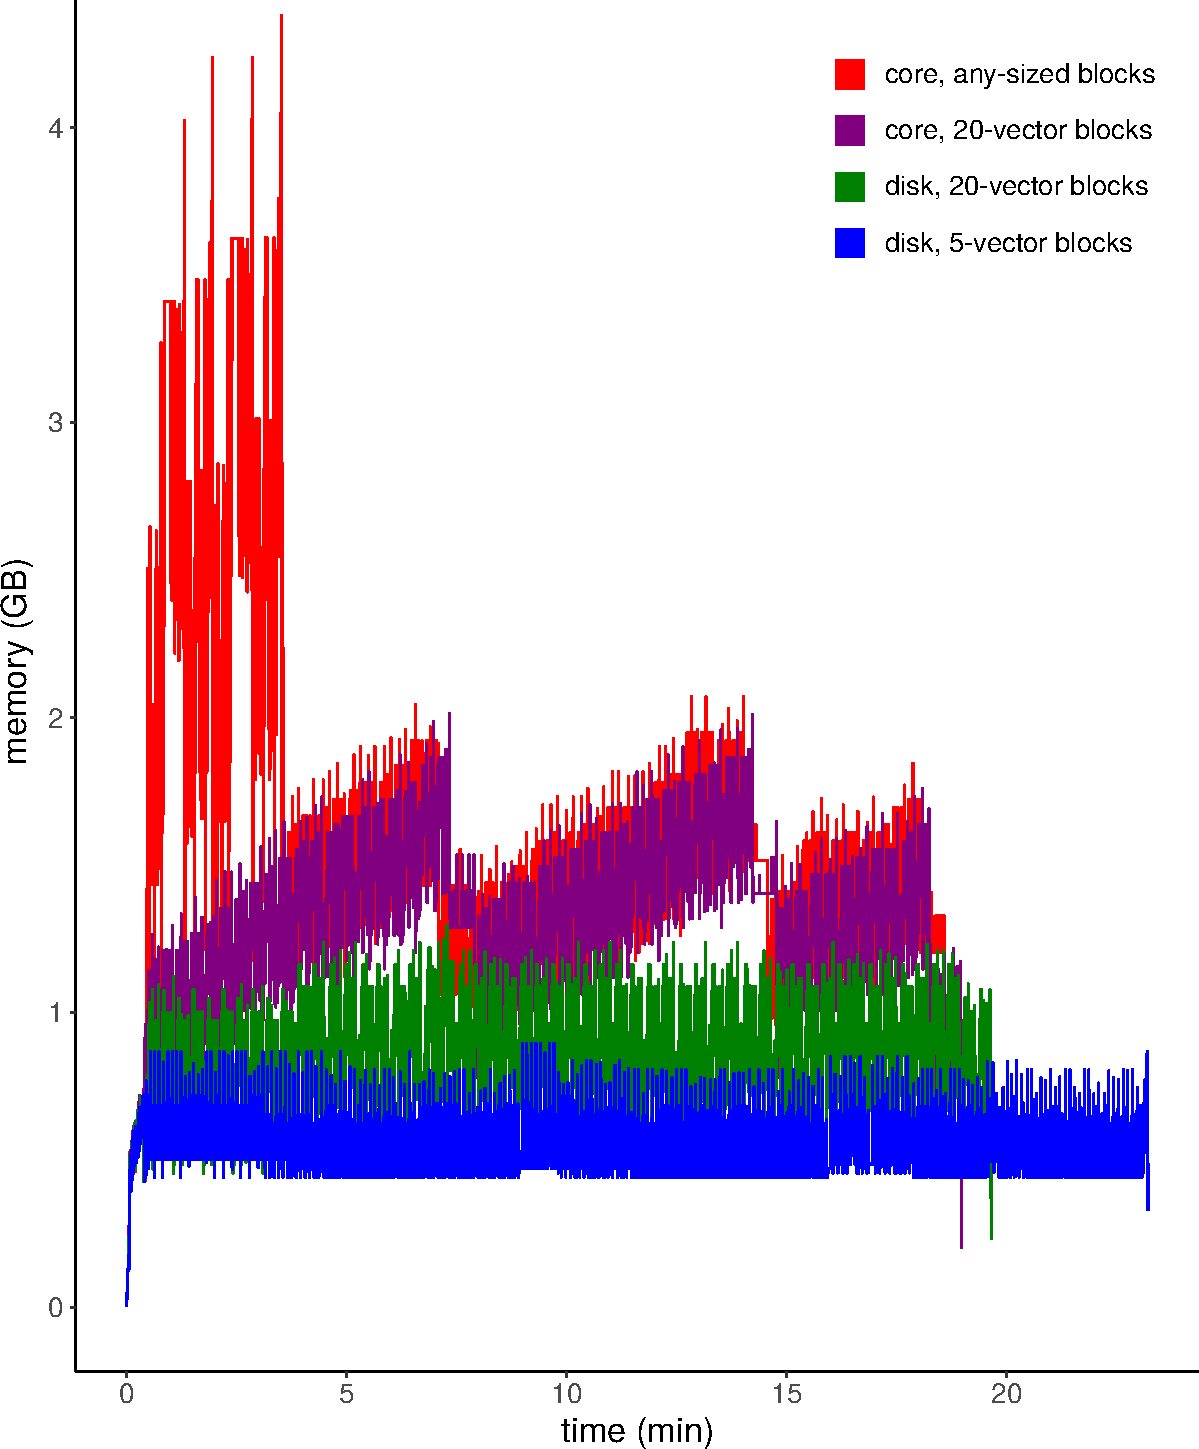
\includegraphics[width=0.9\textwidth]{figures/mem_edited.pdf}
    \captionof{figure}{%
        \label{fig:davidson:memory-profiles}
        Memory profiles for calculating the lowest 20 states of ethylene with
        the def2-SV(P) basis set on an Intel\textsuperscript{\textregistered}
        Core\texttrademark\ i7-5600U processor using
        \cref{eq:davidson:canonical-reduced,eq:davidson:fock-diagonal} below.
        Starts from a set of 100 guess vectors and periodically collapses the
        expansion space to keep the number of vectors under 200.
        The green and blue trace result from storing vectors and integral arrays
        on disk, whereas the red and purple ones use only RAM.
    }
}

\cref{fig:davidson:memory-profiles} presents memory profiles for the Davidson
algorithm, as implemented for the present study.
The red trace represents the most straight-forward implementation of
\cref{algo:davidson}.
Note that the images \(\mathbf{L}(\mathbf{u}_i)\) are only evaluated once as
these vectors are added to the expansion space and are reused on future
iterations.
The large spike in memory between 0 and 3 minutes in the runtime comes from the
initial evaluation of the transformation on the guess vectors.
This can be mitigated by breaking the expansion space into blocks of no more
than 20 vectors, so that the guess vector evaluations have the same cost as the
latter transformations.
The result is depicted as the purple trace, where we see that the early memory
spike has been smoothed at negligible cost to the runtime.
The sawtooth shape of the red and purple traces between 3 and 18 minutes
depicts the periodic collapse of the expansion space, which would otherwise
continue to build indefinitely as the algorithm proceeds.
Storing the Davidson vectors and the all-virtual integral arrays,
\(\overline{g}_{ab}^{cd}\) and \(\mathcal{G}_{ab}^{cd}\), on disk produces the
green trace, which irons out the sawtooth shape in the trajectory at the cost
of some additional runtime for retrieving arrays that are stored on disk.
Finally, the blue trace shows that the memory usage can be reduced below 1~GB by
shrinking the block sizes even further, albeit at the cost of some additional
I/O overhead.


\section{The LR-ODC-12 Eigenvalue Equation}
\label{sec:davidson:eig}

The LR-ODC-12 eigenvalue equation has a two-by-two block structure which
describes the independent variation of the parameters and their complex
conjugates.
\begin{equation}
    \label{eq:linear-response-eigenvalue-equation}
    \mathbf{E}\mathbf{z}_k
    =
    \omega_k
    \mathbf{M}\mathbf{z}_k
    ,
    \quad
    \mathbf{E}
    =
    \begin{pmatrix}
        \mathbf{A} & \mathbf{B} \\
        \mathbf{B}^* & \mathbf{A}^*
    \end{pmatrix}
    ,
    \quad
    \mathbf{M}
    =
    \begin{pmatrix}
        \mathbf{S} & \mathbf{0} \\
        \mathbf{0} & -\mathbf{S}^*
    \end{pmatrix}
    ,
    \quad
    \mathbf{z}_k
    =
    \begin{pmatrix}
        \mathbf{x}_k \\
        \mathbf{y}_k
    \end{pmatrix}
\end{equation}
This block symmetry leads to a paired system of eigenvalues,
\(
    \{\pm\omega_k\}
\).
The submatrices in \cref{eq:linear-response-eigenvalue-equation} are further
blocked according to whether they describe variations of the one-body
(\(\mathbf{t}_1\)) or two-body (\(\mathbf{t}_2\)) parameters.
\begin{equation}
    \label{eq:conjugate-blocks}
    \mathbf{A}
    =
    \begin{pmatrix}
        \mathbf{A}_{11} & \mathbf{A}_{12} \\
        \mathbf{A}_{21} & \mathbf{A}_{22} \\
    \end{pmatrix}
    \quad
    \mathbf{B}
    =
    \begin{pmatrix}
        \mathbf{B}_{11} & \mathbf{B}_{12} \\
        \mathbf{B}_{21} & \mathbf{B}_{22} \\
    \end{pmatrix}
    \quad
    \mathbf{S}
    =
    \begin{pmatrix}
        \mathbf{S}_{11} & \mathbf{0} \\
        \mathbf{0} & \mathbf{1}_2 \\
    \end{pmatrix}
    \quad
    \mathbf{x}_k
    =
    \begin{pmatrix}
        \mathbf{x}_{k,1} \\
        \mathbf{x}_{k,2}
    \end{pmatrix}
\end{equation}
Following Ref.~\citenum{Oddershede:1984p33}, we can can add and subtract the
block rows of \cref{eq:linear-response-eigenvalue-equation} to arrive at the
following pair of equations (assuming real coefficients).
\begin{equation}
    \label{eq:a-plus-b}
    (\mathbf{A} + \mathbf{B})
    (\mathbf{x}_k + \mathbf{y}_k)
    =
    \omega_k
    \mathbf{S}
    (\mathbf{x}_k - \mathbf{y}_k)
\end{equation}
\begin{equation}
    \label{eq:a-minus-b}
    (\mathbf{A} - \mathbf{B})
    (\mathbf{x}_k - \mathbf{y}_k)
    =
    \omega_k
    \mathbf{S}
    (\mathbf{x}_k + \mathbf{y}_k)
\end{equation}
Multiplying both equations by
\(
    \mathbf{S}^{-1}
\)
and substituting one into the other yields the following non-symmetric
eigenvalue equation for the squares of the excitation energies, reducing the
dimension of the transformation by a factor of two.
\begin{equation}
    \label{eq:davidson:reduced-eigenvalue-equation}
    \mathbf{S}^{-1}
    (
        \mathbf{A} - \mathbf{B}
    )
    \mathbf{S}^{-1}
    (
        \mathbf{A} + \mathbf{B}
    )
    (\mathbf{x}_k + \mathbf{y}_k)
    =
    \omega_k^2
    (\mathbf{x}_k + \mathbf{y}_k)
\end{equation}
Solving this equation only gives us the sum \(\mathbf{x}_k + \mathbf{y}_k\), not
the individual blocks, but these can be recovered by using \cref{eq:a-plus-b} to
compute \(\mathbf{x}_k - \mathbf{y}_k\), so we can still calculate transition
from the reduced eigenvalue equation.

The bottleneck in evaluating these transformations is in the diagonal two-body
Hessian, \(\mathbf{A}_{22}\).
The image of an arbitrary two-body vector
\(
    \mathbf{u}_{\mu,2}
    =
    [u_{\mu,ab}^{ij}]
\)
under this transformation is given by
\begin{equation}
    \label{eq:two-body-hessian-function-in-text}
    \begin{array}{r@{\,}l}
        (\mathbf{A}_{22}(\mathbf{u}_{\mu,2}))_{ijab}
        =
        &
        -
        P_{(a/b)}
        \mathcal{F}_a^c
        u_{\mu,cb}^{ij}
        -
        P^{(i/j)}
        \mathcal{F}_k^i
        u_{\mu,ab}^{kj}
        +
        \tfrac{1}{2}
        \overline{g}_{ab}^{cd}
        u_{\mu,cd}^{ij}
        +
        \tfrac{1}{2}
        \overline{g}_{kl}^{ij}
        u_{\mu,ab}^{kl}
        \\[5pt]
        &
        -
        P_{(a/b)}^{(i/j)}
        \overline{g}_{la}^{jc}
        u_{\mu,cb}^{il}
        +
        \tfrac{1}{2}
        P_{(a/b)}
        \mathcal{G}_{af}^{ec}
        t_{eb}^{ij}
        t_{kl}^{fd*}
        u_{\mu,cd}^{kl}
        +
        \tfrac{1}{2}
        P_{(a/b)}
        \mathcal{G}_{ka}^{me}
        t_{eb}^{ij}
        t_{ml}^{cd*}
        u_{\mu,cd}^{kl}
        \\[5pt]
        &
        +
        \tfrac{1}{2}
        P^{(i/j)}
        \mathcal{G}_{me}^{ic}
        t_{ab}^{mj}
        t_{kl}^{ed*}
        u_{\mu,cd}^{kl}
        +
        \tfrac{1}{2}
        P^{(i/j)}
        \mathcal{G}_{mk}^{in}
        t_{ab}^{mj}
        t_{nl}^{cd*}
        u_{\mu,cd}^{kl}
    \end{array}
\end{equation}
where the \(i,j,k,l,m,n\) run over occupied spin-orbitals and \(a,b,c,d,e,f\)
run over virtual (un-occupied) spin-orbitals with implicit summation over
pairs of upper and lower indices.
See \cref{ch:response} for the definitions of these intermediates.
For reasonably sized basis sets, the rate limiting step is the contraction of
the \(\mathrm{v}^4\) integrals with the expansion vector,
\(\mathrm{g}_{ab}^{cd}u_{\mu,cd}^{ij}\), which scales as
\(\mathcal{O}(d_\mu o^2v^4)\) in the number of floating point
operations.
This term is the rate limiting step in EOM-CCSD as well.
The full set of linear transformation formulas for the LR-ODC-12 Hessian and
metric blocks is given in the appendix
(\cref{sec:linear-transformation-formulas}).

The reduced eigenvalue equation, \cref{eq:davidson:reduced-eigenvalue-equation},
requires us to invert the metric, which is an identity matrix but for the
orbital block, \(\mathbf{S}_{11}\).
This matrix is given by
\begin{equation}
    (\mathbf{S}_{11})_{ia,jb}
    =
    \gamma^i_j
    \delta_a^b
    -
    \delta_j^i
    \gamma^b_a
\end{equation}
where
\(
    \gamma_j^i
\)
and
\(
    \gamma_a^b
\)
are occupied and virtual blocks of the one-body density matrix.
For systems of moderate size this metric could be numerically inverted, but we
can derive a simple and inexpensive formula for the inverse by expanding the
density matrices in the natural spin-orbital (NSO) basis where they are
diagonal.
\begin{equation}
    \gamma_j^i
    =
    (\mathbf{Y})_j^{j'}
    (\mathbf{Y}^\dagger)_{i'}^i
    \delta_{j'}^{i'}
    \gamma_{j'}
    \qquad
    \gamma_a^b
    =
    (\mathbf{Y})_a^{a'}
    (\mathbf{Y}^\dagger)_{b'}^b
    \delta_{a'}^{b'}
    \gamma_{a'}
\end{equation}
Inverting in the NSO basis and transforming back to the original basis yields
\begin{equation}
    (\mathbf{S}_{11}^{-1})_{ia,jb}
    =
    \frac{%
        (\mathbf{Y}^\dagger)_{j'}^i
        (\mathbf{Y})_a^{b'}
    }{%
        \gamma_{j'}-\gamma_{b'}
    }
    (\mathbf{Y}^\dagger)_{b'}^b
    (\mathbf{Y})_j^{j'}
\end{equation}
which scales as \(\mathcal{O}(o^2v^3)\) in the number of floating point
operations.
The same strategy can be used to evaluate other analytic functions of the
metric.


\section{Strategies for Solving the LR-ODC-12 Model}
\label{sec:davidson:strategies}

We explore three strategies for solving for the excitation energies and
transition properties of the LR-ODC-12 model using the Davidson algorithm.
A direct solution of the full eigenvalue equation
(\cref{eq:linear-response-eigenvalue-equation}) is not possible with the
Davidson algorithm, because the presence of negative roots means that the
eigenvalues of interest are in the middle of the spectrum.
Instead, we can solve for the {\itshape highest} roots of the full inverse (FI)
eigenvalue equation
\begin{equation}
    \mathbf{M}(\mathbf{z}_k)
    =
    \omega_k^{-1}
    \mathbf{E}(\mathbf{z}_k)
\end{equation}
which are the reciprocals of the excitation energies.
Alternatively, we can solve the reduced eigenvalue equation,
\cref{eq:davidson:reduced-eigenvalue-equation}, for the squares of the lowest
excitation energies, which we will call the canonical reduced (CR) equation.
\begin{equation}
    \label{eq:davidson:canonical-reduced}
    \mathbf{H}^-(\mathbf{H}^+(\mathbf{c}_k^+))
    =
    \omega_k^2
    \mathbf{c}_k^+
    \qquad
    \mathbf{H}^{\pm}
    \equiv
    \mathbf{S}^{-1}
    (
        \mathbf{A} \pm \mathbf{B}
    )
    \qquad
    \mathbf{c}_k^{\pm}
    \equiv
    \mathbf{x}_k \pm \mathbf{y}_k
\end{equation}
% The components of the full eigenvectors in this method can be recovered as
% follows.
% \begin{equation}
%     \mathbf{x}_k
%     =
%     \tfrac{1}{2}
%     (
%         \mathbf{c}_k^+
%         +
%         \omega_k^{-1}
%         \mathbf{H}^+(\mathbf{c}_k^+)
%     )
%     \qquad
%     \mathbf{y}_k
%     =
%     \tfrac{1}{2}
%     (
%         \mathbf{c}_k^+
%         -
%         \omega_k^{-1}
%         \mathbf{H}^+(\mathbf{c}_k^+)
%     )
% \end{equation}
Lastly, we consider the following symmetrized reduced (SR) eigenvalue equation
\begin{equation}
    \bar{\mathbf{H}}^-(\bar{\mathbf{H}}^+(\bar{\mathbf{c}}_k^+))
    =
    \omega_k^2
    \bar{\mathbf{c}}_k^+
    \qquad
    \bar{\mathbf{H}}^{\pm}
    \equiv
    \mathbf{S}^{-\frac{1}{2}}
    (
        \mathbf{A} \pm \mathbf{B}
    )
    \mathbf{S}^{-\frac{1}{2}}
    \qquad
    \bar{\mathbf{c}}_k^{\pm}
    \equiv
    \mathbf{S}^{\frac{1}{2}}
    (\mathbf{x}_k \pm \mathbf{y}_k)
\end{equation}
which is approximately Hermitian when the elements of
\(
    \mathbf{B}
\)
are small in magnitude.
% \begin{equation}
%     \mathbf{x}_k
%     =
%     \tfrac{1}{2}
%     \mathbf{S}^{-\tfrac{1}{2}}
%     (
%         \mathbf{c}_k^+
%         +
%         \omega_k^{-1}
%         \mathbf{H}^+(\mathbf{c}_k^+)
%     )
%     \qquad
%     \mathbf{y}_k
%     =
%     \tfrac{1}{2}
%     \mathbf{S}^{-\tfrac{1}{2}}
%     (
%         \mathbf{c}_k^+
%         -
%         \omega_k^{-1}
%         \mathbf{H}^+(\mathbf{c}_k^+)
%     )
% \end{equation}

For each of these variants of the LR-ODC-12 eigenvalue equation we can use
different diagonal approximations to define the preconditioner.
Here we will consider two possibilities.
One option is to only use the Fock-like terms in the \(\mathbf{A}\) matrix and
approximate the metric as an identity matrix, which will here be called the Fock
diagonal (FD) approximation.
\begin{equation}
    \label{eq:davidson:fock-diagonal}
    (\tilde{\mathbf{S}}_{11}^\mathrm{FD})_{ia,ia}
    \equiv
    1
    \qquad
    (\tilde{\mathbf{A}}_{11}^\mathrm{FD})_{ia,ia}
    \equiv
    -
    f_i^i
    +
    f_a^a
    \qquad
    (\tilde{\mathbf{A}}_{22}^\mathrm{FD})_{ijab,ijab}
    \equiv
    -
    \mathcal{F}_i^i
    -
    \mathcal{F}_j^j
    -
    \mathcal{F}_a^a
    -
    \mathcal{F}_b^b
\end{equation}
These generalized Fock matrices take the place of the mean-field Fock matrix in
a linearized theory, where this would constitute the zeroth order perturbative
approximation to the Hessian.
Alternatively, we can approximate diagonals of our transformation matrices as
products of the exact diagonals of \(\mathbf{A}\), \(\mathbf{S}\), and, for the
reduced eigenvalue equations, also \(\mathbf{B}\).
I will call this the product of exact diagonals (PED) approximation.
Evaluating these diagonal elements from the transformation function is
computationally inefficient because it requires \(\mathcal{O}(o^2v^2)\) function
evaluations, each of which scales as \(\mathcal{O}(o^2v^4)\), so it is important
to have analytic formulae for the diagonals.
The two-body diagonals are given by
\begin{equation}
    \begin{array}{r@{\,}l}
        (\tilde{\mathbf{A}}_{22}^\mathrm{PED})_{ijab,ijab}
        \equiv
        &
        -
        \mathcal{F}_i^i
        -
        \mathcal{F}_j^j
        -
        \mathcal{F}_a^a
        -
        \mathcal{F}_b^b
        +
        \overline{g}_{ij}^{ij}
        +
        \overline{g}_{ab}^{ab}
        -
        S(i/j|a/b)
        \overline{g}_{ia}^{ia}
        \\[10pt]
        &
        +
        S(a/b)
        \mathcal{G}_{af}^{ea}
        t_{eb}^{ij}
        t_{ij}^{fb}
        -
        S(a/b)
        \mathcal{G}_{af}^{eb}
        t_{eb}^{ij}
        t_{ij}^{fa}
        +
        2
        S(i/j|a/b)
        \mathcal{G}_{ia}^{me}
        t_{eb}^{ij}
        t_{mj}^{ab}
        \\[10pt]
        &
        +
        S(i/j)
        \mathcal{G}_{mi}^{in}
        t_{ab}^{mj}
        t_{nj}^{ab}
        -
        S(i/j)
        \mathcal{G}_{mj}^{jn}
        t_{ab}^{mi}
        t_{nj}^{ab}
    \end{array}
\end{equation}
\begin{equation}
    \begin{array}{r@{\,}l}
        (\tilde{\mathbf{B}}_{22}^\mathrm{PED})_{ijab,ijab}
        \equiv
        &
        +
        S(a/b)
        \mathcal{G}_{aa}^{ef}
        t_{eb}^{ij}
        t_{fb}^{ij}
        -
        S(a/b)
        \mathcal{G}_{ba}^{ef}
        t_{eb}^{ij}
        t_{fb}^{ij}
        +
        2
        S(i/j|a/b)
        \mathcal{G}_{ma}^{ia}
        t_{eb}^{ij}
        t_{ab}^{mj}
        \\[10pt]
        &
        +
        S(i/j)
        \mathcal{G}_{mn}^{ii}
        t_{ab}^{mj}
        t_{ab}^{nj}
        -
        S(i/j)
        \mathcal{G}_{mn}^{ij}
        t_{ab}^{mj}
        t_{ab}^{ni}
    \end{array}
\end{equation}
where \(S(p/q)v_{pq}^{pq} = v_{pq}^{pq} + v_{qp}^{qp}\) denotes an index
symmetrizer.
Formulae for the diagonals of the one-body blocks of \(\mathbf{A}\),
\(\mathbf{B}\), and \(\mathbf{S}\) are included in the appendix,
\cref{sec:linear-transformation-formulas}.

\afterpage{%
    \clearpage
    \centering
    \begin{landscape}
        \vspace*{\fill}
        \captionof{table}{%
            \label{tab:davidson:benchmark}
            A comparison of three different solution strategies for the
            LR-ODC-12 model for five molecules using the def2-SV(P) basis set.
            In each case 10 eigenvectors are converged to \(10^{-5}~\au\),
            starting from an initial expansion space of 100 guess vectors and
            collapsing the subspace very 200 vectors.
            The second and third columns show the number of singles and doubles
            parameters for each system, which determine the dimensions of the
            matrix equation, and the remaining columns give the number of
            iterations, the run-time, and the number of low-lying roots obtained
            for each strategy.
            The first row for each molecule shows the results for the FD
            preconditioner and the second row shows the results for the
            PED preconditioner.
            All computations were run on an
            Intel\textsuperscript{\textregistered} Core\texttrademark\ i7-5600U
            processor using four threads.
        }
        \vspace{15pt}
        \begin{tabular}{ccccccccccccc}
            \hline
            \hline
            &
            &
            &
            \multicolumn{3}{c}{Full Inverse}
            &
            \multicolumn{3}{c}{Canonical Reduced}
            &
            \multicolumn{3}{c}{Symmetrized Reduced}
            \\
            &
            \(n_1\)
            &
            \(n_2\)
            &
            iter
            &
            time (s)
            &
            roots
            &
            iter
            &
            time (s)
            &
            roots
            &
            iter
            &
            time (s)
            &
            roots
            \\
            \hline
            \ce{H2O}
            & 260 & 14,625
            & 11 & 23 & 10/10 & 16 & 29 & 10/10 & 16 & 30 & 10/10
            \\
            &&
            & 11 & 23 & 10/10 & 24 & 38 & 10/10 & 24 & 40 & 10/10
            \\
            \ce{N2}
            & 588 & 78,351
            & 14 & 186 & 10/10 & 17 & 213 & 9/10 & 17 & 216 & 9/10
            \\
            &&
            & 10 & 156 & 10/10 & 15 & 179 & 9/10 & 15 & 202 & 9/10
            \\
            \ce{HCN}
            & 644 & 94,185
            & 15 & 251 & 9/10 & 21 & 281 & 9/10 & 21 & 331 & 9/10
            \\
            &&
            & 10 & 205 & 9/10 & 18 & 252 & 9/10 & 19 & 308 & 9/10
            \\
            \ce{H2CO}
            & 768 & 135,360
            & 20 & 478 & 7/10 & 28 & 638 & 6/10 & 27 & 650 & 6/10
            \\
            &&
            & 11 & 362 & 7/10 & 23 & 442 & 7/10 & 25 & 614 & 7/10
            \\
            \ce{C2H4}
            & 896 & 184,800
            & 17 & 640 & 9/10 & 25 & 874 & 9/10 & 25 & 891 & 9/10
            \\
            &&
            & 10 & 500 & 9/10 & 19 & 574 & 9/10 & 20 & 722 & 9/10
            \\
            \hline
            \hline
        \end{tabular}
        \vspace*{\fill}
    \end{landscape}
}

\Cref{tab:davidson:benchmark} shows the results for each solution strategy on
five small molecules, ranging in size from water to ethylene, using the
def2-SV(P) basis set\cite{Weigend:2005p3297} of Weigend and Ahlrichs.
The Davidson algorithm and the LR-ODC-12 were implemented as part of a
standalone Python code interfaced to the \textsc{Psi4}\cite{Parrish:2017p3185}
and \textsc{Pyscf}\cite{Sun:2018pe1340} packages, which performed the integral
evaluations.
In this code the order of operations of the tensor contractions is optimized
before passing the operations off to the appropriate BLAS linear algebra
kernels, which use multithreading for performance enhancement.
Comparing the three strategies, we see that the FI strategy consistently
achieves the best convergence, with the CR and SR strategies requiring
\(\sim50\%\) more iterations in most cases.
This comes at the cost of a 2--3 times greater memory requirement which will
require the vectors to be stored on disk for larger systems.
This likely owes to the fact that the diagonal approximations of the
preconditioner are more appropriate for the full transformation than the reduced
ones, so the convergence gap could likely be closed by developing better
preconditioners for the latter.
The performance of the SR strategy is consistently similar or marginally worse
than that of the CR strategy, suggesting that the symmetrization is not
worth it.
Comparing the rows for each strategy shows that the PED preconditioner
consistently reduces the number of iterations to convergence with the exception
of water, where the reduced algorithms perform slightly worse with the
alternative preconditioner.
The FI strategy is helped more than the reduced strategies by the PED
preconditioner, which further widens the gap in their convergence rates.
Taken together, these results suggest that the FI/PED combination is to be
preferred if it can be afforded, and the CR/PED combination presents a second
best option.


\begin{subappendices}
\section{LR-ODC-12 Linear Transformation Formulas}
\label{sec:linear-transformation-formulas}

\begin{equation}
    \begin{array}{r@{\,}l}
        (\mathbf{A}_{11}(\mathbf{u}_{\mu,1}))_{ia}
        =
        &
        h_j^i
        \gamma_a^b
        u_{\mu,b}^j
        +
        h_a^b
        \gamma_j^i
        u_{\mu,b}^j
        -
        \bar{F}_j^i
        u_{\mu,a}^j
        -
        \bar{F}_a^b
        u_{\mu,b}^i
        +
        \overline{g}_{nj}^{mi}
        \gamma_{ma}^{nb}
        u_{\mu,b}^j
        \\[5pt]
        &
        +
        \overline{g}_{ma}^{nb}
        \gamma_{nj}^{mi}
        u_{\mu,b}^j
        +
        \overline{g}_{jf}^{ie}
        \gamma_{ae}^{bf}
        u_{\mu,b}^j
        +
        \overline{g}_{ae}^{bf}
        \gamma_{jf}^{ie}
        u_{\mu,b}^j
        +
        \overline{g}_{me}^{ib}
        \gamma_{ja}^{me}
        u_{\mu,b}^j
        \\[5pt]
        &
        +
        \overline{g}_{ja}^{me}
        \gamma_{me}^{ib}
        u_{\mu,b}^j
    \end{array}
\end{equation}

\begin{equation}
    \begin{array}{r@{\,}l}
        (\mathbf{B}_{11}(\mathbf{u}_{\mu,1}))_{ia}
        =
        &
        \overline{g}_{be}^{im}
        \gamma_{ma}^{je}
        u_{\mu,j}^b
        +
        \overline{g}_{ma}^{je}
        \gamma_{be}^{im}
        u_{\mu,j}^b
        +
        \overline{g}_{mb}^{ie}
        \gamma_{ae}^{jm}
        u_{\mu,j}^b
        +
        \overline{g}_{ae}^{jm}
        \gamma_{mb}^{ie}
        u_{\mu,j}^b
        \\[5pt]
        &
        +
        \tfrac{1}{2}
        \overline{g}_{mn}^{ij}
        \gamma_{ab}^{mn}
        u_{\mu,j}^b
        +
        \tfrac{1}{2}
        \overline{g}_{ab}^{mn}
        \gamma_{mn}^{ij}
        u_{\mu,j}^b
        +
        \tfrac{1}{2}
        \overline{g}_{ef}^{ij}
        \gamma_{ab}^{ef}
        u_{\mu,j}^b
        +
        \tfrac{1}{2}
        \overline{g}_{ab}^{ef}
        \gamma_{ef}^{ij}
        u_{\mu,j}^b
    \end{array}
\end{equation}

\begin{equation}
    \begin{array}{r@{\,}l}
        (\mathbf{A}_{12}(\mathbf{u}_{\mu,2}))_{ia}
        =
        &
        -
        \tfrac{1}{2}
        \overline{g}_{la}^{cd}
        u_{\mu,cd}^{il}
        -
        \tfrac{1}{2}
        \overline{g}_{kl}^{id}
        u_{\mu,ad}^{kl}
        -
        \tfrac{1}{2}
        (\mathcal{I}_a^i)_k^m
        t_{ml}^{cd*}
        u_{\mu,cd}^{kl}
        -
        \tfrac{1}{2}
        (\mathcal{I}_a^i)_e^c
        t_{kl}^{ed*}
        u_{\mu,cd}^{kl}
        \\[5pt]
        &
        -
        \overline{g}_{ae}^{mc}
        t_{ml}^{ed*}
        u_{\mu,cd}^{il}
        -
        \overline{g}_{ke}^{im}
        t_{ml}^{ed*}
        u_{\mu,ad}^{kl}
        -
        \tfrac{1}{4}
        \overline{g}_{la}^{mn}
        t_{mn}^{cd*}
        u_{\mu,cd}^{il}
        \\[5pt]
        &
        -
        \tfrac{1}{4}
        \overline{g}_{ef}^{id}
        t_{kl}^{ef*}
        u_{\mu,ad}^{kl}
    \end{array}
\end{equation}

\begin{equation}
    \begin{array}{r@{\,}l}
        (\mathbf{B}_{12}(\mathbf{u}_{\mu,2}))_{ia}
        =
        &
        -
        \tfrac{1}{2}
        (\mathcal{I}_a^i)_m^k
        t_{cd}^{ml}
        u_{\mu,kl}^{cd}
        -
        \tfrac{1}{2}
        (\mathcal{I}_a^i)_c^e
        t_{ed}^{kl}
        u_{\mu,kl}^{cd}
        -
        \overline{g}_{ad}^{le}
        t_{ce}^{ki}
        u_{\mu,kl}^{cd}
        -
        \overline{g}_{md}^{il}
        t_{ca}^{km}
        u_{\mu,kl}^{cd}
        \\[5pt]
        &
        -
        \tfrac{1}{4}
        \overline{g}_{ma}^{kl}
        t_{cd}^{im}
        u_{\mu,kl}^{cd}
        -
        \tfrac{1}{4}
        \overline{g}_{cd}^{ie}
        t_{ae}^{kl}
        u_{\mu,kl}^{cd}
    \end{array}
\end{equation}

\begin{equation}
    \begin{array}{r@{\,}l}
        (\mathbf{A}_{21}(\mathbf{u}_{\mu,1}))_{ijab}
        =
        &
        -
        P^{(i/j)}
        \overline{g}_{ab}^{jc}
        u_{\mu,c}^i
        -
        P_{(a/b)}
        \overline{g}_{kb}^{ij}
        u_{\mu,a}^k
        -
        P^{(i/j)}
        (\mathcal{I}_k^c)_m^i
        t_{ab}^{mj}
        u_{\mu,c}^k
        \\[5pt]
        &
        -
        P_{(a/b)}
        (\mathcal{I}_k^c)_a^e
        t_{eb}^{ij}
        u_{\mu,c}^k
        -
        P_{(a/b)}^{(i/j)}
        \overline{g}_{ma}^{ce}
        t_{eb}^{mj}
        u_{\mu,c}^i
        -
        P_{(a/b)}^{(i/j)}
        \overline{g}_{km}^{ie}
        t_{eb}^{mj}
        u_{\mu,a}^k
        \\[5pt]
        &
        -
        \tfrac{1}{2}
        P^{(i/j)}
        \overline{g}_{mn}^{jc}
        t_{ab}^{mn}
        u_{\mu,c}^i
        -
        \tfrac{1}{2}
        P_{(a/b)}
        \overline{g}_{kb}^{ef}
        t_{ef}^{ij}
        u_{\mu,a}^k
    \end{array}
\end{equation}

\begin{equation}
    \begin{array}{r@{\,}l}
        (\mathbf{B}_{21}(\mathbf{u}_{\mu,1}))_{ijab}
        =
        &
        -
        P^{(i/j)}
        (\mathcal{I}_c^k)_m^i
        t_{ab}^{mj}
        u_{\mu,k}^c
        -
        P_{(a/b)}
        (\mathcal{I}_c^k)_a^e
        t_{eb}^{ij}
        u_{\mu,k}^c
        -
        P_{(a/b)}^{(i/j)}
        \overline{g}_{cb}^{je}
        t_{ae}^{ik}
        u_{\mu,k}^c
        \\[5pt]
        &
        -
        P_{(a/b)}^{(i/j)}
        \overline{g}_{kj}^{mb}
        t_{ac}^{im}
        u_{\mu,k}^c
        -
        \overline{g}_{mc}^{ij}
        t_{ab}^{km}
        u_{\mu,k}^c
        -
        \overline{g}_{ab}^{ke}
        t_{ce}^{ij}
        u_{\mu,k}^c
    \end{array}
\end{equation}

\begin{equation}
    \begin{array}{r@{\,}l}
        (\mathbf{A}_{22}(\mathbf{u}_{\mu,2}))_{ijab}
        =
        &
        -
        P_{(a/b)}
        \mathcal{F}_a^c
        u_{\mu,cb}^{ij}
        -
        P^{(i/j)}
        \mathcal{F}_k^i
        u_{\mu,ab}^{kj}
        +
        \tfrac{1}{2}
        \overline{g}_{ab}^{cd}
        u_{\mu,cd}^{ij}
        +
        \tfrac{1}{2}
        \overline{g}_{kl}^{ij}
        u_{\mu,ab}^{kl}
        \\[5pt]
        &
        -
        P_{(a/b)}^{(i/j)}
        \overline{g}_{la}^{jc}
        u_{\mu,cb}^{il}
        +
        \tfrac{1}{2}
        P_{(a/b)}
        \mathcal{G}_{af}^{ec}
        t_{eb}^{ij}
        t_{kl}^{fd*}
        u_{\mu,cd}^{kl}
        +
        \tfrac{1}{2}
        P_{(a/b)}
        \mathcal{G}_{ka}^{me}
        t_{eb}^{ij}
        t_{ml}^{cd*}
        u_{\mu,cd}^{kl}
        \\[5pt]
        &
        +
        \tfrac{1}{2}
        P^{(i/j)}
        \mathcal{G}_{me}^{ic}
        t_{ab}^{mj}
        t_{kl}^{ed*}
        u_{\mu,cd}^{kl}
        +
        \tfrac{1}{2}
        P^{(i/j)}
        \mathcal{G}_{mk}^{in}
        t_{ab}^{mj}
        t_{nl}^{cd*}
        u_{\mu,cd}^{kl}
    \end{array}
\end{equation}

\begin{equation}
    \begin{array}{r@{\,}l}
        (\mathbf{B}_{22}(\mathbf{u}_{\mu,2}))_{ijab}
        =
        &
        \tfrac{1}{2}
        P_{(a/b)}
        \mathcal{G}_{ac}^{ef}
        t_{eb}^{ij}
        t_{fd}^{kl}
        u_{\mu,kl}^{cd}
        +
        \tfrac{1}{2}
        P_{(a/b)}
        \mathcal{G}_{na}^{ke}
        t_{eb}^{ij}
        t_{cd}^{nl}
        u_{\mu,kl}^{cd}
        \\[5pt]
        &
        +
        \tfrac{1}{2}
        P^{(i/j)}
        \mathcal{G}_{mc}^{if}
        t_{ab}^{mj}
        t_{fd}^{kl}
        u_{\mu,kl}^{cd}
        +
        \tfrac{1}{2}
        P^{(i/j)}
        \mathcal{G}_{mn}^{ik}
        t_{ab}^{mj}
        t_{cd}^{nl}
        u_{\mu,kl}^{cd}
    \end{array}
\end{equation}

\begin{equation}
    (\mathbf{S}_{11}(\mathbf{u}_{\mu,1}))_{ia}
    =
    \gamma^i_j
    u_{\mu,a}^j
    -
    \gamma^b_a
    u_{\mu,b}^i
\end{equation}

\begin{equation}
    (\mathbf{S}_{11}^{-1}(\mathbf{u}_{\mu,1}))_{ia}
    =
    \frac{%
        (\mathbf{Y}^\dagger)_{j'}^i
        (\mathbf{Y})_a^{b'}
    }{%
        \gamma_{j'}-\gamma_{b'}
    }
    (\mathbf{Y}^\dagger)_{b'}^b
    (\mathbf{Y})_j^{j'}
    u_{\mu,b}^j
\end{equation}

\begin{equation}
    (\mathbf{Y}^\dagger)_{q'}^q
    \gamma_q^p
    (\mathbf{Y})_p^{p'}
    =
    \delta_{q'}^{p'}
    \gamma_{q'}
\end{equation}

\begin{equation}
    \begin{array}{r@{\,}l}
        (\tilde{\mathbf{A}}_{11}^\mathrm{PED})_{ia,ia}
        =
        &
        f_i^i
        \gamma_a^a
        +
        f_a^a
        \gamma_i^i
        -
        \bar{F}_i^i
        -
        \bar{F}_a^a
        -
        \overline{g}_{ma}^{na}
        \gamma_i^m
        \gamma_n^i
        -
        \overline{g}_{ie}^{if}
        \gamma_f^a
        \gamma_a^e
        +
        2
        \overline{g}_{ia}^{me}
        \gamma_m^i
        \gamma_e^a
        \\[5pt]
        &
        -
        \overline{g}_{mi}^{ni}
        t_{ac}^{nk}
        t_{mk}^{ac}
    \end{array}
\end{equation}

\begin{equation}
    \begin{array}{r@{\,}l}
        (\tilde{\mathbf{A}}_{22}^\mathrm{PED})_{ijab,ijab}
        \equiv
        &
        -
        \mathcal{F}_i^i
        -
        \mathcal{F}_j^j
        -
        \mathcal{F}_a^a
        -
        \mathcal{F}_b^b
        +
        \overline{g}_{ij}^{ij}
        +
        \overline{g}_{ab}^{ab}
        -
        S(i/j|a/b)
        \overline{g}_{ia}^{ia}
        \\[10pt]
        &
        +
        S(a/b)
        \mathcal{G}_{af}^{ea}
        t_{eb}^{ij}
        t_{ij}^{fb}
        -
        S(a/b)
        \mathcal{G}_{af}^{eb}
        t_{eb}^{ij}
        t_{ij}^{fa}
        +
        2
        S(i/j|a/b)
        \mathcal{G}_{ia}^{me}
        t_{eb}^{ij}
        t_{mj}^{ab}
        \\[10pt]
        &
        +
        S(i/j)
        \mathcal{G}_{mi}^{in}
        t_{ab}^{mj}
        t_{nj}^{ab}
        -
        S(i/j)
        \mathcal{G}_{mj}^{jn}
        t_{ab}^{mi}
        t_{nj}^{ab}
    \end{array}
\end{equation}

\begin{equation}
    \begin{array}{r@{\,}l}
        (\tilde{\mathbf{B}}_{22}^\mathrm{PED})_{ijab,ijab}
        \equiv
        &
        +
        S(a/b)
        \mathcal{G}_{aa}^{ef}
        t_{eb}^{ij}
        t_{fb}^{ij}
        -
        S(a/b)
        \mathcal{G}_{ba}^{ef}
        t_{eb}^{ij}
        t_{fb}^{ij}
        +
        2
        S(i/j|a/b)
        \mathcal{G}_{ma}^{ia}
        t_{eb}^{ij}
        t_{ab}^{mj}
        \\[10pt]
        &
        +
        S(i/j)
        \mathcal{G}_{mn}^{ii}
        t_{ab}^{mj}
        t_{ab}^{nj}
        -
        S(i/j)
        \mathcal{G}_{mn}^{ij}
        t_{ab}^{mj}
        t_{ab}^{ni}
    \end{array}
\end{equation}

\end{subappendices}

\chapter{Conclusion}
\label{ch:conclusion}

We have presented comprehensive benchmarks to demonstrate that orbital-optimized
density cumulant theory with double excitations (ODC-12) consistently
outperforms coupled-cluster theory with singles and doubles (CCSD) for
the description of noncovalent interactions, hydrogen-transfer barrier
heights, radical stabilization energies, ionization energies, and covalent bond
stretching.
Having established the promising performance of this model for ground state
calculations, we have extended the theory for the calculation of excitation
energies and transition properties through the use of linear response theory.
After numerically demonstrating that our initial working equations and
implementation are correct, we have empirically shown this method to be
size-intensive, i.e.\ displaying the correct qualitative behavior with respect
to excited states of independent systems.
Next, we have shown that this method is more stable with respect to strong
electron correlation than its linearized variant, LR-OLCCD, which often achieves
impressive error cancellation in the absence of strong correlation.
This demonstrates that the infinite order one-particle \(n\)-representability
conditions defining the ODC-12 method contribute to a robust description of the
electron distribution for more challenging states.
Our initial benchmark study of the vertical excitation energies predicted by
this method shows that it reduces the mean absolute error by roughly a factor of
two relative to the popular equation-of-motion coupled-cluster with singles and
doubles (EOM-CCSD) method, similar to our findings for ground states.
For well-behaved systems we find that the linearized model, LR-OLCCD, is an
effective approximation to LR-ODC-12 with a lower cost prefactor.
Finally, we develop some improvements to the algorithms used for solving the
LR-ODC-12 equations using disk-based direct matrix algorithms (variants of the
Davidson algorithm).
These developments allow us to study polyene systems as large as hexatriene with
a natural orbital basis of double-zeta quality.
This calculation involves 44 electrons and 124 spatial orbitals withnearly 20
million unique wavefunction parameters, which would not be feasible without the
new algorithms.
The advantages of LR-ODC-12 over EOM-CCSD and LR-OLCCD for these polyene systems
are even more stark than for our previous benchmarks.
Whereas EOM-CCSD overestimates the energy of the challenging
\termsymbol{2{}^1A_g} state of hexatriene and its gap with the neighboring
\termsymbol{1{}^1B_u} state by close to 1~\eV each, LR-ODC-12 matches its energy
to within 0.15~\eV and matches the energy gap to within 0.01~\eV.
Given the relative sparsity of inexpensive alternatives to EOM-CCSD, we believe
that these results merit further development of algorithms for the LR-ODC-12
method to expand our toolkit for studying excited electronic states.



\newpage
\bibliographystyle{aipnum4-1}
\bibliography{benchmark,response,davidson}

\end{document}
